\documentclass{report}

\usepackage[english]{babel}
\usepackage{emptypage}
\usepackage{lmodern}
\usepackage{microtype} 
\usepackage{graphicx}
% \usepackage{subfigure}
\usepackage{tocloft}
\usepackage[latin1]{}
\usepackage{textcomp}
\usepackage{gensymb}	
\usepackage{sidecap}
\usepackage{tikz}
\usetikzlibrary{arrows,intersections}
\renewcommand{\vec}{\boldsymbol}
\usepackage{amsmath}
\usepackage{amssymb}

\usepackage{pgfplots} 
\usepackage{booktabs} 
\usepackage{tabularx} 

\usepackage{siunitx}
\usepackage{multicol,lipsum} 
\usepackage{graphicx} 
\usepackage{esvect}
\usepackage{caption}
\usepackage{subcaption}
\captionsetup{format=hang,labelfont=bf,labelsep=period}

\usepackage{mathtools}
\usepackage{float}
\usepackage{bbm}
\usepackage{amsthm}
\usepackage{cleveref}
\usetikzlibrary{arrows,intersections}
\usepackage[a4paper,top=3cm,bottom=2cm,left=2cm,right=2cm]{geometry}
\setlength{\skip\footins}{5ex plus 4pt minus 2pt}
%\renewcommand{\footnoterule}{}
\usepackage{comment}

\graphicspath{{images/model/}{images/sensors/}{images/TFcontrol_1dof/}{images/TFcontrol_2dof/}{images/4_observers/}{images/5_pole_placement/}{images/6_LQ/}{images/7_H_inf/}{images/8_conclusions/}}

\usepackage{blkarray}
\usepackage{multirow}
\usepackage{titling}
\newcommand{\subtitle}[1]{
	\posttitle{
		\par\end{center}
	\begin{center}\large#1\end{center}
	\vskip0.5em}}
%opening
\usepackage[acronym]{glossaries}
\newacronym{1-dof}{\textit{1-dof}}{1 Degree of Freedom}
\newacronym{2-dof}{\textit{2-dof}}{2 Degree of Freedom}

\begin{document}

	\chapter{Problem statement}
		
\paragraph{Experiments preparation and data collection}

% Cenni al experiment_handler
The set of experiments and data collected in the laboratory requires a systemathic way to organize and manage them. Hence, Matlab functions have been designed: they help us in defining new experiments, which control techinque using, which data types recording and analysing.

\section{Available sensors}

The setup includes three sensors: a potentiometer on the motor shaft and an encoder for each mass.

\paragraph{Potentiometer}

The potentiometer is installed next to the gear, on the load side. It is a single turn~$10 \ k\Omega$ sensor with no physical stops and has an electrical range of 352°; by definition, this sensor provides an absolute position measurement. \\
\begin{figure*}[h]
	\centering
	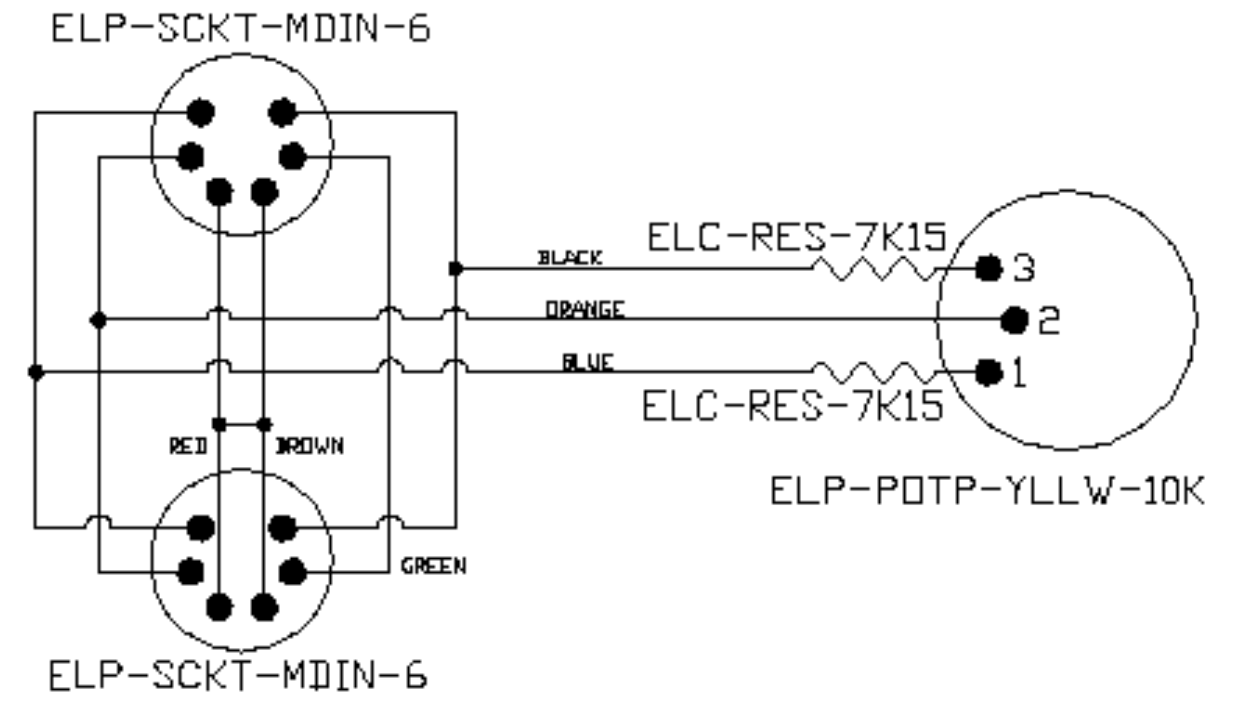
\includegraphics[width=0.4\columnwidth]{potentiometer_scheme}
	\caption{Potentiometer electrical scheme}
\end{figure*}
% trasformazione volt->rad fallita: non viene letta +-5V ma di meno
% tolto il modulo, per avere posizione incrementale su più giri
% interpolazione dei punti mancanti negli 8° di buco
% osservazione che pendenza della posizione è scorretta (causa tensione imprecisa)
% impossibilità di usare potenziometro come sensore di posizione/velocità durante il funzionamento, ma solo come posizione iniziale
% potenziomentro comunque impreciso di per sé

The total output range of the sensor should be ±5 V over the full 352° range.
The first passage to obtain the motor position is converting the voltage measured in radiants:
\[
	\theta_l = \bigl{(} V_{meas} - V_1 \bigr{)} \frac{352 \degree }{V_3 - V_1} \frac{\pi}{180 \degree }
\]

\subparagraph{Sensor calibration}
Actually, a variation of the voltage range must be considered: at the ends of the potentiometer sensor, voltage reading is not exactely $\pm 5V$, due to resistance variations from the nominal value. By observing the data collected, the usual maximum and minimum voltages are respectively~$V_3=4.67 \ V$ and~$V_1=-4.88 \ V$.

The sensor is able to detect the position along only one turn, then an incremental position that considers also the number of turns must be computed via software.
In particular, a Matlab script for post-processing elaboration of data has been written. This is able to recognize the end of a turn and the beginning of the next one; thanks to this, it remembers the number of revolutions and rearranges all the data according to that.

Moreover, the gap of~$8 \degree$ can be fitted by interpolating the two values around it. Notice that this procedure works only in case the motor speed is quite constant in time.

% figure script potentiometer
Unfortunately it is visible that the sensor data are very imprecise: the slope of the curve is not continuous. For this reason, real time measurements for motor position and speed are not reliable; we use only the initial position because it is useful for controlling absolute position and  during simulations.
\begin{figure*}
	\centering
	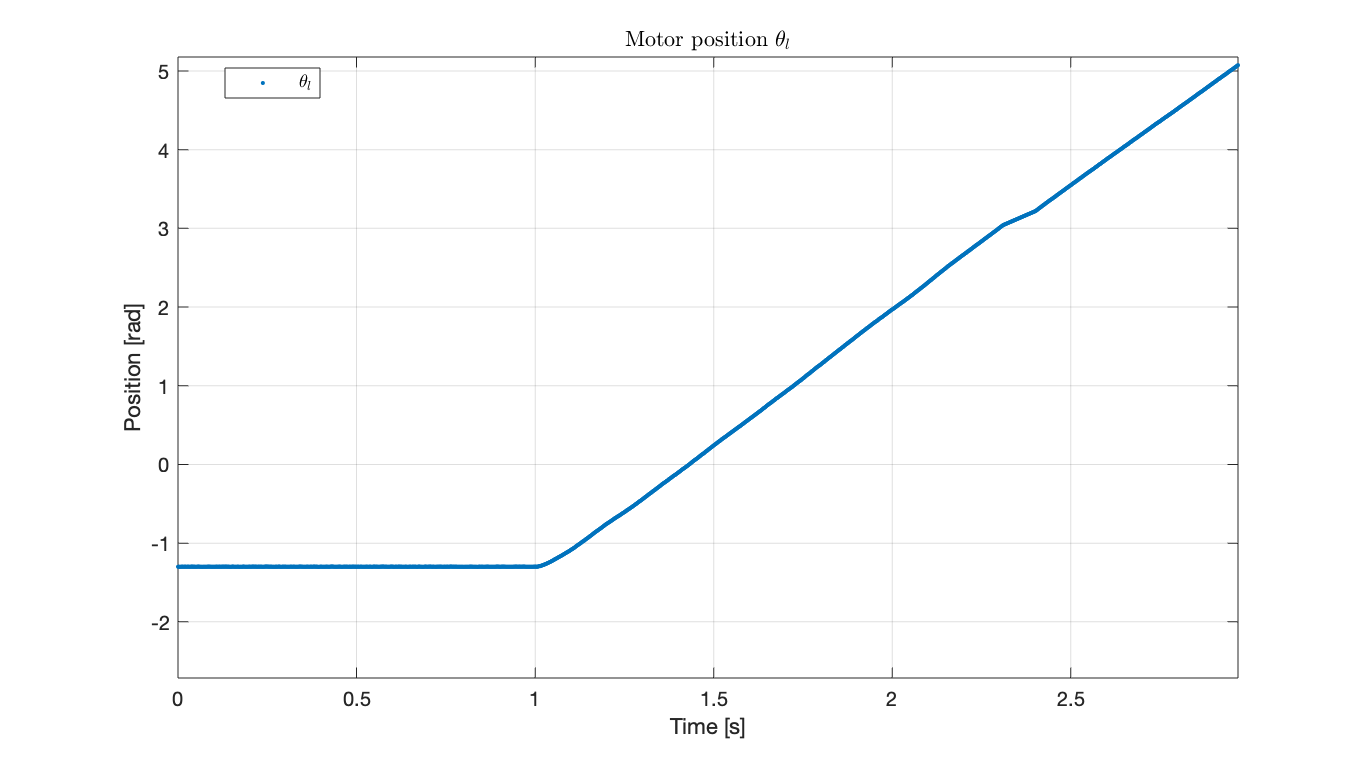
\includegraphics[width=\columnwidth]{pote_recover}
	\caption{Potentiometer data post-processing}
\end{figure*}

\paragraph{Encoder}

The encoder is a digital sensor that reads angular motions. It generates a pulse every small movement (both clockwise or counter-clockwise, detecting the direction of the motion) and, thanks to a counter, gives an incremental measurement with respect to the initial position. One revolution includes 4096 pulses, so the formula to obtain the position is the following:
\[
	\theta_x = \frac{2\pi}{4096} \ y \qquad x={1,2}
\]
The~$y$ signal is the processed one by the following Matlab function:
\begin{verbatim}
	function y = fcn(u)
	persistent oldu;
	persistent buffer;
	persistent oldy;
	if isempty(oldu)
	oldu=0;
	oldy = 0;
	buffer = 0;
	end
	
	% subtract the very first value of the experiment
	if u~=0 & oldu==0 
	oldu=u;
	end
	y=u-oldu;
	
	if ( y - oldy > 33000 )
	buffer = buffer-1;
	elseif ( y - oldy < - 33000 )
	buffer = buffer+1;
	end
	oldy = y;
	
	y = y + buffer*2^16;
\end{verbatim}
This code is able to impose the initial condition of the masses position to~$0$ (notice that the buffer is not reset after an experiment, hence an incorrect value at the motion starting of the following experiment would be given). Moreover, it must be considered that the buffer storage has dimention 16 bits, with values between $-32.768$ and $32.767$. Once a limit of the buffer is reached, an overflow occurs and the Matlab function is able to overcome this problem by returning a greater number. The result is the correct relative motion from the beginning of the experiment.

\subparagraph{Uncertainty and noise}

The digital encoder has a resolution determined by the number of pulses per revolution:
\[
	R = \frac{1}{4096}
\]
Thus, each measurement can be seen as a uniform distribution of probability between the two adjacent pulses; the distance of the true position from the measured one can be expressed as a Gaussian probability distribution function, whose variance defines the measurement uncertainty:
\begin{align*}
	U &= \frac{(2R)^2}{12} \\
	\Theta_{enc} &\sim \Gamma \bigl{(} 0,\frac{(2R)^2}{12} \bigr{)} = \Gamma \bigl{(} 0, 2e-8 \bigr{)}
\end{align*}

\subparagraph{Speed}

The speed of the two masses is obtainable by derivating the measument of the encoders. It is done thanks to the \textit{Discrete Derivative} Simulink block, that differentiates two consecutive values with respect to the sampling time:
\[
	\dot{\theta_l} = \frac{ \theta_{enc}(t) - \theta_{enc}(t-1)}{T_s}
\]
Due to the uncertainty of the encoder, the speed derivation is noisy, according to the following:
\begin{align*}
	U &= \frac{2(2R)^2}{12 {T_s}^2 } \\
	\dot{\Theta}_{enc}	&\sim \Gamma \bigl{(} 0,\frac{(2R)^2}{12 \ {T_s}^2} \bigr{)} + \Gamma \bigl{(} 0,\frac{(2R)^2}{12 \ {T_s}^2} \bigr{)} = \Gamma \bigl{(} 0, 0.001 \bigr{)}
\end{align*}
The uncertainty of the speed is extremely higher that the position one, so a low-pass filter is needed in order to reduce the measurement noise. The cutting frequency of the filter is determined by the higher resonance frequency of the system (shown later), such that the measurement is accurate up to that value:
\[
	F_{lp} = \frac{ \omega_f }{ s+\omega_f} \qquad \omega_f=25Hz=157.08 rad/s
\]
	\chapter{Model identification}
		\section{Mathematical description}

The physical model can be described by ordinary differential equations (ODEs), subdividing the system into single components: DC motor, gear, first spring, first mass, second spring, second mass. The parameters used are the nominal values defined in the manuals of components setup. This formulation of the problem can be useful in the following chapters, when the controller design will depend on the state-space realization or on the transfer functions.
\begin{figure*}[h]
	\centering
	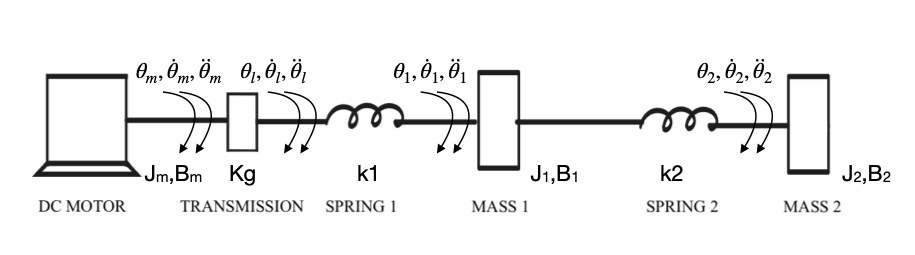
\includegraphics[width=0.8\columnwidth]{system_scheme}
	\caption{Scheme of the physical model}
\end{figure*}

% Equazioni componenti
\textit{Model of the motor and gear box}
\begin{subequations}
	\begin{align}
		V &= R_m i + L_m \frac{d}{dt}i + k_m \dot{\theta}_m \\
		\tau_m &= \eta_m k_t i \\
		\tau_{ml} &= \eta_g K_g \tau_m = \eta_m \eta_g K_g k_t i\\
		&= -J_m \ddot{\theta}_l - B_m \dot{\theta}_l - K_{s1} ( \theta_l - \theta_1 ) \qquad  \theta_l = \frac {1}{K_g} \theta_m \\
		\label{fig:model_equations}
	\end{align}
\end{subequations}

\textit{Model of the \acrshort{1-dof} system}
\begin{equation}
	J_1 \ddot{\theta}_1 + B_1 \dot{\theta}_1 = K_{s_1} ( \theta_l - \theta_1 )
\end{equation}

\textit{Model of the \acrshort{2-dof} system}
\begin{subequations}
	\begin{align}
		J_1 \ddot{\theta}_1 + B_1 \dot{\theta}_1 &= K_{s_1} ( \theta_l - \theta_1 ) - K_{s_2} ( \theta_1 - \theta_2 ) \\
		J_2 \ddot{\theta}_2 + B_2 \dot{\theta}_2 &= K_{s_2} ( \theta_1 - \theta_2 )
	\end{align}
\end{subequations}

% Forma di stato
\textit{State-space representation of the complete 1 d.o.f. system}
\begin{equation}
	\begin{bmatrix}
		\dot{i} \\
		\dot{\theta}_l \\
		\ddot{\theta}_l \\
		\dot{\theta}_1 \\
		\ddot{\theta}_1
	\end{bmatrix}
	=
	\begin{bmatrix}
		-\frac{R_m}{L_m} & 0 & -\frac{k_m K_g}{L_m} & 0 & 0 \\
		0 & 0 &1 & 0 & 0 \\
		\frac{\eta_m \eta_g k_t K_g}{J_m} & -\frac{K_{s_1}}{J_m} & -\frac{B_m}{J_m} & \frac{K_{s_1}}{J_m} & 0 \\
		0 & 0 & 0 & 0 & 1 \\
		0 & \frac{K_{s_1}}{J_1} & 0 & -\frac{K_{s_1}}{J_1} & -\frac{B_1}{J_1}
	\end{bmatrix}
	\begin{bmatrix}
		i \\
		\theta_l \\
		\dot{\theta}_l \\
		\theta_1 \\
		\dot{\theta}_1
	\end{bmatrix}
	+
	\begin{bmatrix}
		\frac{1}{L_m} \\
		0 \\
		0 \\
		0 \\
		0
	\end{bmatrix}
	V
\end{equation}

\textit{State-space representation of the complete 2 d.o.f. system}
\begin{equation}
	\begin{bmatrix}
		\dot{i} \\
		\dot{\theta}_l \\
		\ddot{\theta}_l \\
		\dot{\theta}_1 \\
		\ddot{\theta}_1 \\
		\dot{\theta}_2 \\
		\ddot{\theta}_2
	\end{bmatrix}
	=
	\begin{bmatrix}
		-\frac{R_m}{L_m} & 0 & -\frac{k_m K_g}{L_m} & 0 & 0 & 0 & 0 \\
		0 & 0 &1 & 0 & 0 & 0 & 0 \\
		\frac{\eta_m \eta_g k_t K_g}{J_m} & -\frac{K_{s_1}}{J_m} & -\frac{B_m}{J_m} & \frac{K_{s_1}}{J_m} & 0 & 0 & 0 \\
		0 & 0 & 0 & 0 & 1 & 0 & 0 \\
		0 & \frac{K_{s_1}}{J_1} & 0 & -\frac{K_{s_1}+K_{s_2}}{J_1} & -\frac{B_1}{J_1} & \frac{K_{s_2}}{J_1} & 0 \\
		0 & 0 & 0 & 0 & 0 & 0 & 1 \\
		0 & 0 & 0 & \frac{K_{s_2}}{J_2} & 0 & -\frac{K_{s_2}}{J_2} & -\frac{B_2}{J_2}
	\end{bmatrix}
	\begin{bmatrix}
		i \\
		\theta_l \\
		\dot{\theta}_l \\
		\theta_1 \\
		\dot{\theta}_1 \\
		\theta_2 \\
		\dot{\theta}_2
	\end{bmatrix}
	+
	\begin{bmatrix}
		\frac{1}{L_m} \\
		0 \\
		0 \\
		0 \\
		0 \\
		0 \\
		0
	\end{bmatrix}
	V
\end{equation}

From this mathematical formulation, it is easy to check (thanks to MATLAB functions  \textit{ctrb} e \textit{obsv}) the controllability by means of the voltage applied to the motor and the system observability.
The system having just one rotating mass is controllable only in two state variables over five: surely, one of those is the current (directly affected by the input), the other is one among the remaining. On the other hand, the observability matrix~$M_O$ is full rank; however, it must be considered that the current~$i$ dynamics is extremely rapid (the time constant is defined as~$\tau_i = \frac{L_m}{R_m} = 7.56\ 10^{-5} \ s$), then the sampling time~($T_s = 2 ms$) prevents its observation even with a current sensor installed on the motor.
Similarly to this case, it can be expected that also the 2-d.o.f. system is not fully controllable. \\

Since the current dynamics cannot be verified by experimental data, we have decided to ignore it~(the rest of the model is not significantly affected by that, since its transient is definitely negligible): in the following model, the current statically depends on the input voltage and the electromotive force (back-emf).\\
% Forma di stato ridotta
\textit{State-space representation of the reduced 1-d.o.f. system}
\begin{equation}
	\begin{bmatrix}
		\dot{\theta}_l \\
		\ddot{\theta}_l \\
		\dot{\theta}_1 \\
		\ddot{\theta}_1
	\end{bmatrix}
	=
	\begin{bmatrix}
		0 &1 & 0 & 0 \\
		-\frac{K_{s_1}}{J_m} & -\frac{B_m}{J_m}-\frac{\eta_m \eta_g k_t k_m {K_g}^2}{R_m J_m}  & \frac{K_{s_1}}{J_m} & 0 \\
		0 & 0 & 0 & 1 \\
		\frac{K_{s_1}}{J_1} & 0 & -\frac{K_{s_1}}{J_1} & -\frac{B_1}{J_1}
	\end{bmatrix}
	\begin{bmatrix}
		\theta_l \\
		\dot{\theta}_l \\
		\theta_1 \\
		\dot{\theta}_1
	\end{bmatrix}
	+
	\begin{bmatrix}
		0 \\
		\frac{\eta_m \eta_g k_t K_g}{R_m J_m} \\
		0 \\
		0
	\end{bmatrix}
	V
\end{equation}

\textit{State-space representation of the reduced 2-d.o.f. system}
\begin{equation}
	\begin{bmatrix}
		\dot{\theta}_l \\
		\ddot{\theta}_l \\
		\dot{\theta}_1 \\
		\ddot{\theta}_1 \\
		\dot{\theta}_2 \\
		\ddot{\theta}_2
	\end{bmatrix}
	=
	\begin{bmatrix}
		0 &1 & 0 & 0 & 0 & 0 \\
		-\frac{K_{s_1}}{J_m} & -\frac{B_m}{J_m}-\frac{\eta_m \eta_g k_t k_m {K_g}^2}{R_m J_m}  & \frac{K_{s_1}}{J_m} & 0 & 0 & 0 \\
		0 & 0 & 0 & 1 & 0 & 0 \\
		\frac{K_{s_1}}{J_1} & 0 & -\frac{K_{s_1}+K_{s_2}}{J_1} & -\frac{B_1}{J_1} & \frac{K_{s_2}}{J_1} & 0 \\
		0 & 0 & 0 & 0 & 0 & 1 \\
		0 & 0 & \frac{K_{s_2}}{J_2} & 0 & -\frac{K_{s_2}}{J_2} & -\frac{B_2}{J_2}
	\end{bmatrix}
	\begin{bmatrix}
		\theta_l \\
		\dot{\theta}_1 \\
		\theta_1 \\
		\dot{\theta}_1 \\
		\theta_2 \\
		\dot{\theta}_2
	\end{bmatrix}
	+
	\begin{bmatrix}
		0 \\
		\frac{\eta_m \eta_g k_t K_g}{R_m J_m} \\
		0 \\
		0 \\
		0 \\
		0
	\end{bmatrix}
	V
\end{equation}
This time, checking again the controllability and observability of the reduced order system, matrices~$M_R$ e $M_O$ are full rank. \\

In order to validate this model, some experiments on the real system have been performed. Firstly, only one mass, then, two masses in cascade were linked to the shaft. By imposing to the motor a certain voltage, the open-loop response has been compared to the Simulink simulation (based on the model previously illustrated).

\paragraph{Experiments input}
The experiments, aimed at identifying and validating the model, have been performed by imposing a voltage to the motor. They can be classified in two types: steps (multiple in time and of different size) and variable frequency sine waves. The range of applied voltages~($\pm 10\ V$) is constrained by the motor physical limitations.

At first, the static gain of the transfer function between the control input of the motor and the first mass speed~($G_{V,\dot{\theta}_1}$) has been checked. To do so, a constant voltage has been imposed; once the transient of first mass settlement is over, it is clear that the mathematical model underestimates the steady-state speed.
The first approach has been that of changing the model parameters whose effect on the static gain is more significant: the rotor resistance~($R_m$), the motor efficiency~($\eta_m$), the mechanical efficiency of the gear~($\eta_g$), the current-torque constant~($k_t$) and the mass speed-voltage constant (~$k_m$, responsible of the back-emf).

Thanks to the experiments, it has been noticed that the real system behavior is not exactely linear with respect to the imposed voltage. Some physical interpretations have been proposed: the mechanical efficiency of the motor~($\eta_g$) is probably underestimated at low speeds; then, the~$k_m$ constant (that generates the back-emf), is very difficult to be estimated, since its effect on the motor power is quite significant at high speed, but almost negligible at low speed.

% parametri modificati ---> G_opt

The variable frequency sine wave experiments suggest another significant difference between the physical model and the nominal one. Here, it is visible that resonance frequency of the nominal model is greater that the real one; anyway, the amplitude of the oscillations at those frequencies is comparable. \\
This fact affects also the step response transient: the initial overshoot and later oscillations depend on complex conjugate poles, linked to the physical parameters of springs and masses (spring stiffness~$K_s$, mass inertia~$J$, mass friction coefficient~$B$). \\

A tuning of the static gain does not allow an improvement of the mathematical model in the transient behavior. However, manually changing all the other parameters would be particularly difficult, since it is a trial-and-error approach based on no precise rational reasoning (it must be considered also, indeed, that nominal parameters shown in the reference manual are obtained experimentally).
A solution to this problem is to untie our approach from the purely mathematical model (i.e. white-box) and use experimental data.

\section{Black-box identification}

\textit{Black-box identification with a parametric method of TF in time-domain} \\

\par A black-box approach totally loses a connection to the mathematical model and its physical dimensions; on the contrary, it is exclusively based on data collected by experiments in laboratory.
For this reason, it is reasonable to estimate only the transfer function of our interest (according to the design of the controller of speed, designed later):~$G_{V,\dot{\theta}_1}$ or~$G_{V,\dot{\theta}_2}$, meaning the transfer functions from the voltage (input) and the masses speed. \\

Masses speeds (generated by the derivation of encoder data) are collected in a set of experiments by using the Matlab functions~\textit{iddata()} e~\textit{merge()}. So, the obtained data are the input of the~\textit{tfest()} function: the obtained output is the identified black-box model. \\

Keeping in mind that the transfer function only sees observable and controllable poles, a first method to impose the number of poles in the identification function is looking at the computer results: if the obtained transfer function does not change by adding more poles, then the order of the system has been obtained.
By this procedure, it has been found a~$3^{rd}$ order transfer function, with 2 positive-real part zeros: in this way, the phase loss at high frequency of the nominal and empirical models coincide. On the other hand, the gain at that frequency is much less inclined.

\begin{figure*}[h]
	\centering
	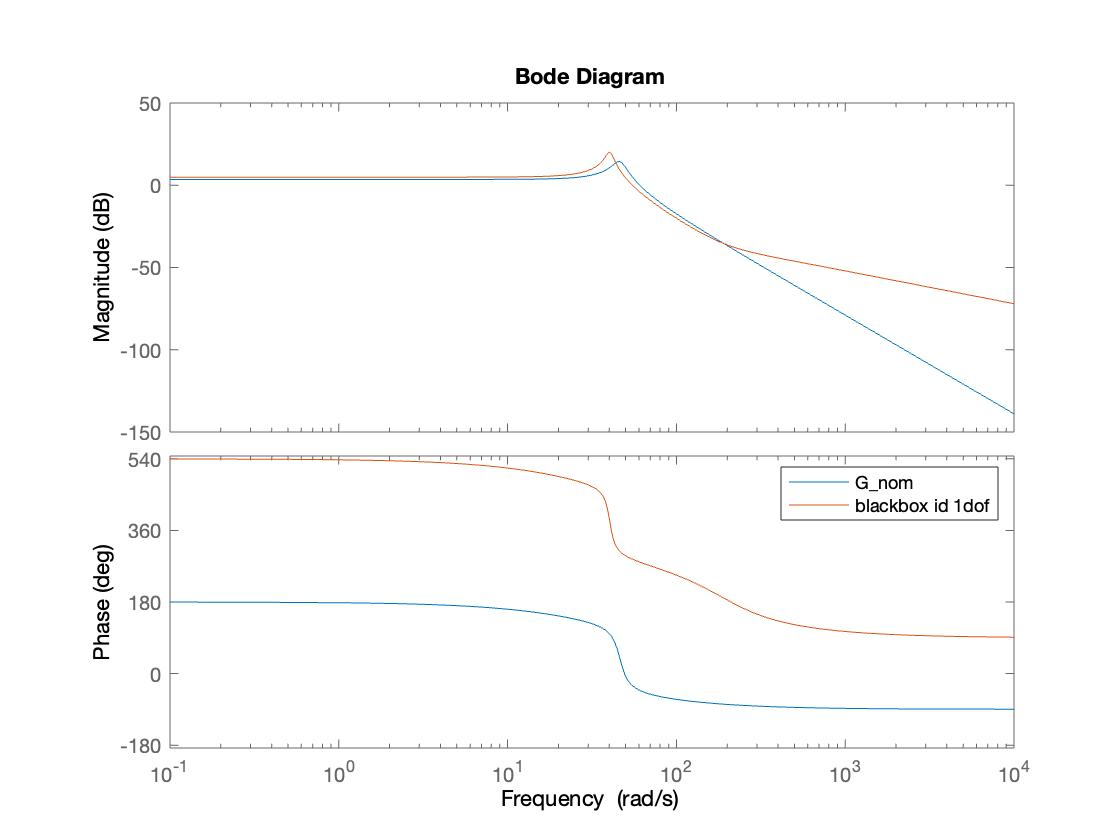
\includegraphics[width=\columnwidth]{black_1dof_withZeros}
	\caption{1-dof system. Transfer functions comparison, with zeros in blackbox}
\end{figure*}
\begin{figure*}[h]
	\centering
	\begin{subfigure}{\columnwidth}
%		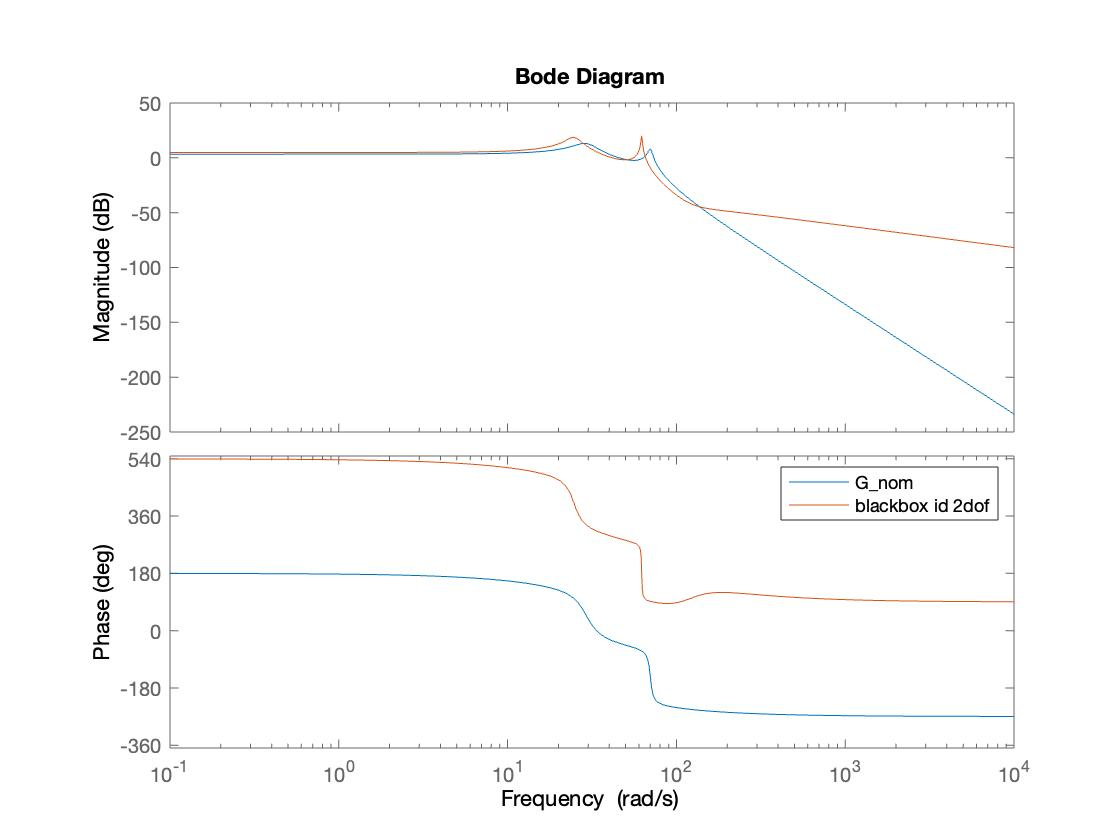
\includegraphics[width=\columnwidth]{black_2dof_withZeros}
	\end{subfigure}
	\begin{subfigure}{\columnwidth}
		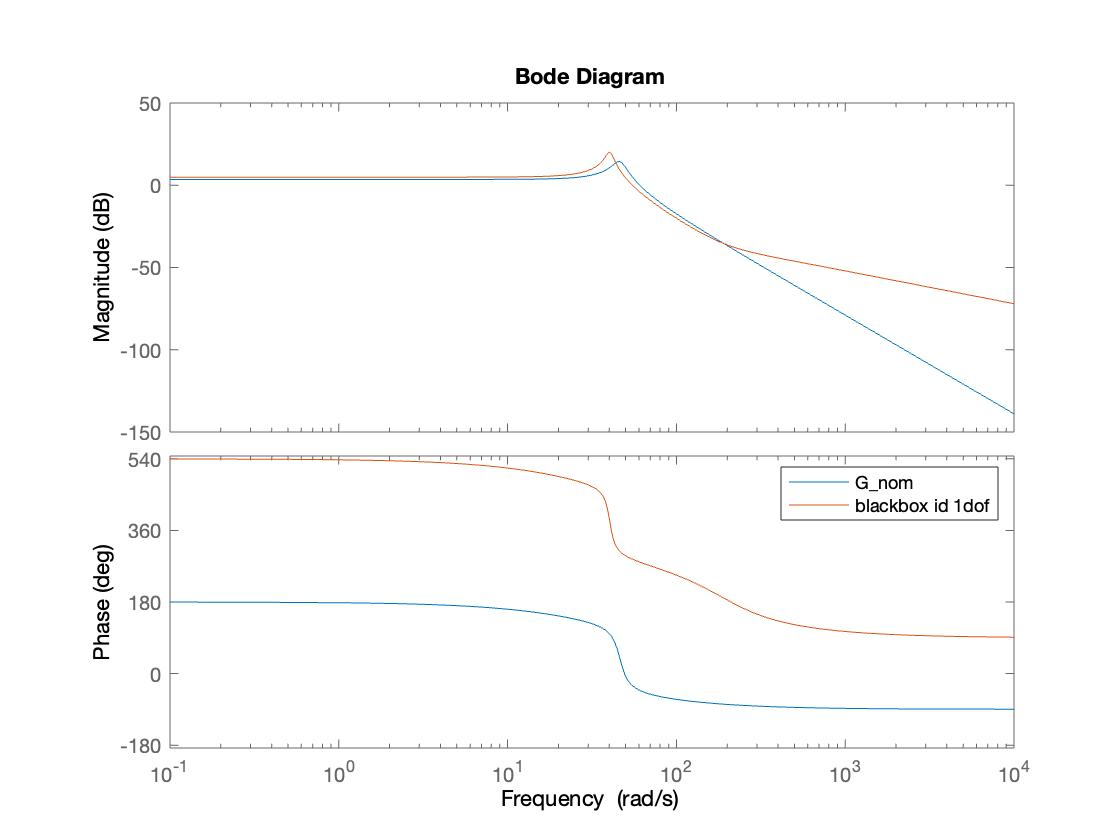
\includegraphics[width=\columnwidth]{black_1dof_withZeros}
	\end{subfigure}
	\caption{2-dof system. Transfer functions comparison, with zeros in blackbox}
\end{figure*}

To overcome this problem, it has been decided to impose the number of both poles and zeros, to be equal to the transfer function structure computed from the white-box model. Therefore, the 1 dof system has 3 poles and 0 zeros, while the 2 dof system has 5 poles and 0 zeros.
In addition to the physical model poles, it must be considered the low-pass filter for the speed measurement noise. \\
In this way, both module and phase Bode diagrams are very similar to the mathematical ones at every frequency.

\begin{figure*}[h]
	\centering
	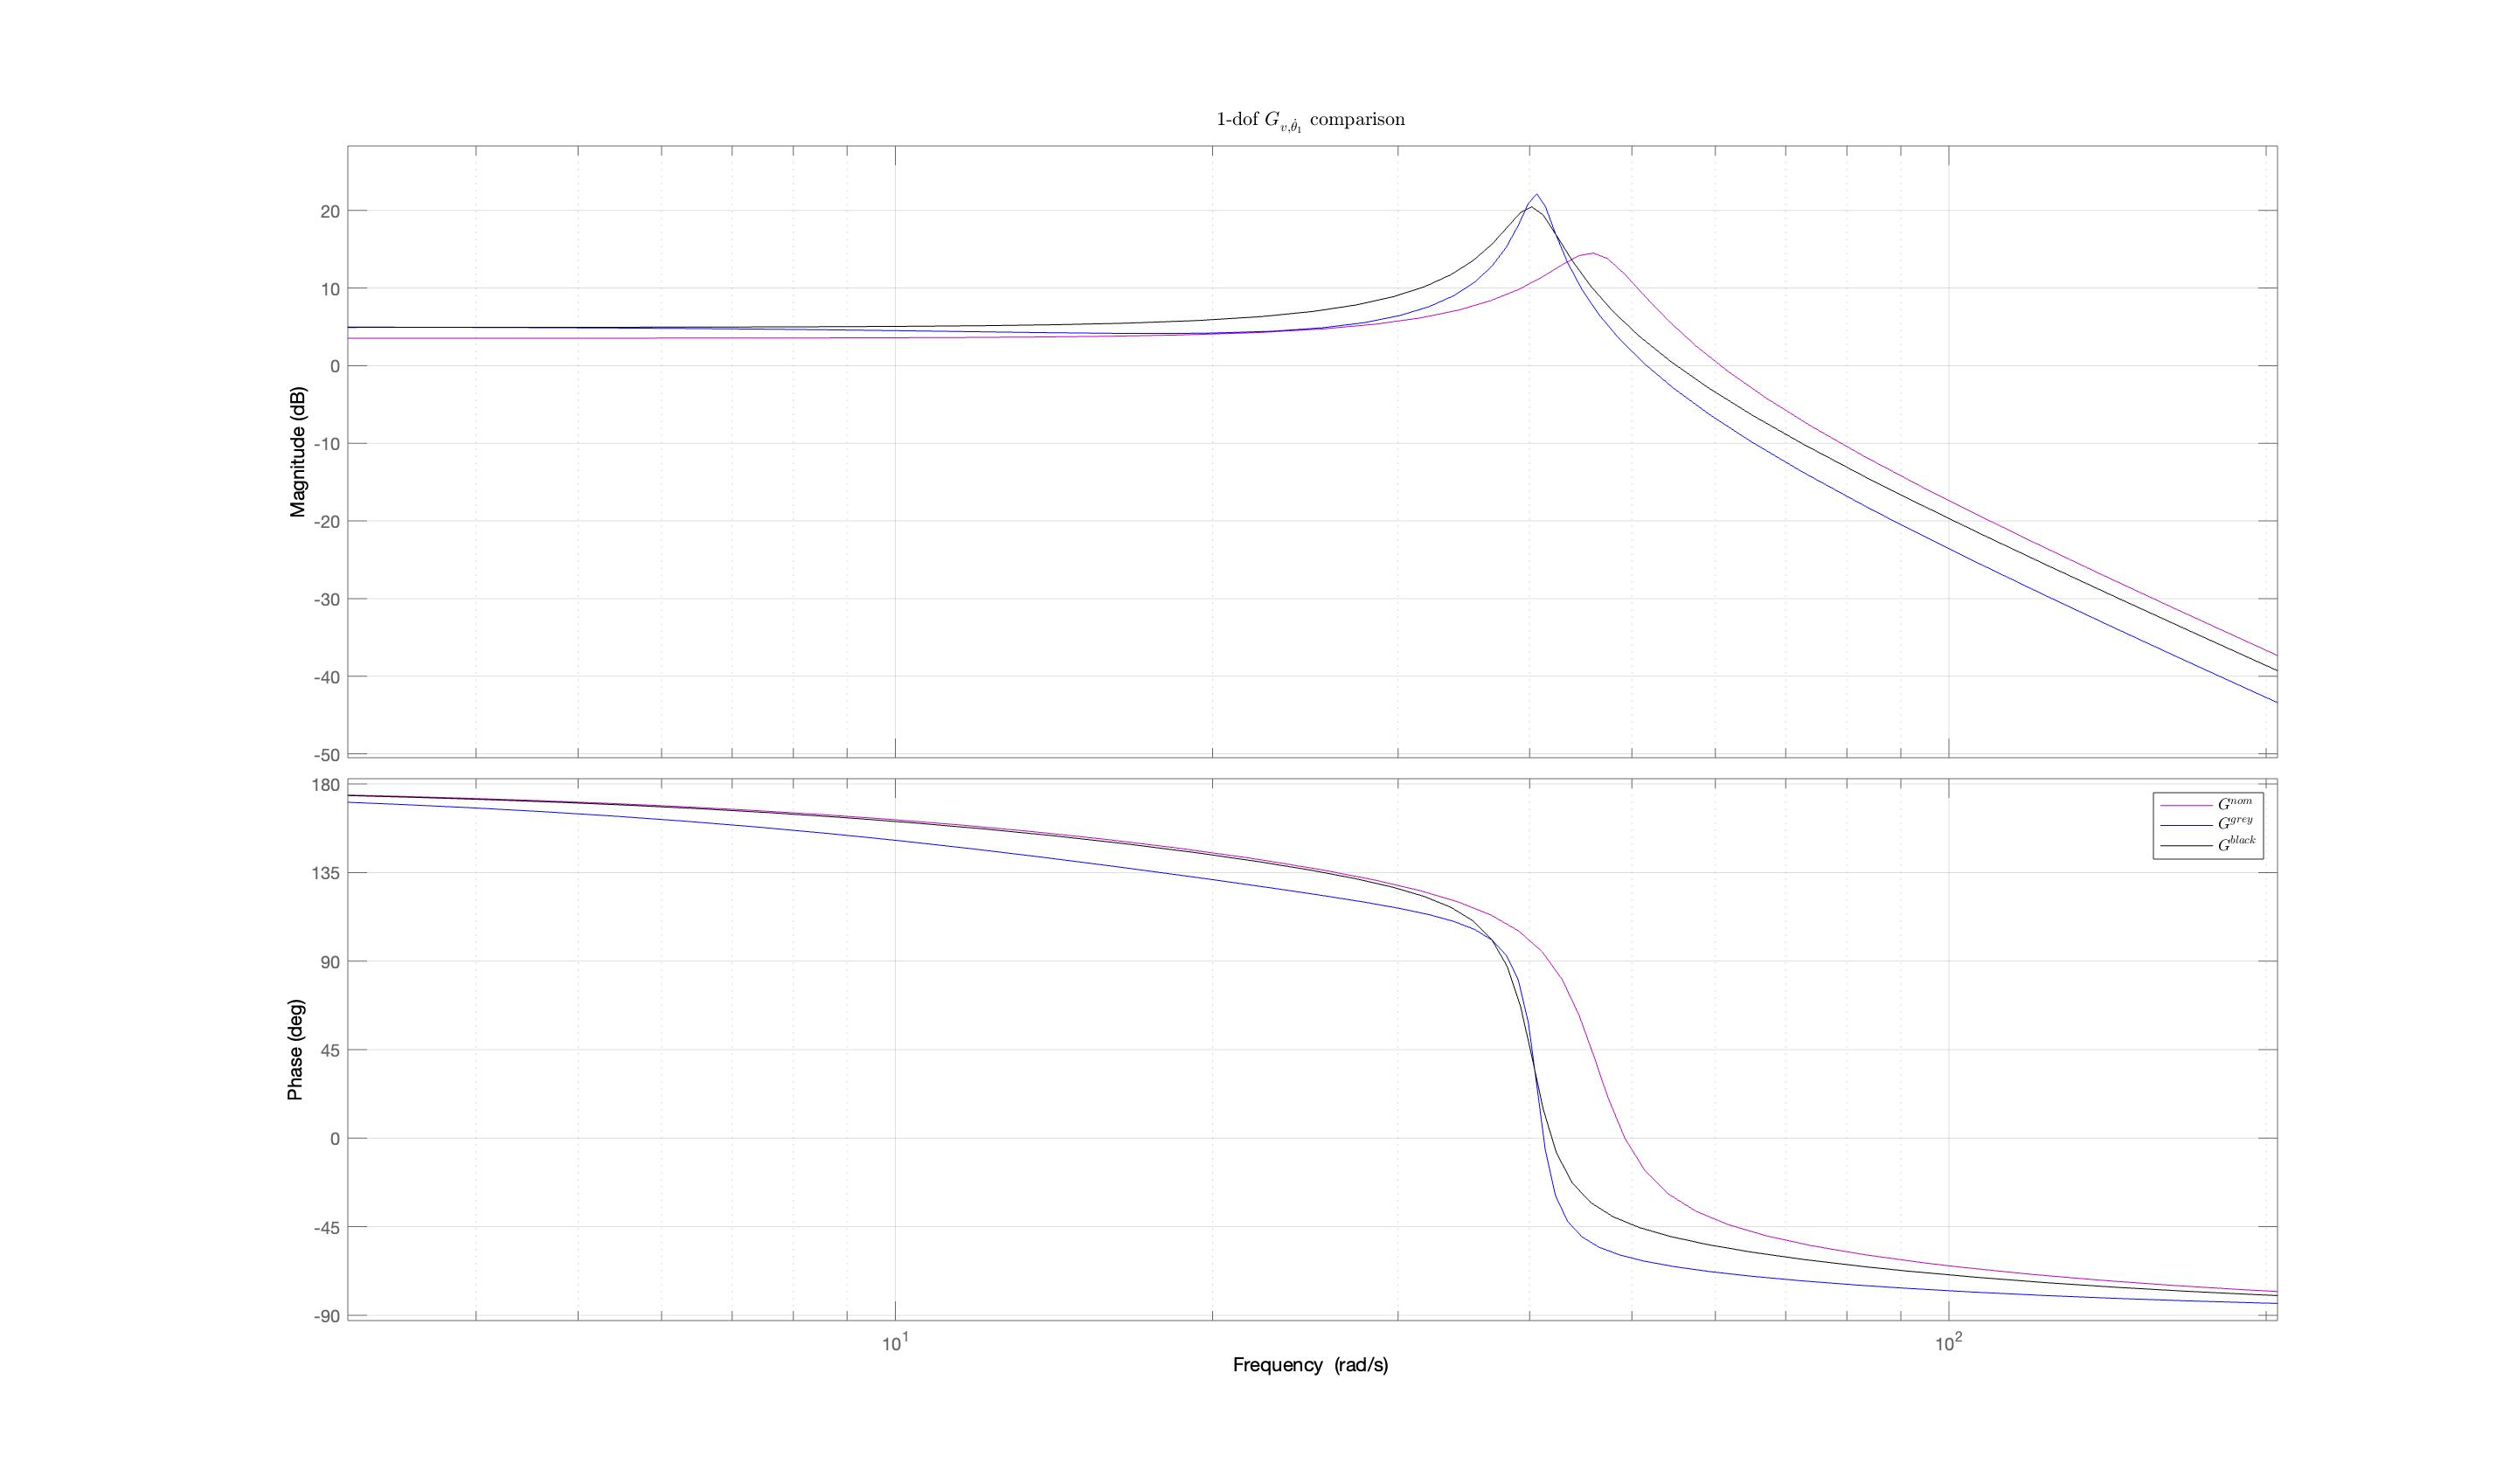
\includegraphics[width=\columnwidth]{1dof_g_v_w1}
	\caption{1-dof system. Transfer functions comparison, no zeros in blackbox}
\end{figure*}

\begin{figure*}[h]
	\centering
	\begin{subfigure}{0.45\columnwidth}
		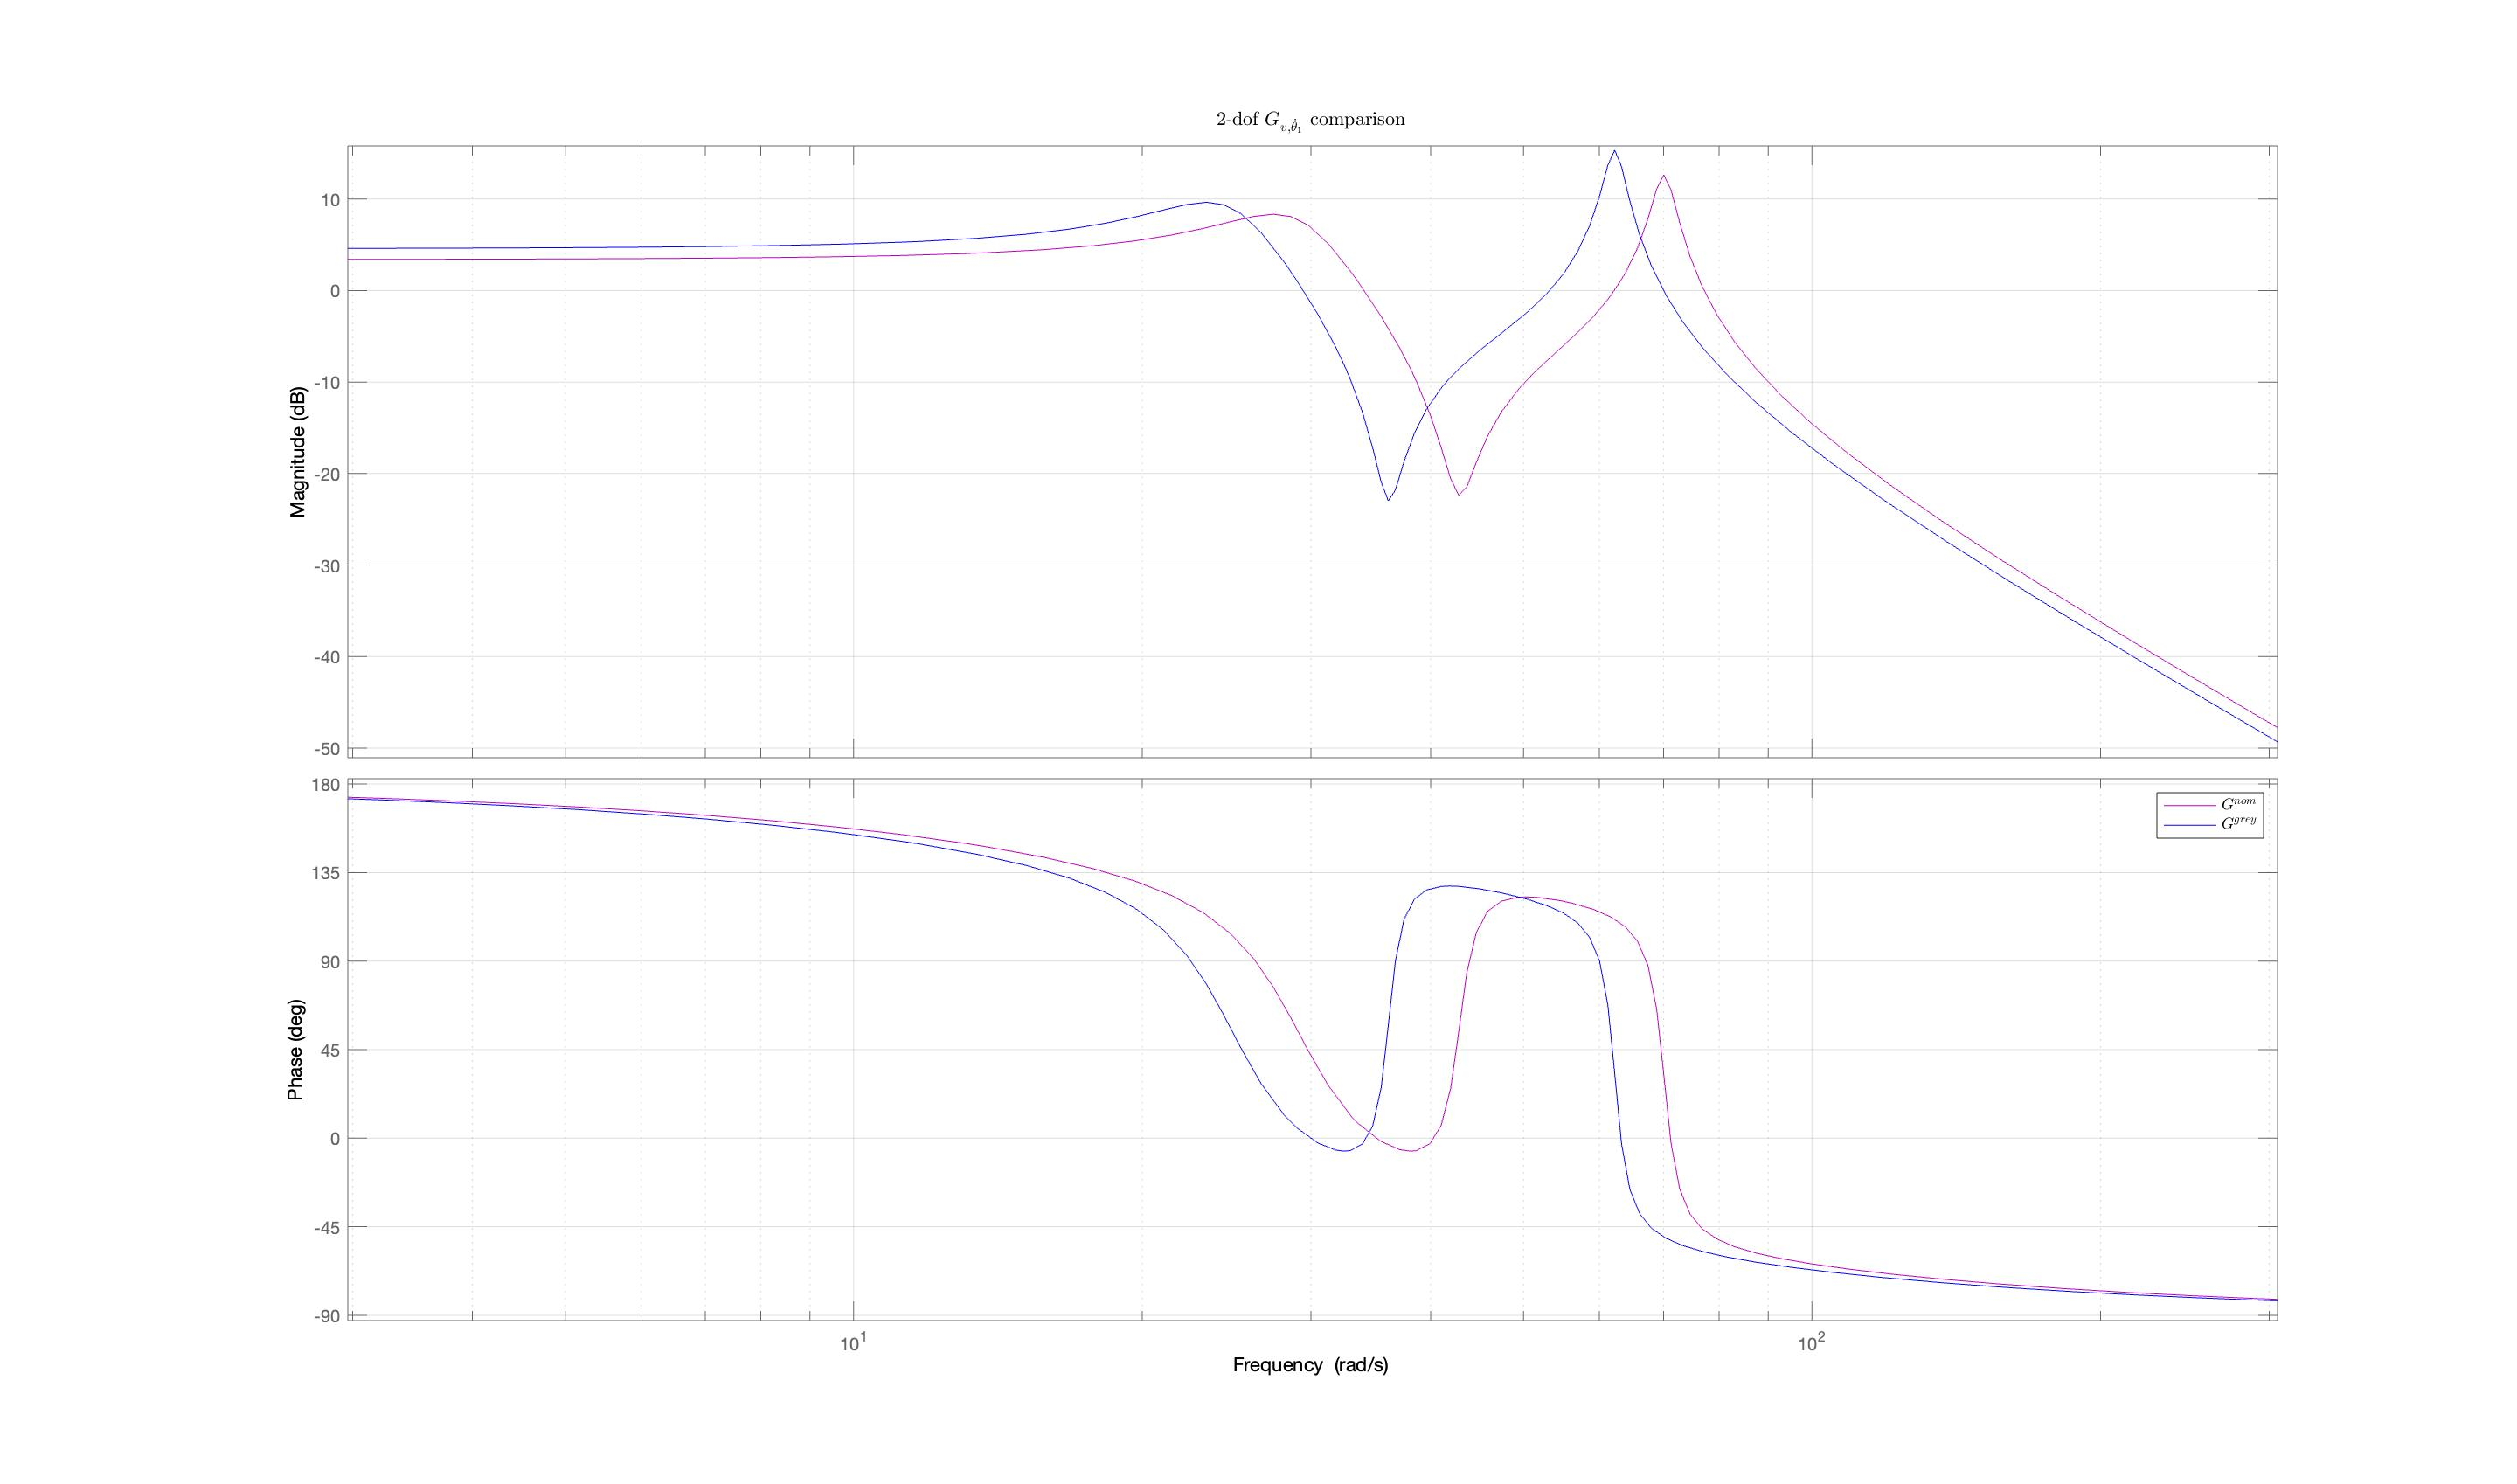
\includegraphics[width=\textwidth]{2dof_g_v_w1}
	\end{subfigure}
	\begin{subfigure}{0.45\columnwidth}
		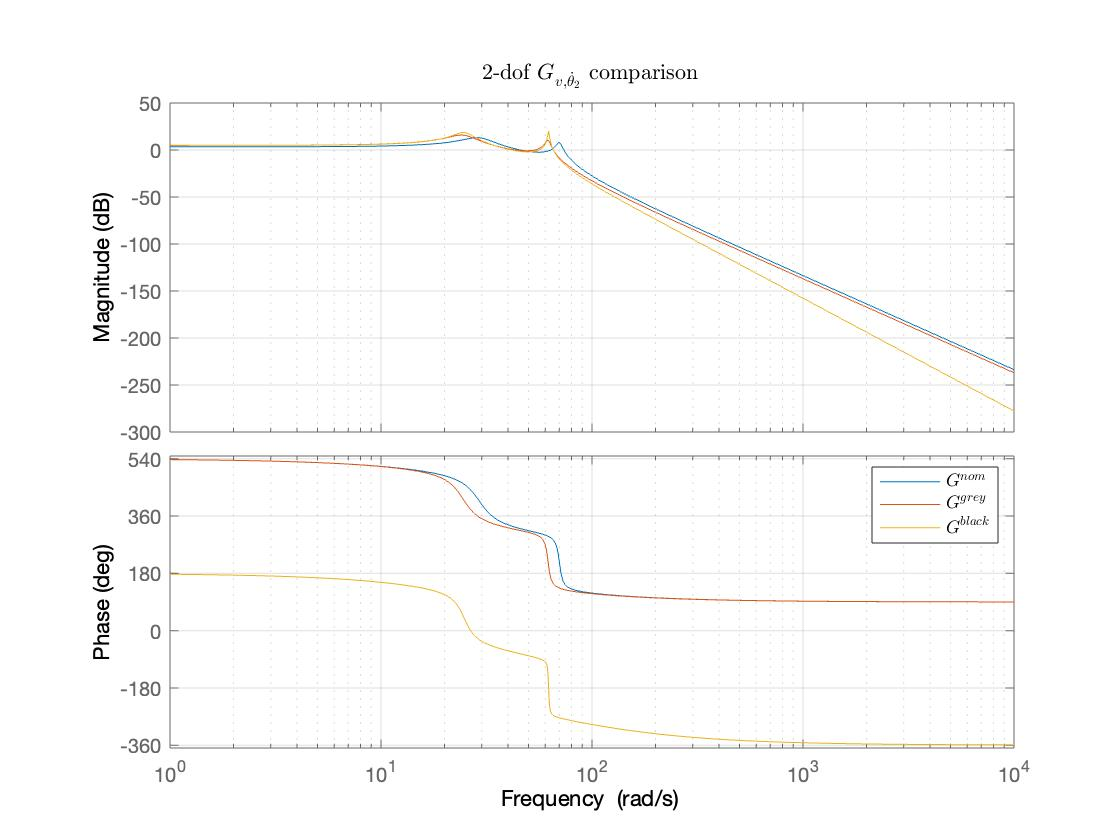
\includegraphics[width=\textwidth]{2dof_g_v_w2}
	\end{subfigure}
	\caption{2-dof system. Transfer functions comparison, no zeros in blackbox}
\end{figure*}

Following this approach, it has been observed that the resonance frequency of the identified model is lower that the nominal one, as the damping too.
Those differences can be immediately seen is the laboratory experiments: in particular, the ones with variable frequency sine wave. \\
It is important to remember that the speed measurement is noisy (the filter acts at very high frequency), because of the derivation from encoder data. Hence, obtaining the position, by integrating the speed estimated by this model, would generate a drift that increases in time.

Instead, trying to directly estimate~$G_{V,\theta_1}$ is not possible, since the black-box algorithm cannot place the integrator.

\section{Gray-box identification} \label{sec:gray_b_id}

\textit{Gray-box identification with a parametric error method of state-space time-domain} \\
\par The advantage of using a gray-box approach is that it maintains the mathematical model structure and tunes parameters based on experimental data. The starting model is defined on the nominal parameters (as illustrated in Paragraph "Mathematical description"), whose uncertainties are a-prior specified: in this way, the identification can change parameters in a well defined and constrained range, preserving a physical meaning. Specifically, masses parameters (inertia~$J$, friction~$B$) uncertainty is fixed manually~(the datasheet gives experimentally determined values); all the other parameters have an uncertainty range specified according to the reference manuals.
% table: nominal and identified parameters, uncertainty of param
% ragionare se controproducente !!!!!

Operatively, data experiments have been collected and the estimation of the model has been performed by means of the function~\textit{greyest()}. The used measurements include the position of both motor and masses: this allows to have a larger and differentiated set of data.

Identification results are very satisfactory: the precision of the model with respect to the motor position data are between~$70 / 95\%$, while the masses positions precision is about~$75 / 99\%$. The lower values of precision are obtained with low speed experiments.

The identified model has a resonance frequency located in between the nominal and black-box ones, as expected. Moreover, data collected in laboratory are very close to the simulation performed by using this identified model, thus, all the controllers are based on this identification. A confirm of the goodness of the identified model is the open-loop experiment at first mass anti-resonance frequency: in \cref{fig:antiresonance}, it is clear that, while the second mass has big oscillations, the first one is almost motionless. For the first mass, the magnitude should be about~$-20 dB$, indeed the oscillation amplitude is about 10 times smaller than applied voltage, while for the second at the same frequency it is around~$0 dB$, so oscillations amplitude is very close to applied voltage.
\begin{figure}
	\centering
	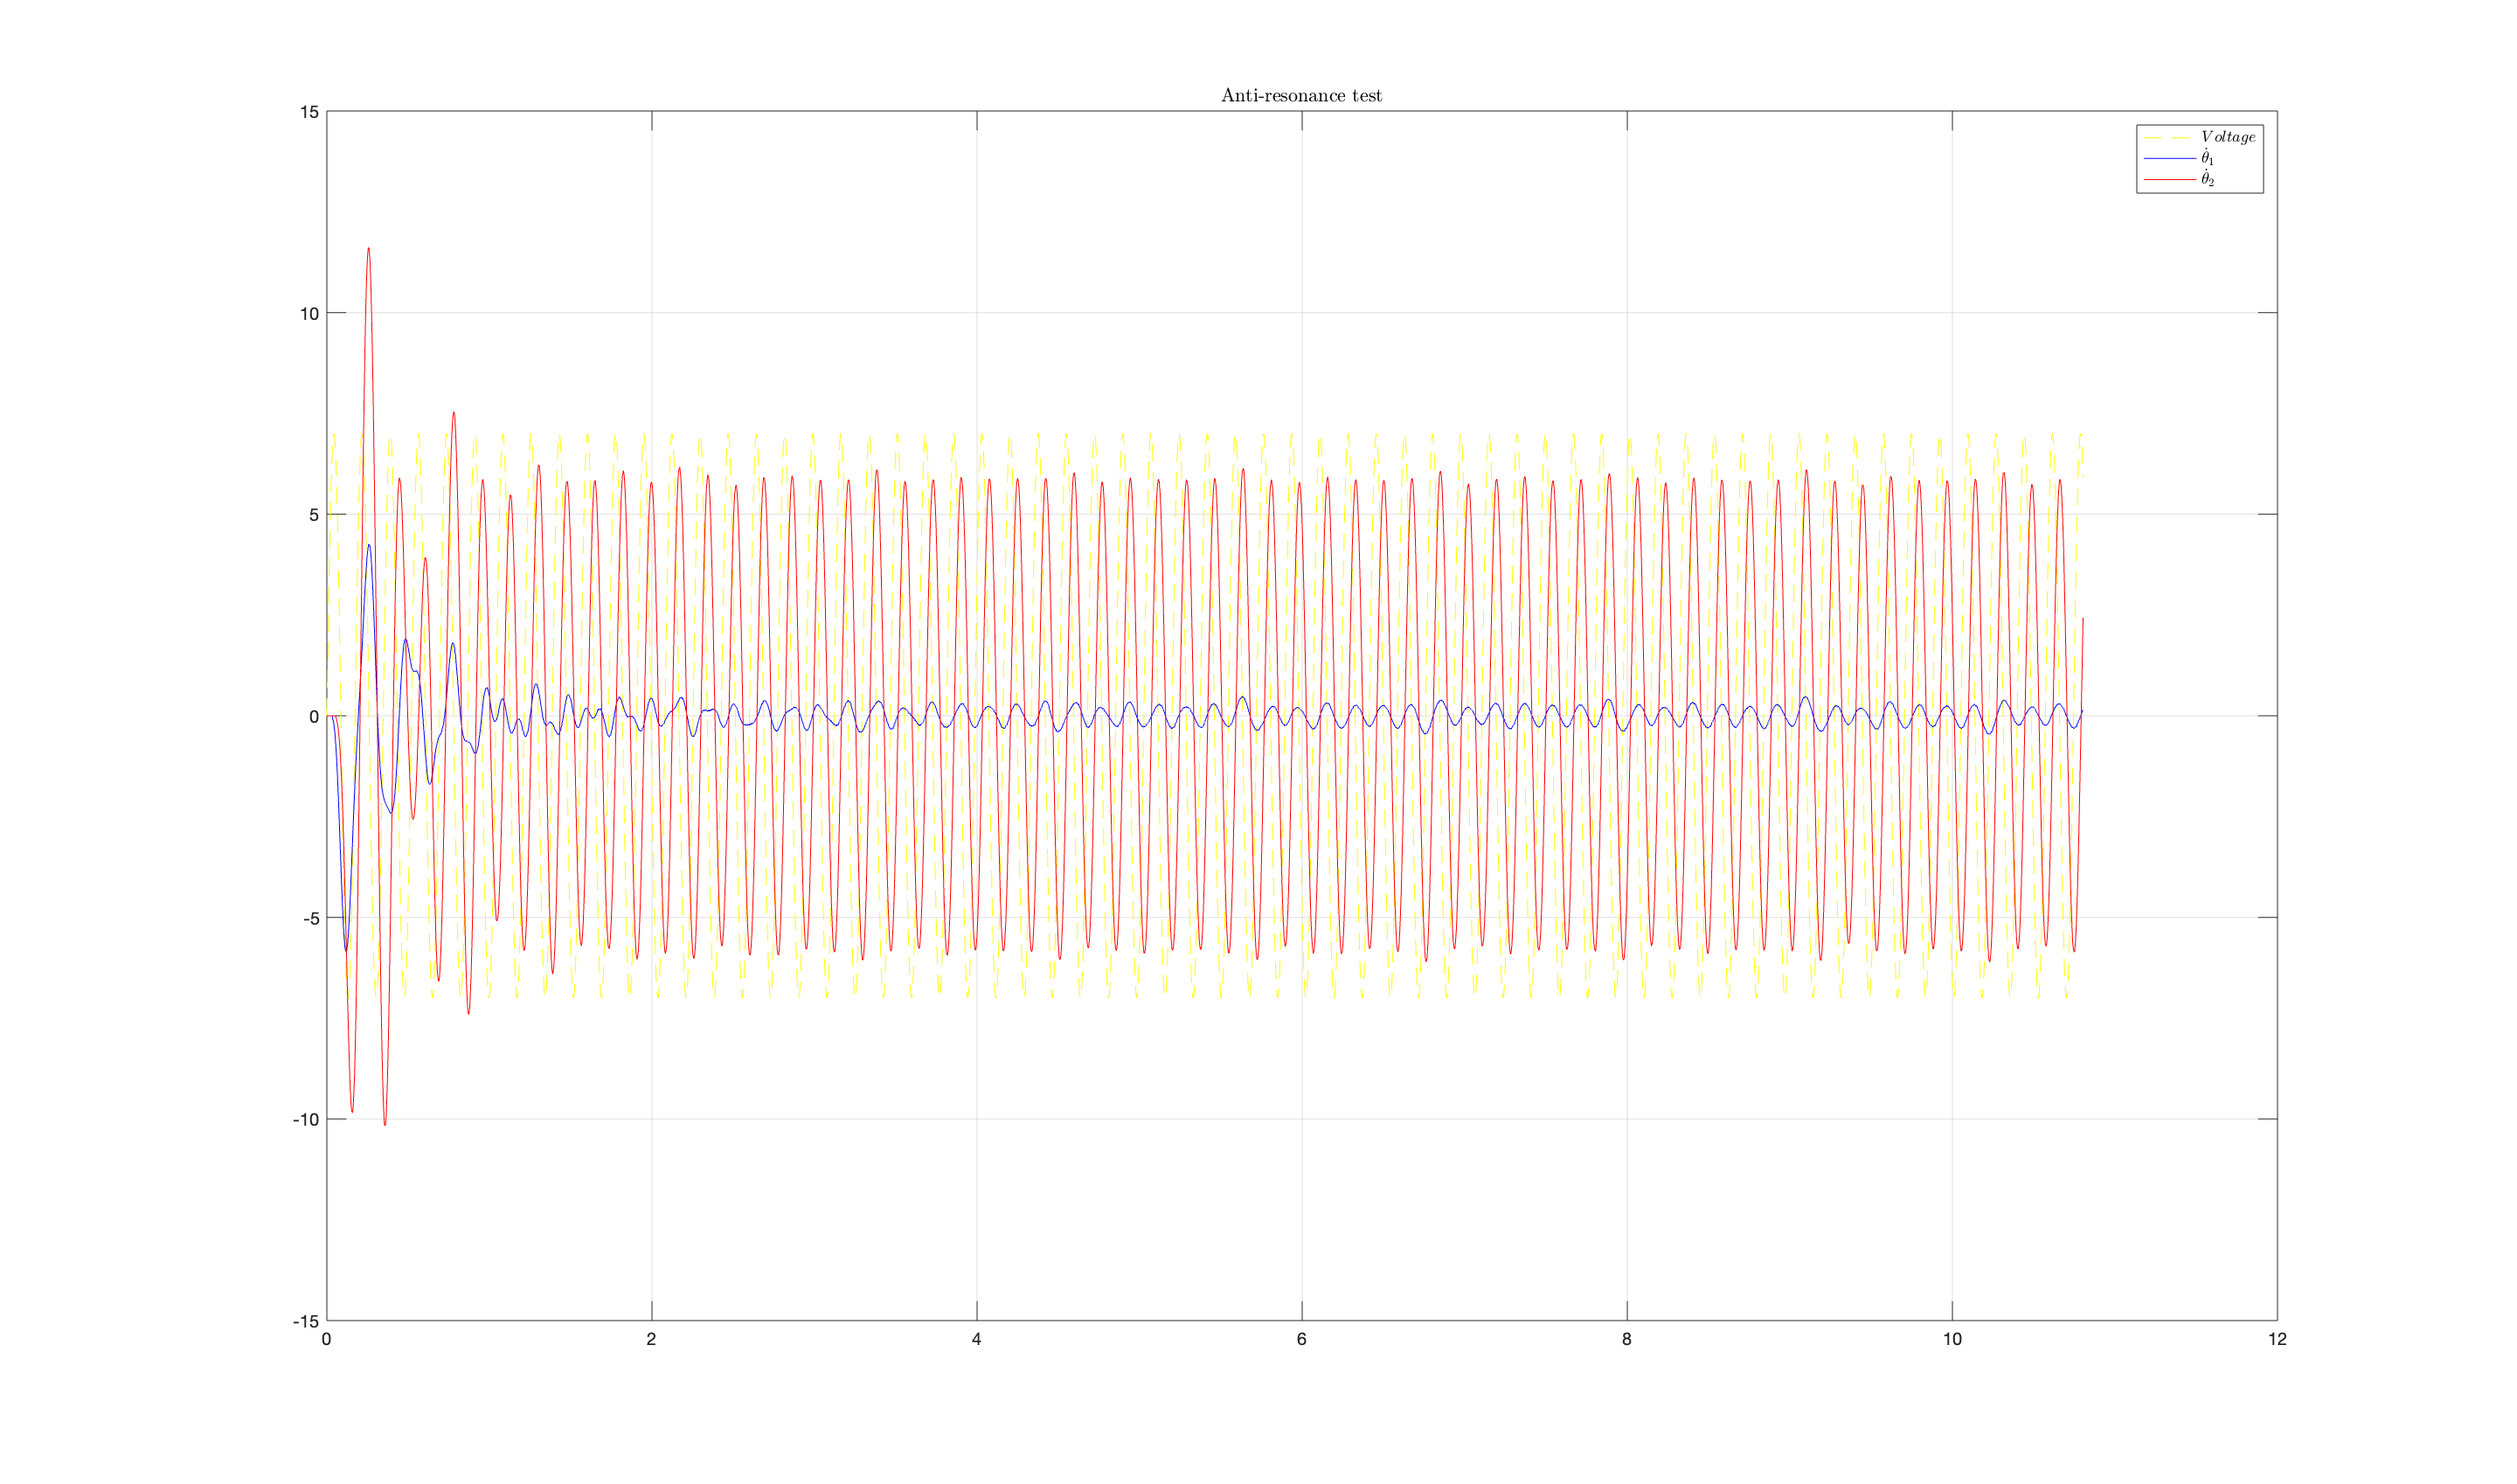
\includegraphics[width=0.6\columnwidth]{antiresonance_test}
	\caption{Sine-wave voltage: anti-resonance frequency}
	\label{fig:antiresonance}
\end{figure}

	\chapter{Controllers based on transfer functions}
		\label{sec:FD_control}
\section{\onedof\ system}
From now on, the controllers synthesis and simulations are based on the \textit{gray-box} model; here is reported the transfer function from the applied voltage to the first mass speed: \\
\[	
G_{v, \dot \theta_1}(s)=
\frac{-5.618 \cdot 10^{4}}{{s^3 + 21.45 s^{2}}+1699 s+3.149 \cdot 10^{4}}
\]

\begin{figure*}[h]
	\centering
	\begin{subfigure}{0.55\columnwidth}
		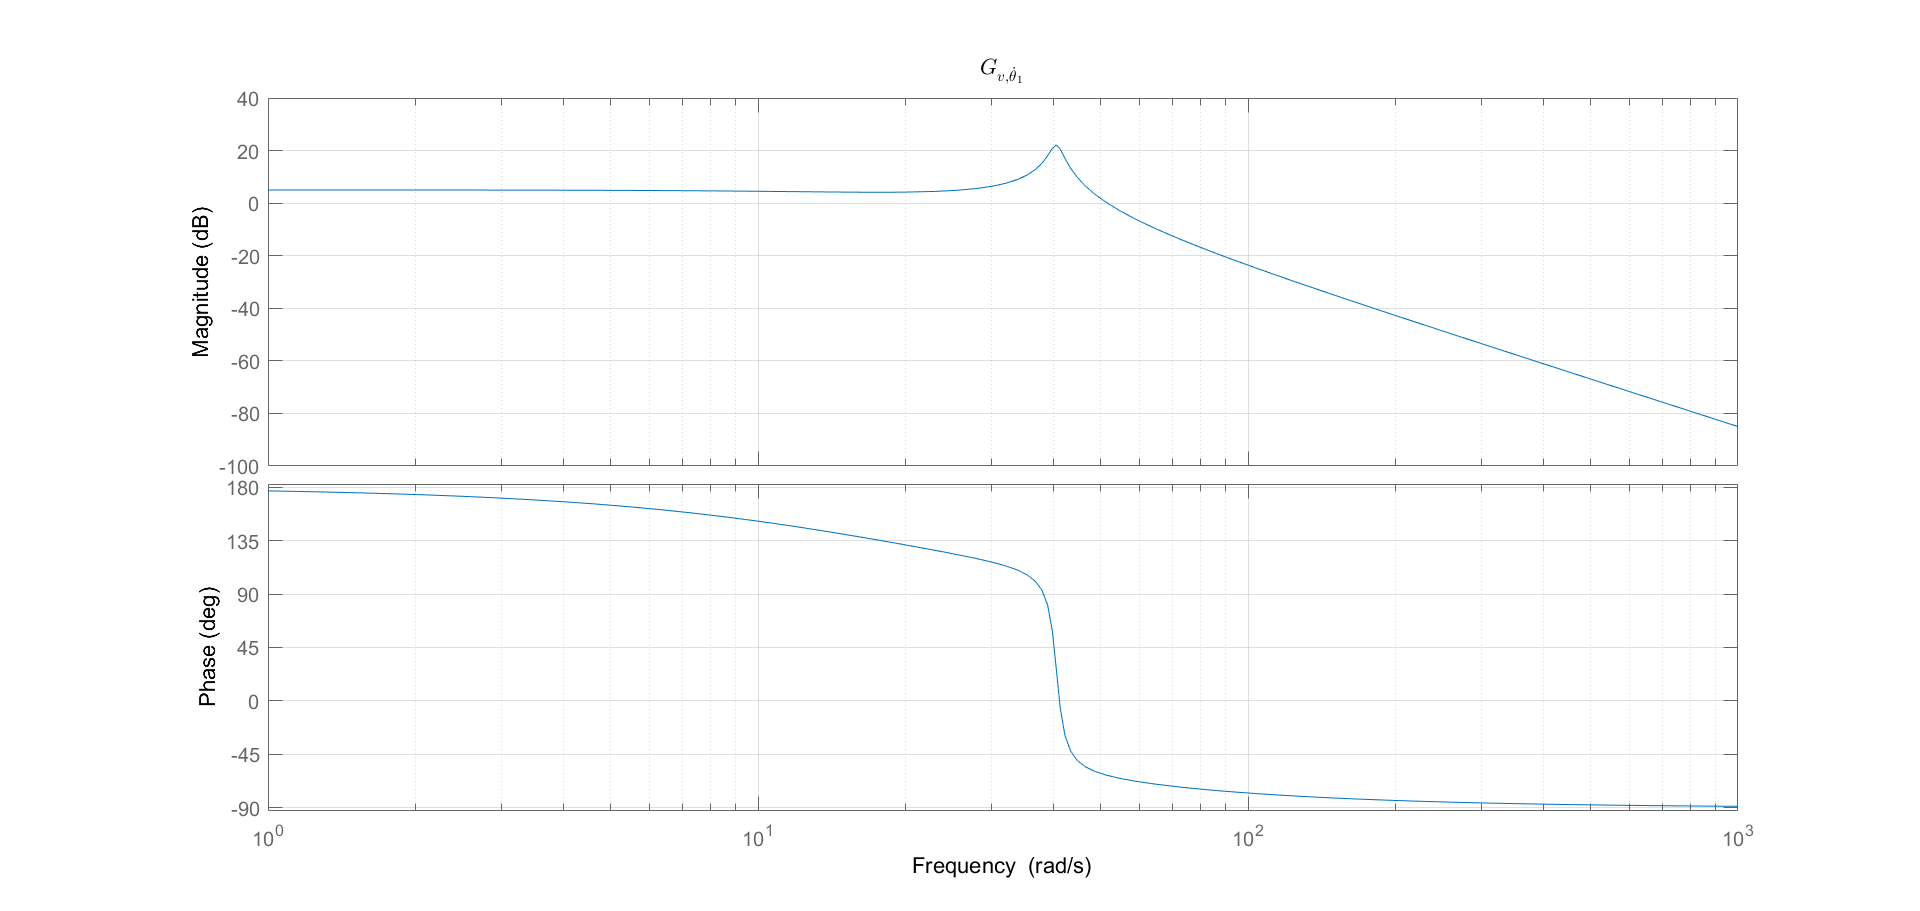
\includegraphics[width=\textwidth]{1Bode_G}
	\end{subfigure}
	\begin{subfigure}{0.4\columnwidth}
		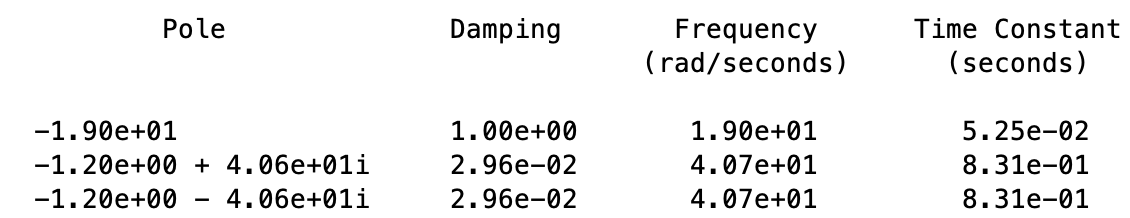
\includegraphics[width=\textwidth]{1Pole_G}
	\end{subfigure}
	\caption{$G_{v, \dot \theta_1}(s)$}
	\label{fig:G(s)1dof}
\end{figure*}

It is possible to notice, in \cref{fig:G(s)1dof}, that there is a couple of complex conjugated poles with low damping coefficient. The proposed solution is to apply a notch filter, thanks to which it is possible to delete these poles and substitute them with a couple of complex conjugated poles at the same frequency, but with a damping coefficient equal to~$0.72$. It has been decided not to alter too much the behavior of the plant to avoid too aggressive control actions, for this reason notch poles haven't been imposed as real poles or as high frequency poles.

\begin{figure*}[h]
	\centering
	\begin{subfigure}{0.47\columnwidth}
		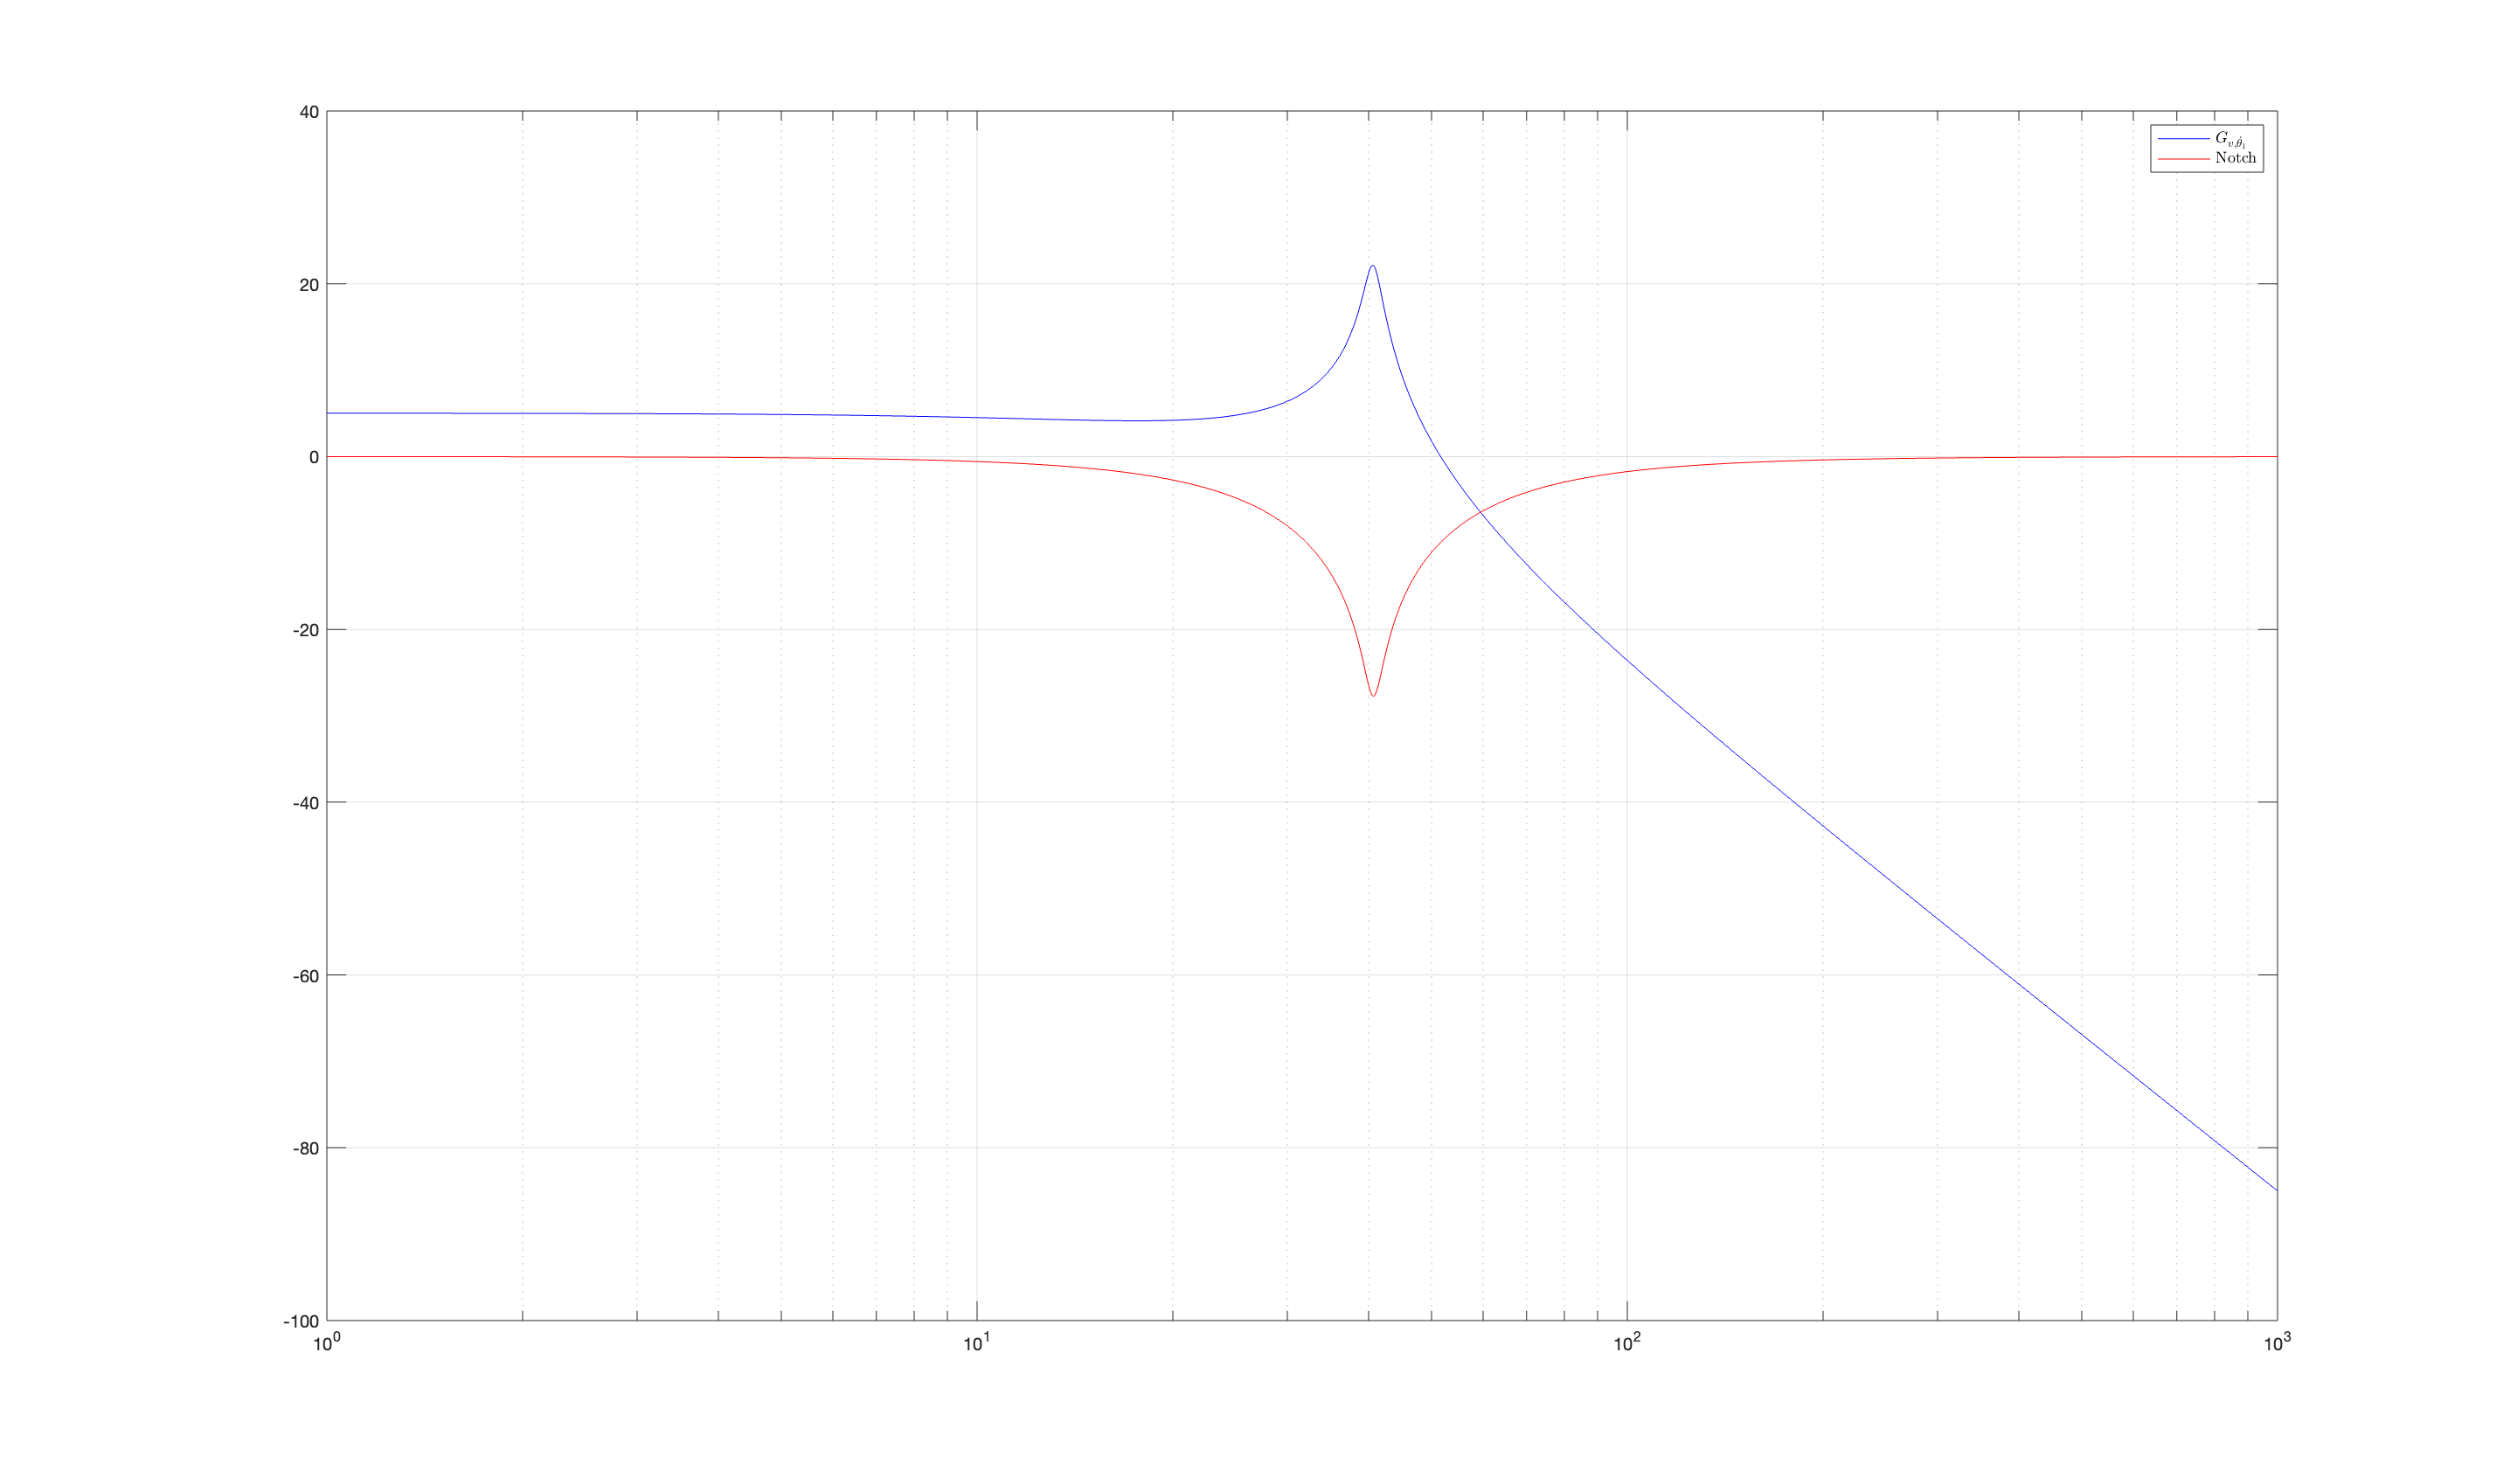
\includegraphics[width=\textwidth]{1Nf_G}
		\subcaption{$N_f(s)$ and $G(s)$}
	\end{subfigure}
	\begin{subfigure}{0.47\columnwidth}
		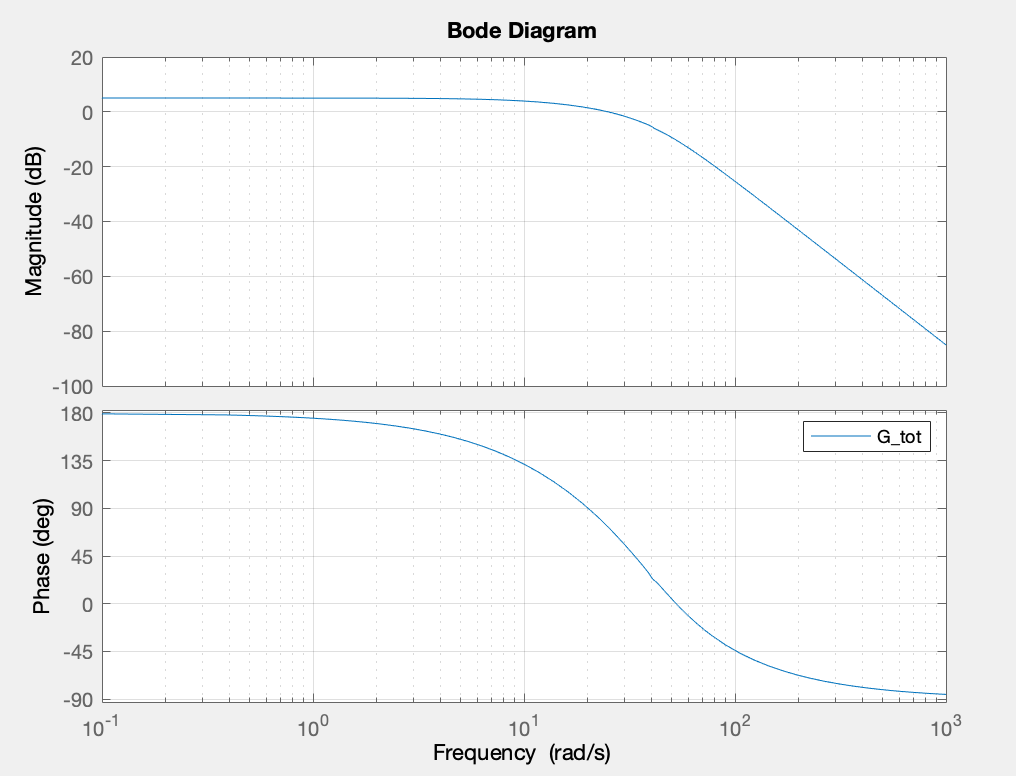
\includegraphics[width=\textwidth]{1_Gtot}
		\subcaption{$G_{tot}(s)$}
	\end{subfigure}
	\caption{Plant $G(s)$ with Notch Filter $N_f(s)$: $G_{tot}(s)$}
	\label{fig:Plant G(s)with Notch Filter1}
\end{figure*}


Applying the notch filter represented in \cref{fig:Plant G(s)with Notch Filter1}(a), the controller now sees the plant $G_{tot}$(s) of \cref{fig:Plant G(s)with Notch Filter1}(b).

\newpage
\subsection{Speed Control Loop}
The selected controller structure is the PI, enriched with an anti-windup structure, that cancels out the real frequency pole at~$19\ rad/s$.
\begin{center}
$ R(s) = -k_v \frac{\frac{s}{19}+1}{s} $,
with \quad
$ k_{v} = \frac{w_{c,v}}{G(0)} $
\end{center}
\begin{figure*}[h]
	\centering
	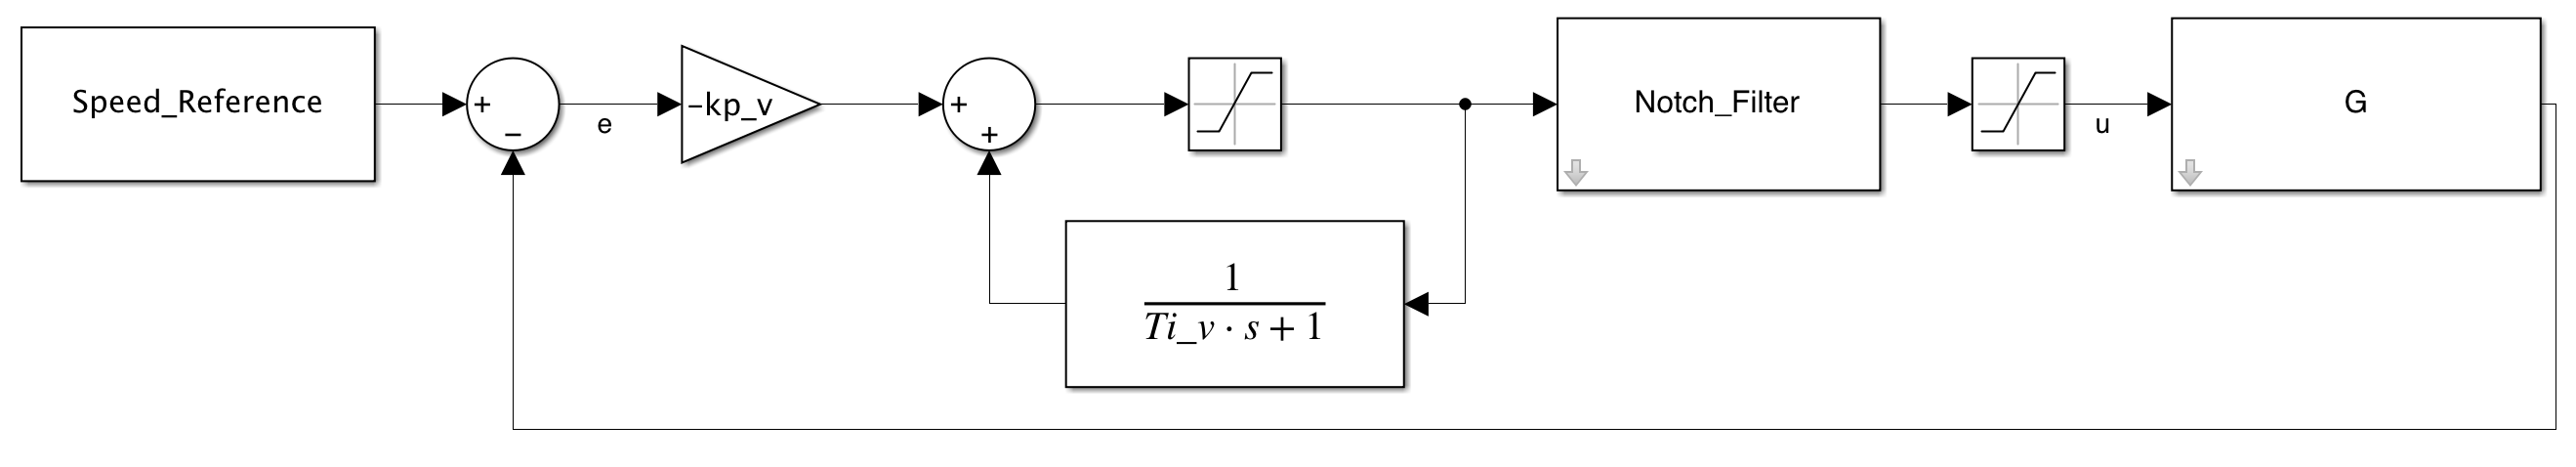
\includegraphics[width=0.8\textwidth]{1dof_PI_scheme}
	\caption{Closed-loop block scheme}
\end{figure*}

\paragraph{Specifications}
The goal of this first controller is to obtain a fast and robust performance. In particular,
\begin{itemize}
	\item settling time: $T_s \leq 0.5\ s$
	\item phase margin: $\phi_m \geq 65\degree$
\end{itemize}

\paragraph{Tuning and simulation}
From now on, $k_v$ will be used as tuning parameter of the PI regulator, while the~$0\ dB$ axis of Bode diagram of speed loop is indicated by~$w_{c,v}$. In order to obtain the desired specifications, many Bode analyses and simulations have been done: here is reported a comparison between step responses with~$k_v=3.5$ and~$k_v=4.5$ (\cref{fig:PI1dof_comparison}).
The only choice that satisfies all the requirements is obtained by imposing~$k_v = 4.5$: open-loop and closed-loop Bode diagrams are shown in \cref{fig:PI1dof_bode}; here, it can be noticed that the cross-over frequency of the open-loop (detected by MATLAB \textit{margin} function) does not perfectly coincide with the closed-loop bandwidth, that will be estimated in \cref{par:1dof_vel_bwEstimation}.
\begin{figure*}[h]
	\centering
	\begin{subfigure}{0.45\columnwidth}
		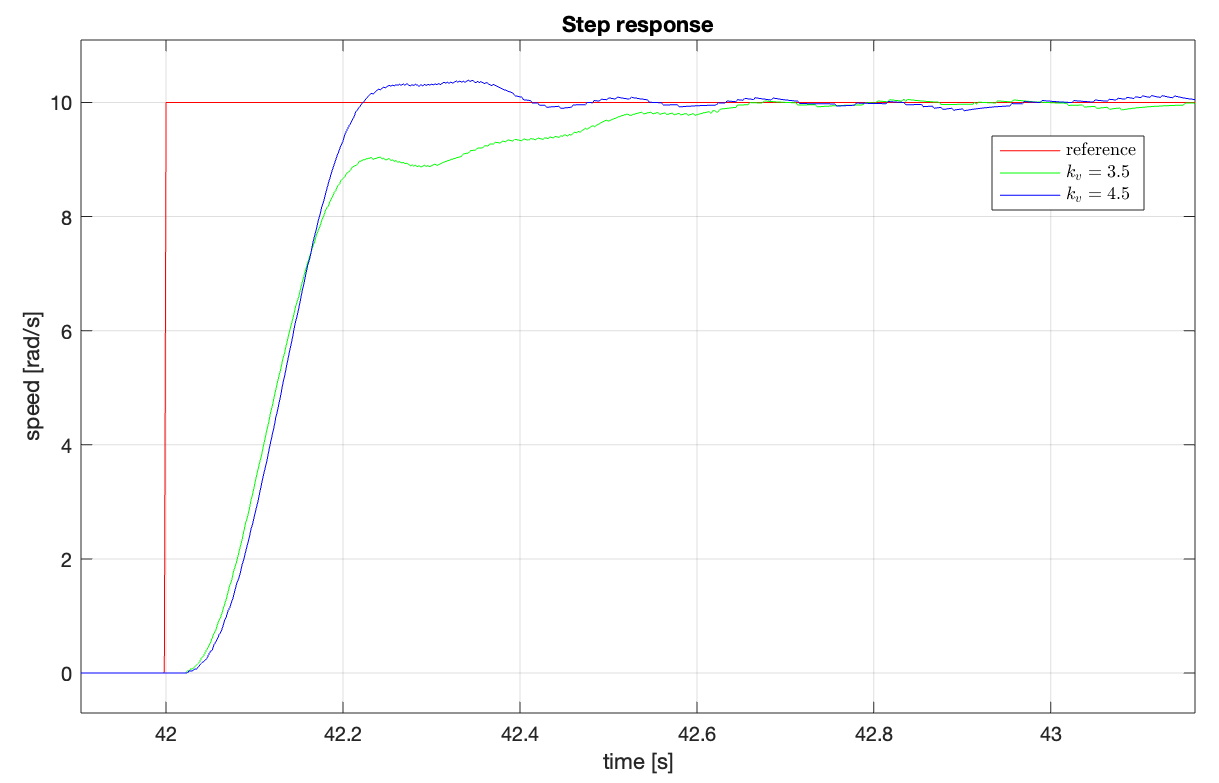
\includegraphics[width=\textwidth]{1dof_step_trials}
		\subcaption{Laboratory data of closed-loop step responses}
		\label{fig:PI1dof_step}
	\end{subfigure}
	\begin{subfigure}{0.45\columnwidth}
		\centering
		\begin{tabular}{|c|cc|}
			\hline
			Results\footnote{Open-loop cross-over frequency~$\omega_{c,v}$, gain margin~$G_m$ and phase margin~$\phi_m$ are obtained theoretically by means of MATLAB. Instead, settling time~$T_s$ is measured through data collected at the laboratory.} & $k_v=3.5$ & $k_v=4.5$ \\
			\hline
			$\omega_{c,v}\ [rad/s]$ & $6.24$ & $8.01$ \\
			$G_m\ [dB]$ & $19$ & $16.8$ \\
			$\phi_m\ [deg]$ & $77.3$ & $73.6$ \\
			\hline
			$T_s\ [s]$ & $0.65$ & $0.40$ \\
			\hline
		\end{tabular}
		\subcaption{Table of theoretical results, $k_v = 3.5$ and $k_v = 4.5$ cases}
	\end{subfigure}
	\caption{Comparisons between $k_v = 3.5$ and $k_v = 4.5$ cases}
	\label{fig:PI1dof_comparison}
	\begin{subfigure}{0.45\columnwidth}
		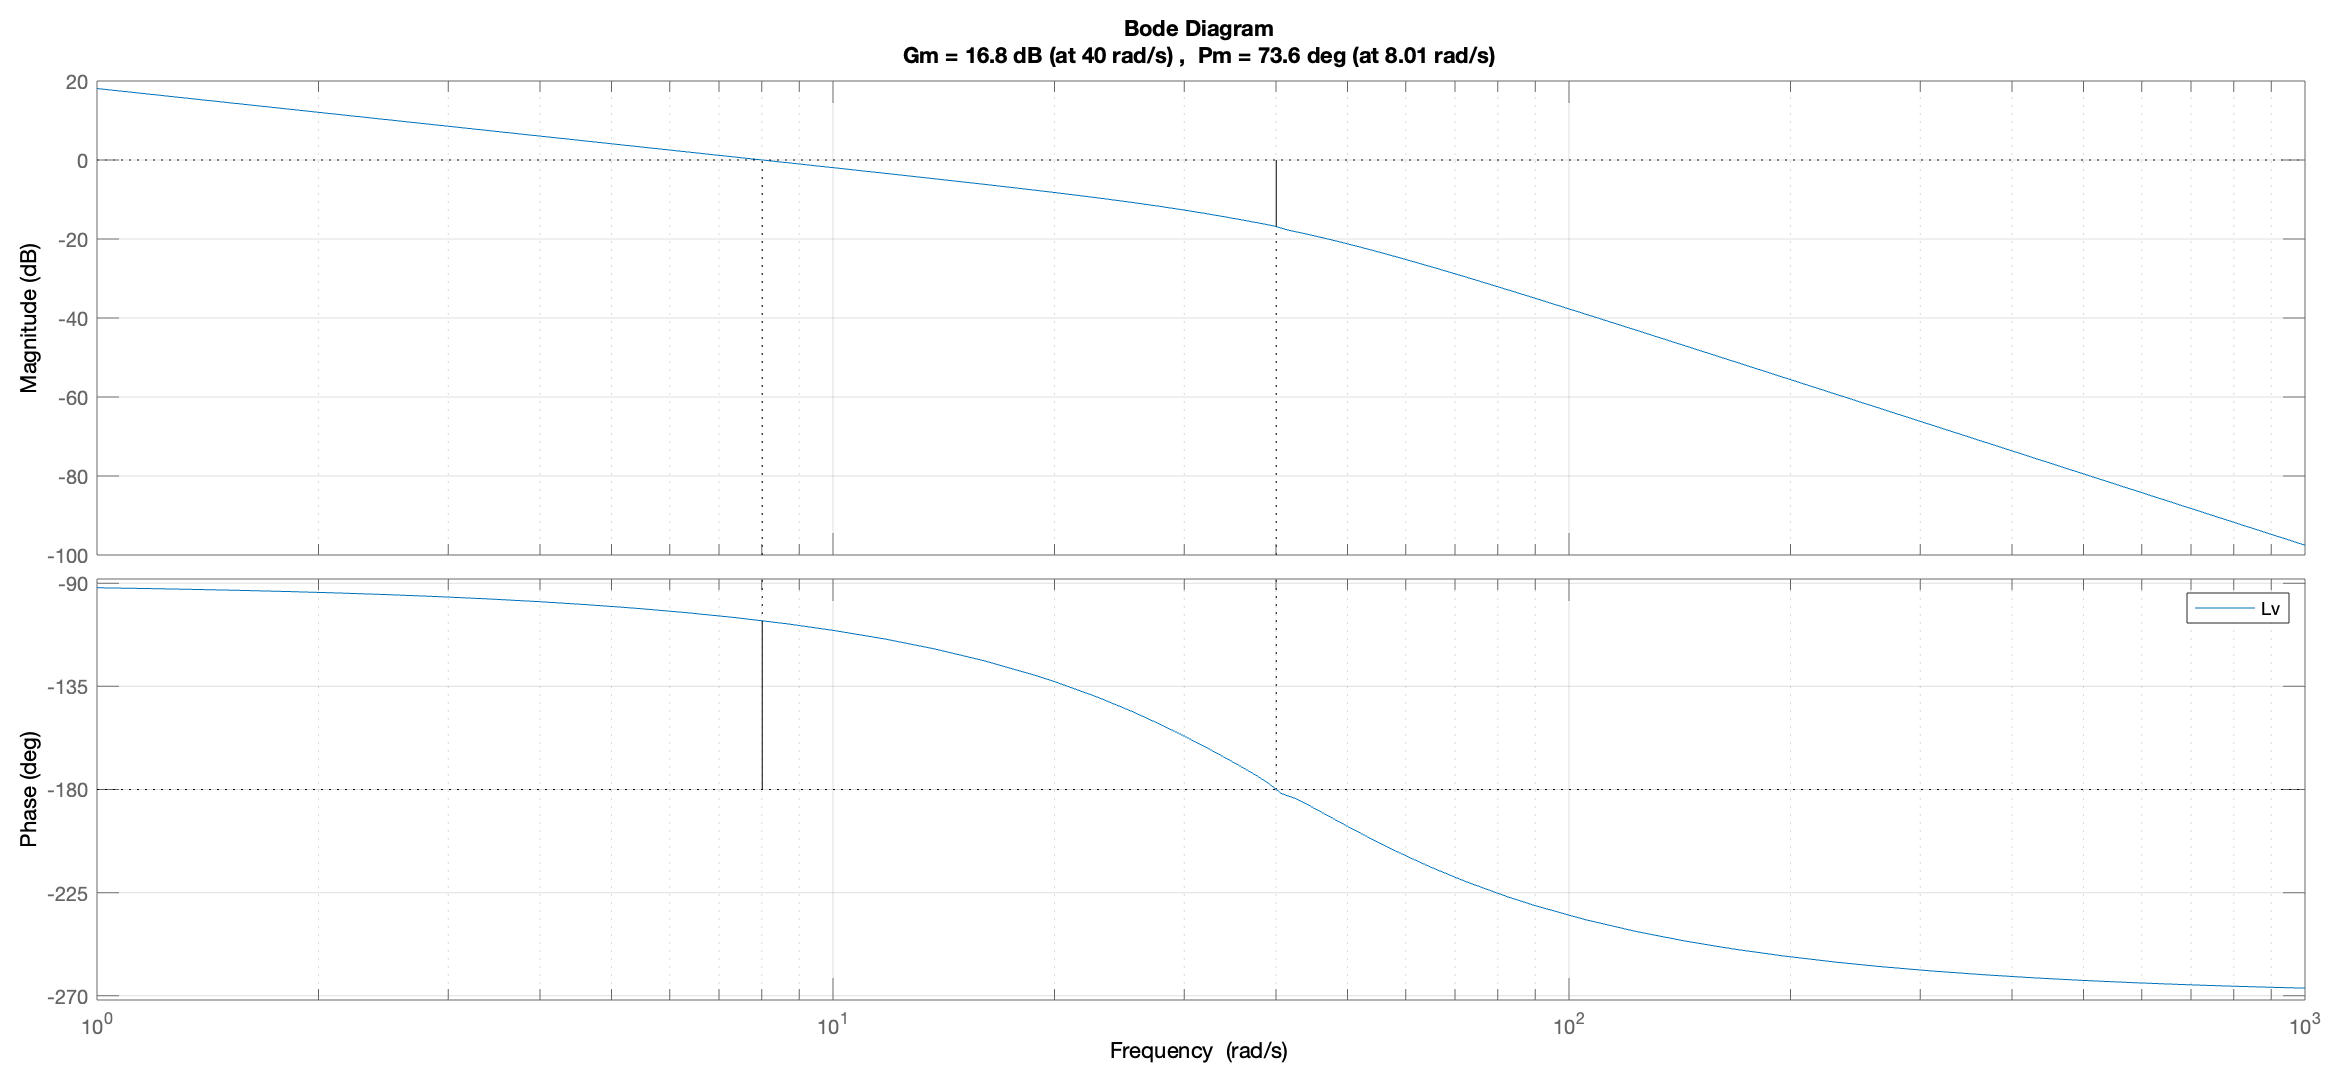
\includegraphics[width=\textwidth]{openloop_margin_speed_1dof}
		\subcaption{Open-loop}
		\label{fig:PI1dof_bode_openLoop}
	\end{subfigure}
	\begin{subfigure}{0.45\columnwidth}
		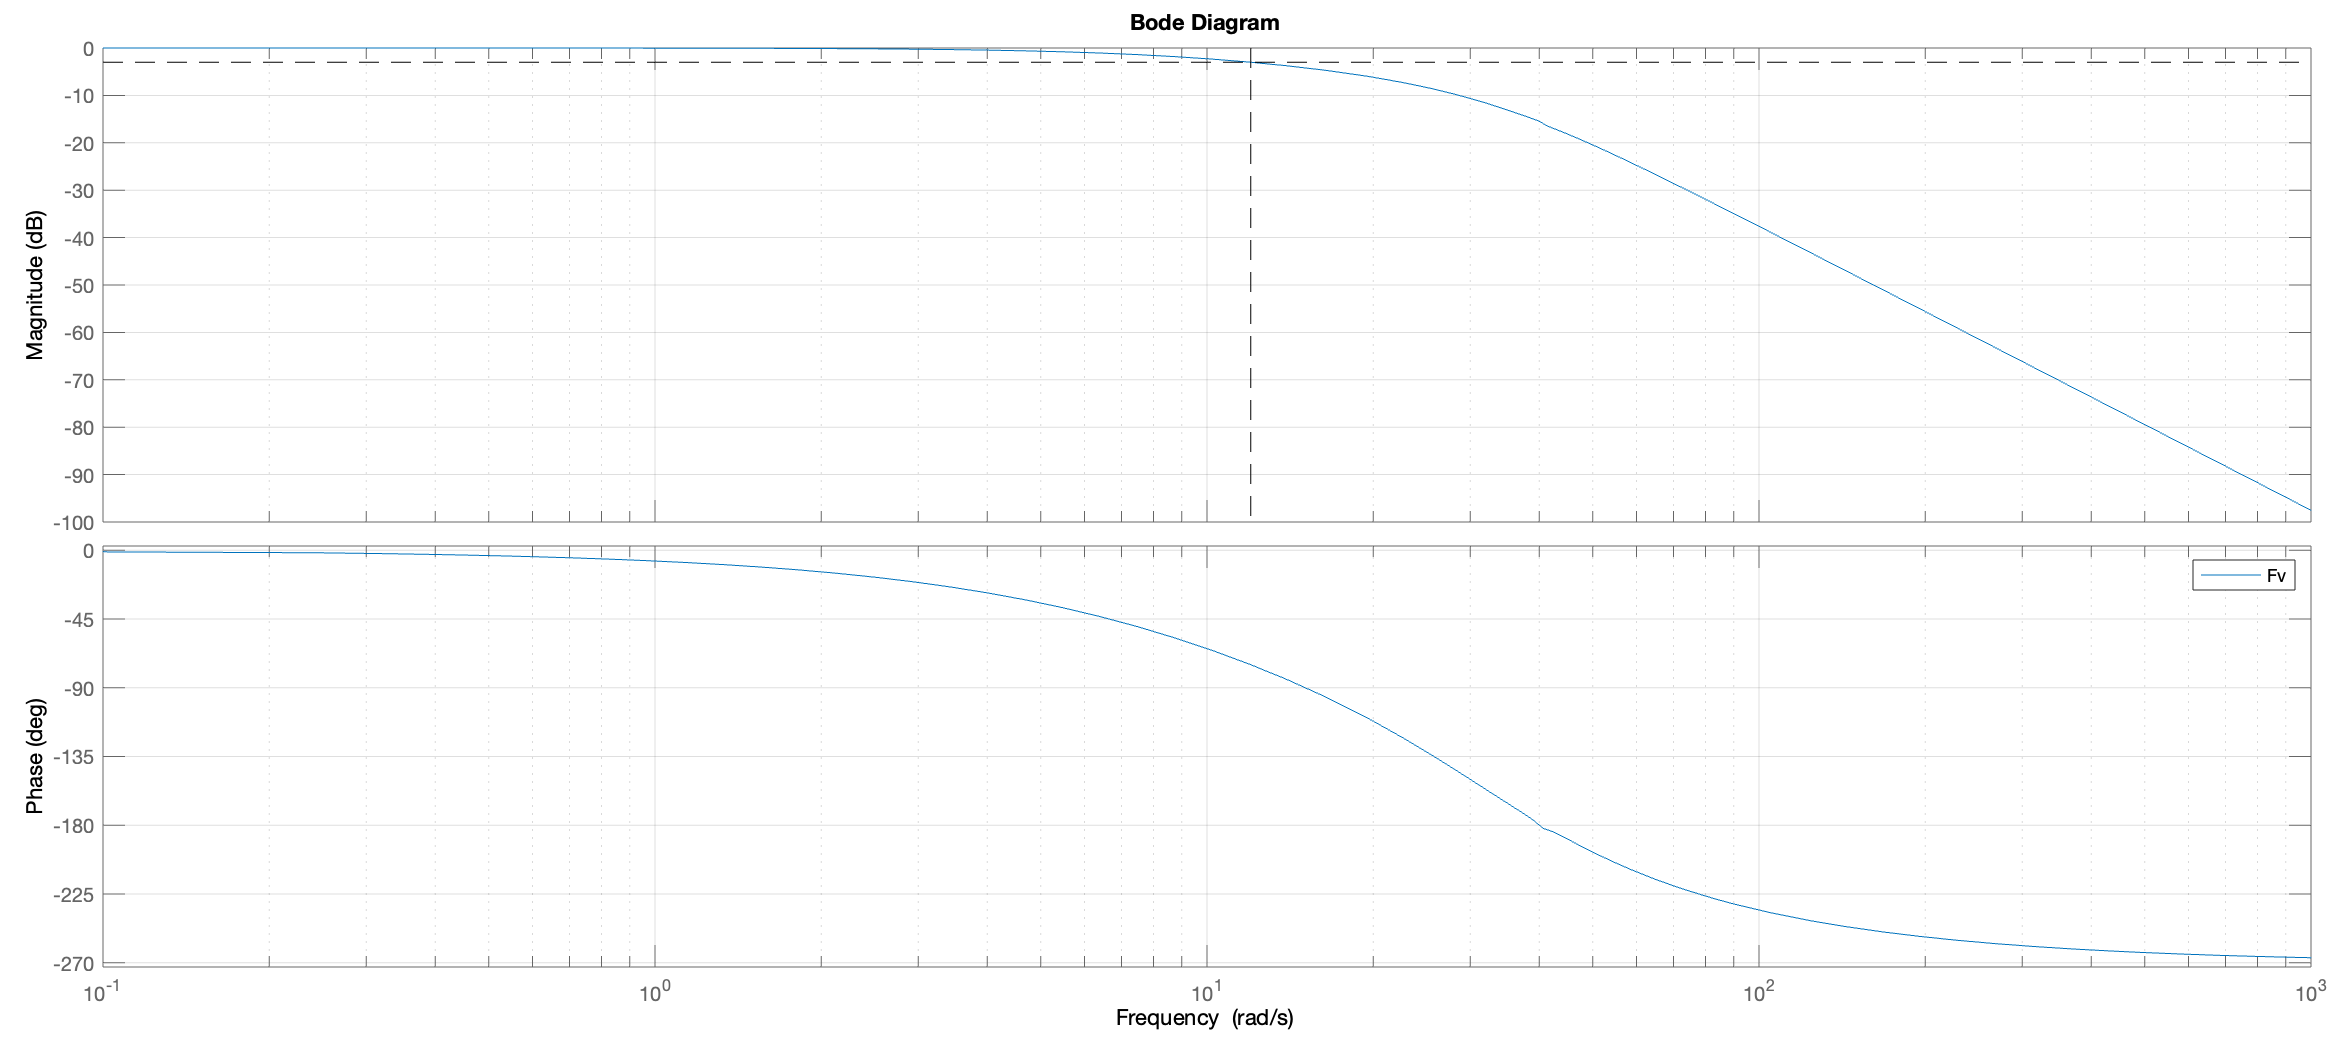
\includegraphics[width=\textwidth]{closedloop_bode_speed_1dof}
		\subcaption{Closed-loop}
		\label{fig:PI1dof_bode_closedLoop}
	\end{subfigure}
	\caption{Bode diagrams with $k_v = 4.5$}
	\label{fig:PI1dof_bode}
\end{figure*}

\paragraph{Performance analysis}
To test the chosen controller, one of the worst case scenarios has been applied, that is the step from~$-17\ rad/s$ to~$17\ rad/s$, and then a smaller step of~$10\ rad/s$. The first one allows to asses the voltage saturation in the worst case, while the second one can be representative of the transient for an ordinary step.
In \cref{fig:PI with 4.5} is shown the comparison between the simulation and the data collected in the laboratory on the real system.
\begin{figure*}[h]
	\centering
	\begin{subfigure}{0.45\columnwidth}
		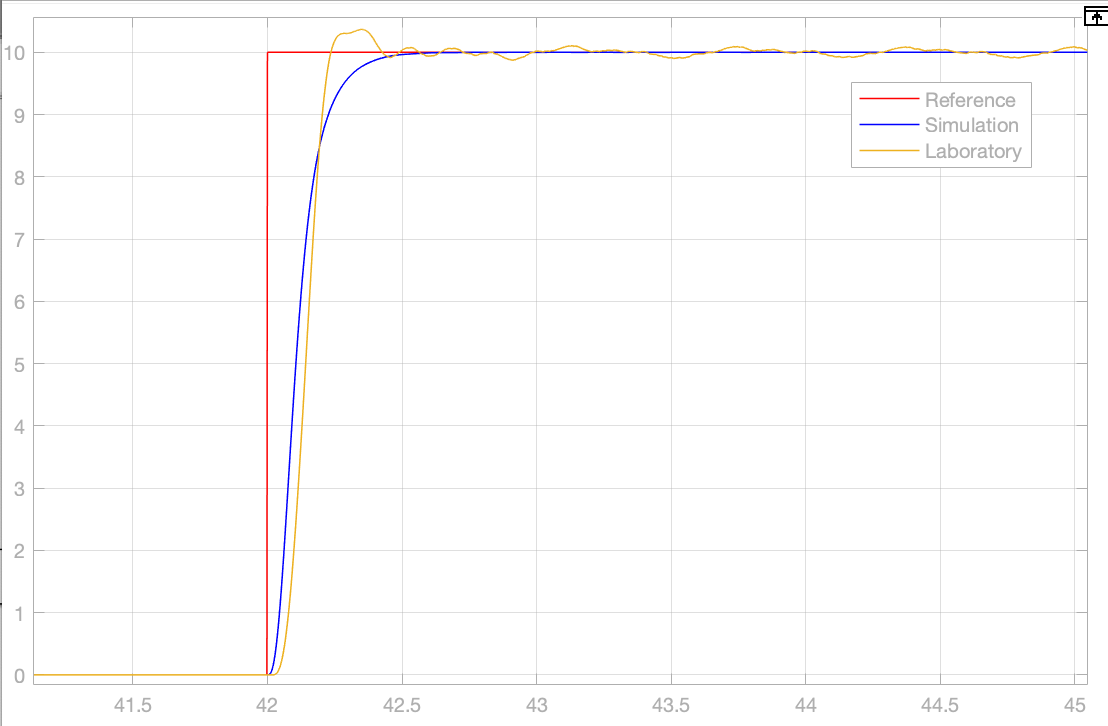
\includegraphics[width=\textwidth]{1_step10}
		\subcaption{Step of $10\ rad/s$}
		\label{fig:PI with 4.5 step 10}
	\end{subfigure}
	\begin{subfigure}{0.45\columnwidth}
		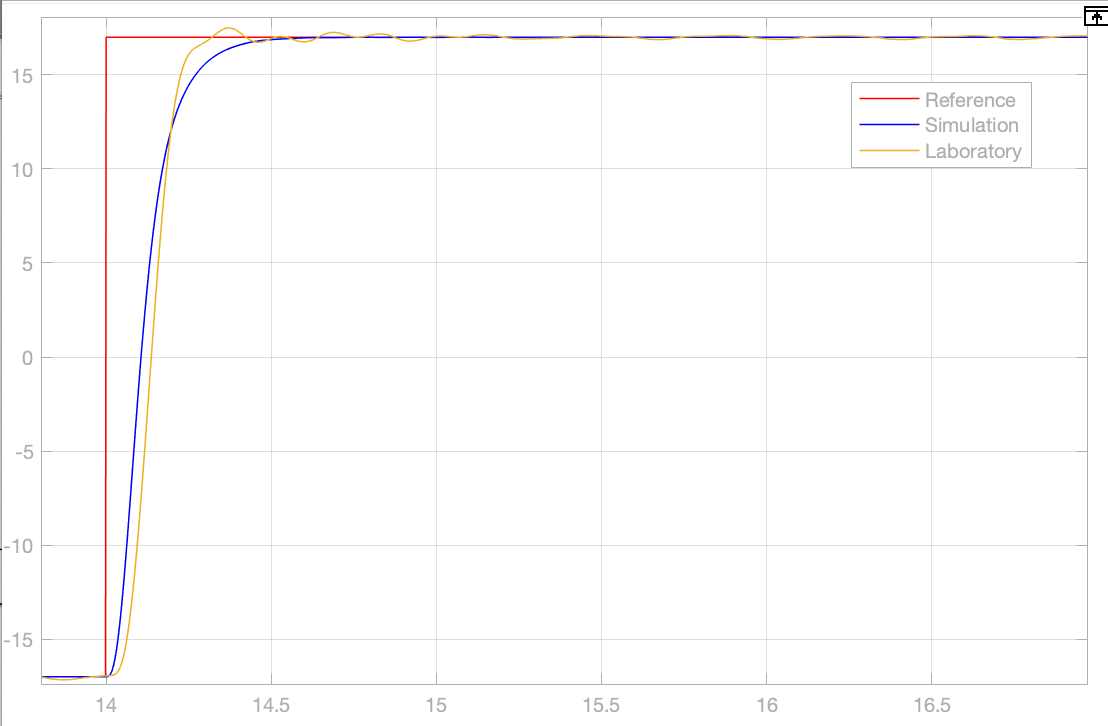
\includegraphics[width=\textwidth]{1_step17}
		\subcaption{Step of $34\ rad/s$}
	\end{subfigure}
	\newline
	\begin{subfigure}{0.45\columnwidth}
		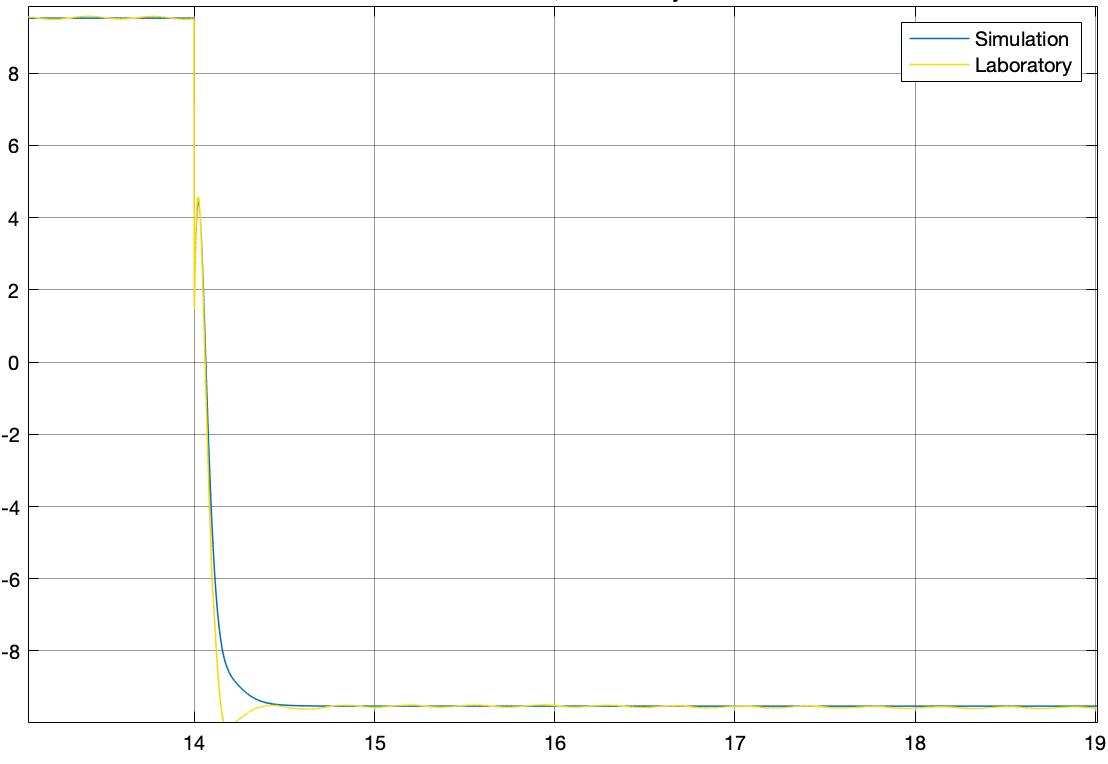
\includegraphics[width=\textwidth]{1_volt17}
		\subcaption{Voltage related to a step of $34\ rad/s$}
	\end{subfigure}
	\caption{Speed control loop with $k_{v}=4.5$}
	\label{fig:PI with 4.5}
\end{figure*}
\subparagraph{Overshoot and phase margin}
In the experimental data, an overshoot appears (in \cref{fig:PI with 4.5 step 10} the reference step is not sufficiently high to cause voltage saturation). This behavior is due to a lower phase margin of the real system, caused by a wrong estimation of the dominant pole, whose frequency might be actually lower than~$19\ rad/s$. \\
This issue allows to compute the phase margin: through the overshoot height percentage ($S_\% = \frac{0.4\ rad/s}{10\ rad/s} = 4\%$), it is possible to compute the system approximation damping~$\xi$ and, so, the phase margin~$\phi_m$ by means of the following formulas.
\begin{equation}
	S_\% = 100\ e^{\frac{-\pi\xi}{\sqrt{1-\xi^2}}} ,
	\qquad
	\phi_m = \frac{180\degree}{\pi} \arctan \Biggl( \frac{2\xi}{\sqrt{-2\xi^2 + \sqrt{1+4\xi^4} }} \Biggr)
	\label{eq:phase_margin_compute}
\end{equation}
The obtained value is~$\phi_m = 66.2 \degree$, that is considered satisfactory according to our initial specifications.

\subparagraph{Oscillations}
A resonance uncertainty is observable through the small oscillations at the end of the transient, which are not well compensated by the notch filter. \\
Another aspect that has to be considered is the presence of oscillations at steady-state. Their frequencies are equal to the speed, then a possible explanation can be a change of the dynamic friction coefficient value along the revolution. As a matter of fact, this undesired behavior can be neglected, since the amplitude of the above-mentioned oscillations is very small. In case is necessary to attenuate them, the bandwidth of the loop should be increased to counteract them on time. By using just a PI as controller this is not possible, because increasing the cutting frequency would result in lower phase margin and significant oscillations to the step response, that cannot be accepted. \\
To avoid this behavior to steps in the reference signals, a solution could be placing a low-pass pre-filter on the reference signal. In this way, a step on the speed reference would result in a smoother reference signal and smaller oscillations will arise. This solution is analyzed with more details in the \twodof\ case, where these oscillations at the steady-state cannot be neglected.

\paragraph{Bandwidth estimation}
\label{par:1dof_vel_bwEstimation}
In \cref{fig:sinesweep_PI_1dof} and \cref{fig:Ramp1dof} are shown the responses of the closed-loop system to a sine-sweep, experiment that allows to evaluate its bandwidth, and to a ramp reference with a decreasing slope, that permits to asses the range of reachable speed set-points (especially for what concerns the low speeds). \\
The analysis of both step and closed-loop sine-sweep responses, respectively \cref{fig:PI with 4.5} and \cref{fig:sinesweep_PI_1dof}, reveal that simulations do not follow exactly the data collected in the laboratory. This difference is caused by a non perfect identification of the real system. Indeed, an estimation of the bandwidth from the sine-sweep experiment is performed, two different cross-over frequencies are obtained: the simulation places it around~$11.5\ rad/s$ and the real system one appears to be around~$14.9\ rad/s$. These values have been computed according to the theory, for which the attenuation at the cutting frequency is~$-3\ dB$. \\
It can be noticed that a small resonance occurs around the cross-over frequency of the real system: a phase margin smaller that~$70 \degree$ can lead to this behavior. \\
Moreover, it cannot be neglected the fact that this is a speed controller. Speed measurement is obtained through the derivation of the position of the encoder. Thus, these bandwidth values are not fully reliable because of uncertainty in measurement.
\begin{figure*}[h]
	\centering
	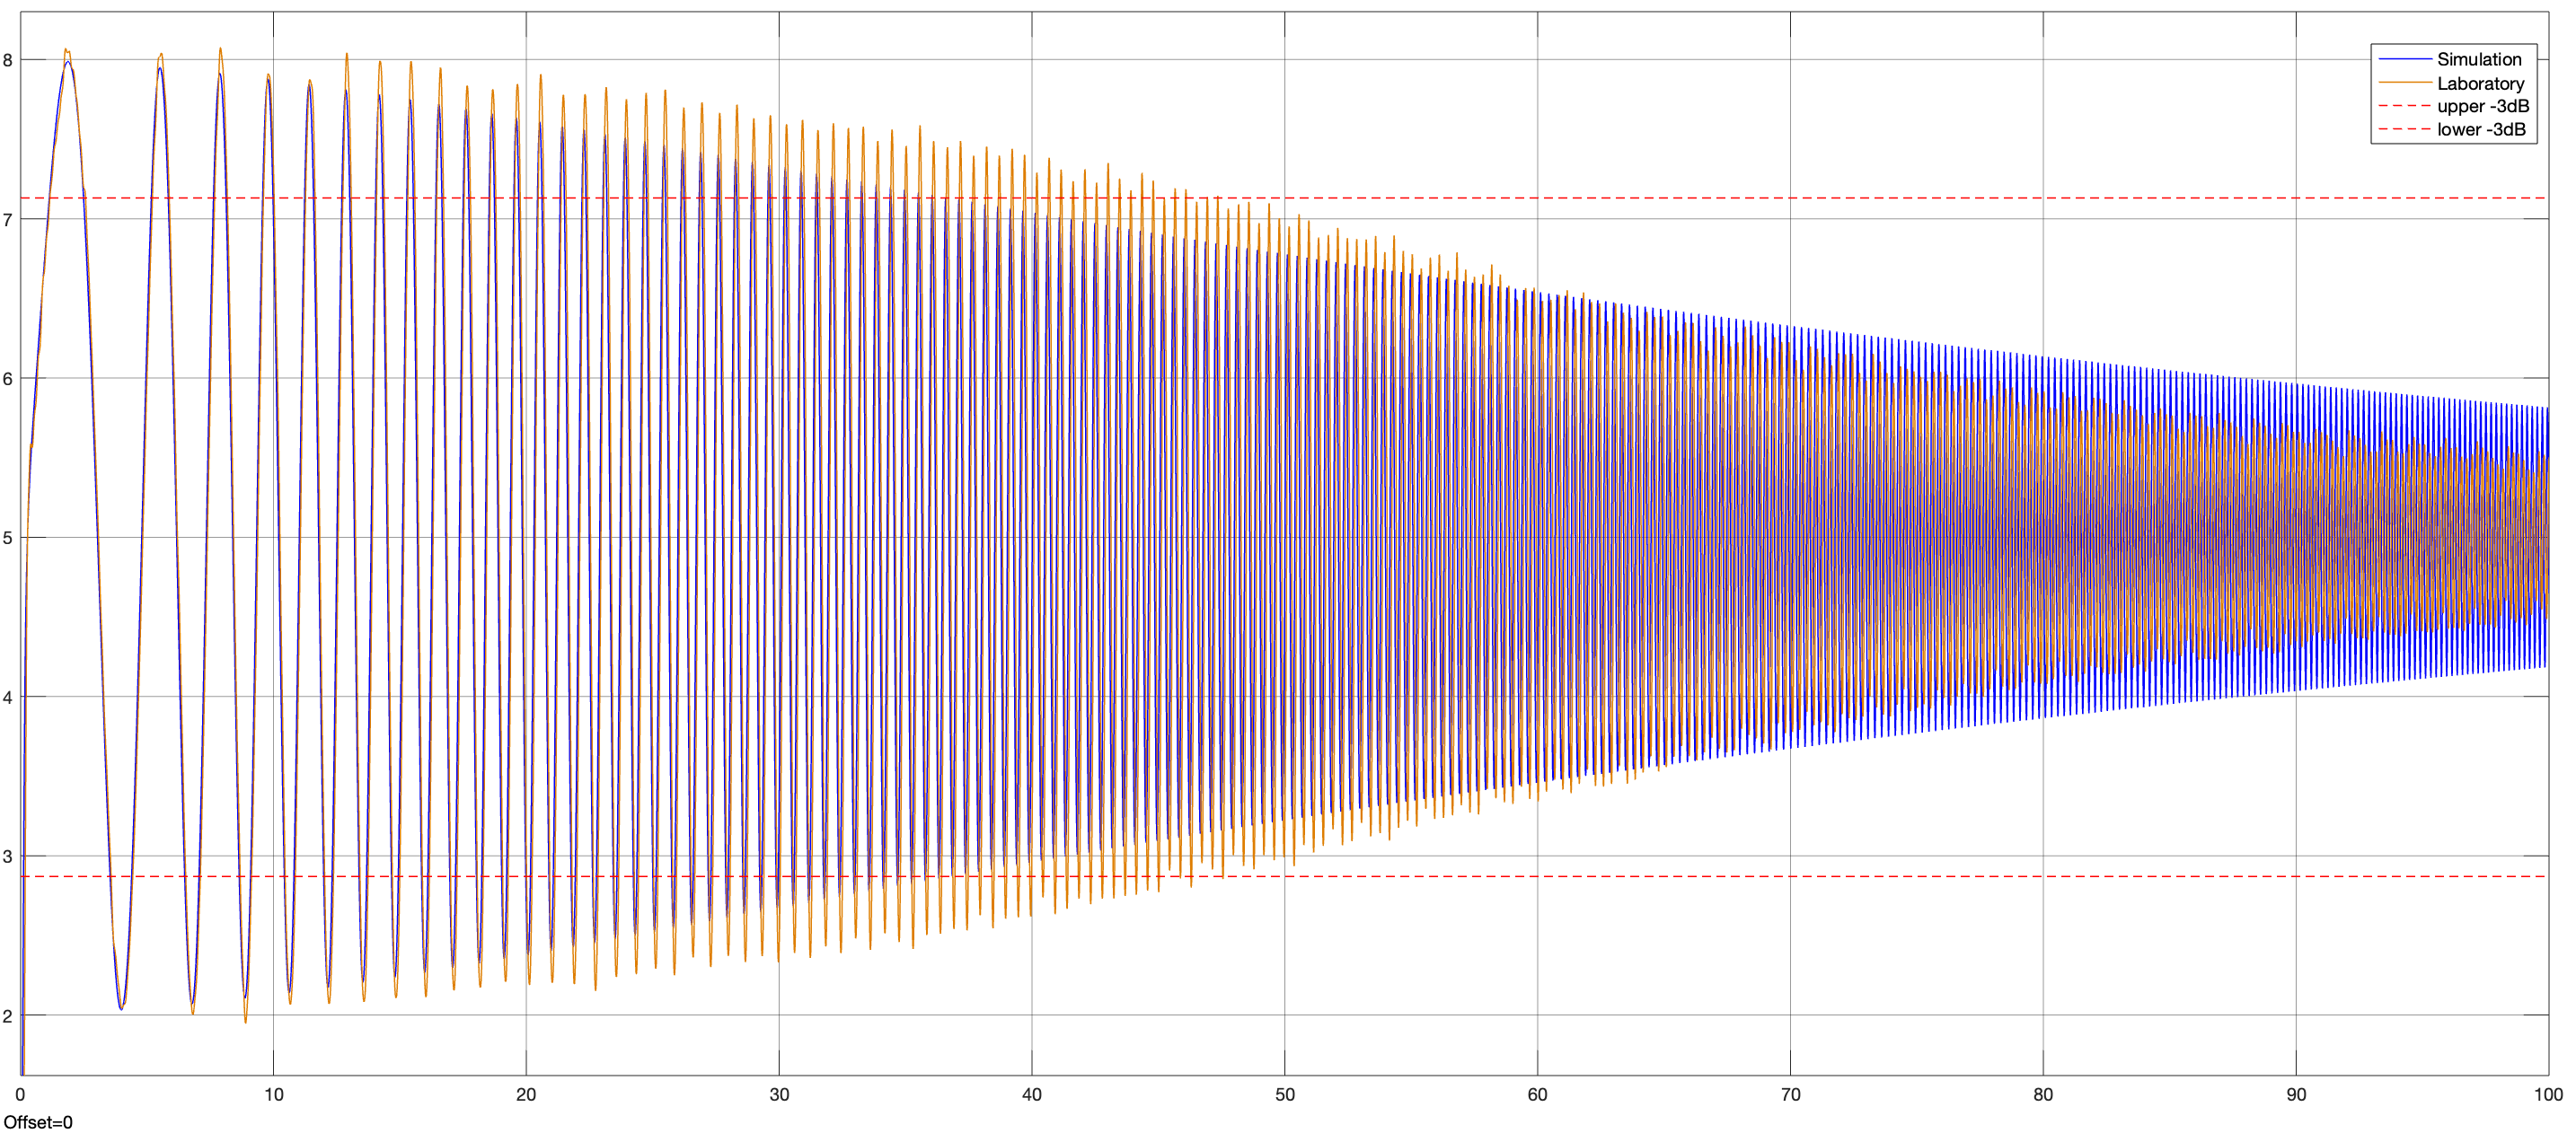
\includegraphics[width=0.9\columnwidth]{Sine1dof}
	\caption{Sineweep experiment from $0.1\ Hz$ to $10\ Hz$ in $100\ s$}
	\label{fig:sinesweep_PI_1dof}
\end{figure*}
\begin{figure*}[h]
	\centering
	\begin{subfigure}{0.4\columnwidth}
		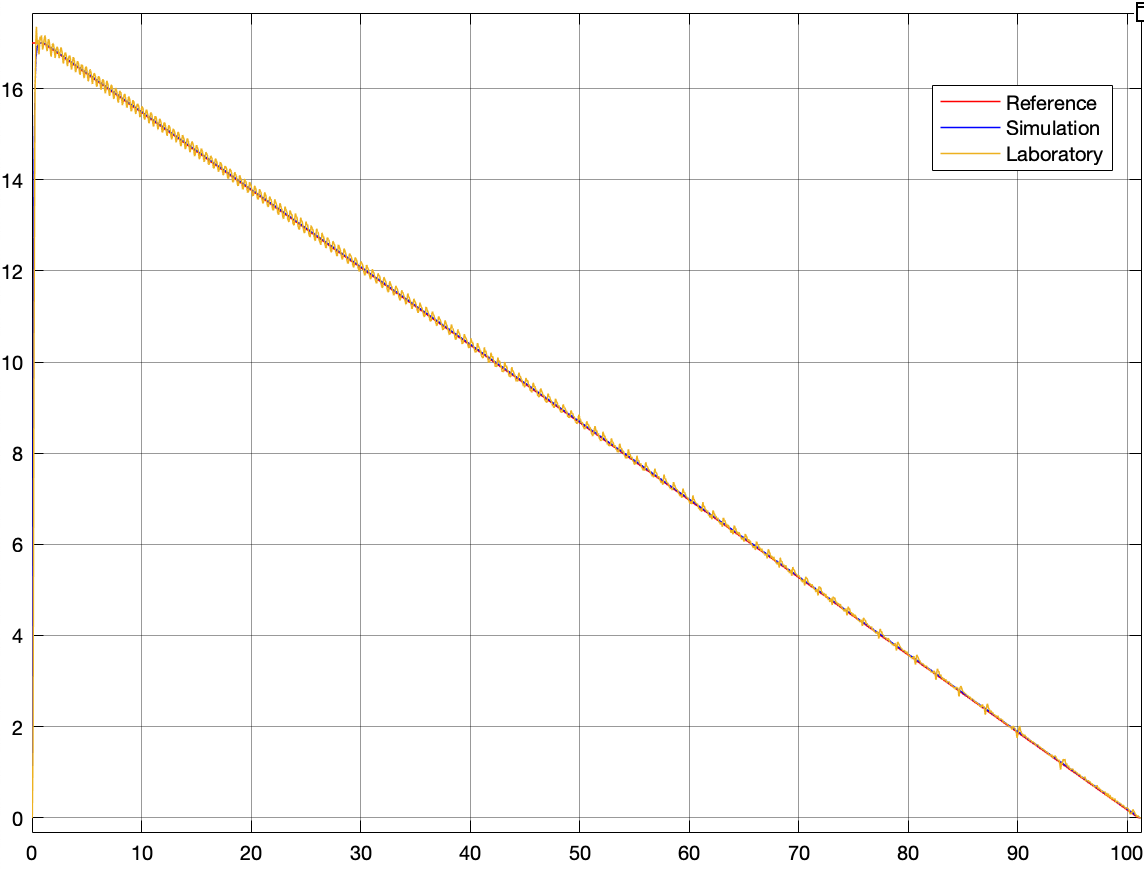
\includegraphics[width=\textwidth]{Ramp1dofa}
		\subcaption{Entire experiment}
	\end{subfigure}
	\begin{subfigure}{0.4\columnwidth}
		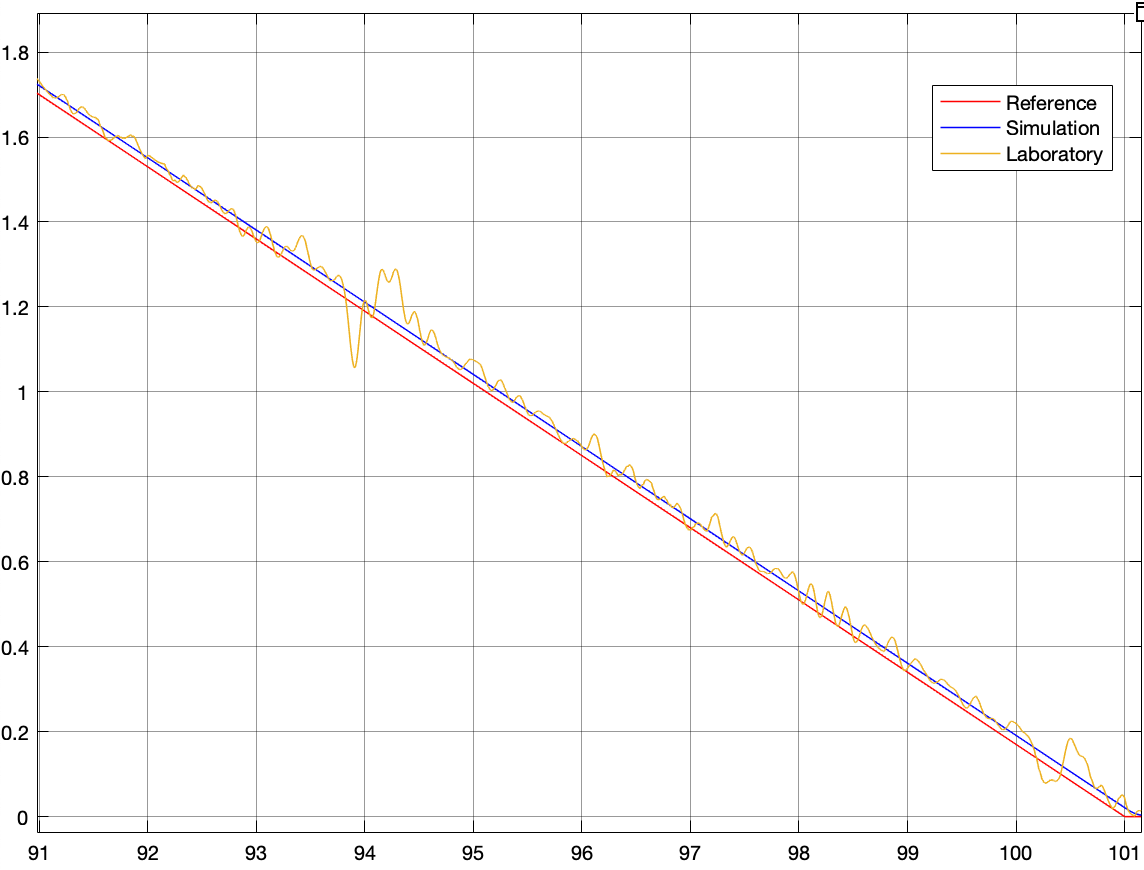
\includegraphics[width=\textwidth]{Ramp1dofb}
		\subcaption{Detail at low speed}
	\end{subfigure}
	\caption{Ramp experiment from $17\ rad/s$ to $0\ rad/s$ in $100\ s$}
	\label{fig:Ramp1dof}
\end{figure*}

Thanks to the ramp experiment, it has been verified that this regulator can control the system even at very low speed. This is a very satisfactory result, because of the wide range of reachable references, which go from~$-17.5\ rad/s$ to~$-0.3\ rad/s$ and from~$0.3\ rad/s$ to~$17.5\ rad/s$.

\subsection{Position Control Loop}
To control the position, different techniques have been considered: direct P and PI controllers on the mass position error have been taken into account. Since the speed control loop has highlighted some uncertainties on the model, a cascade control is useful for disturbances rejection and to face uncertainties.
\begin{figure*}[h]
	\centering
	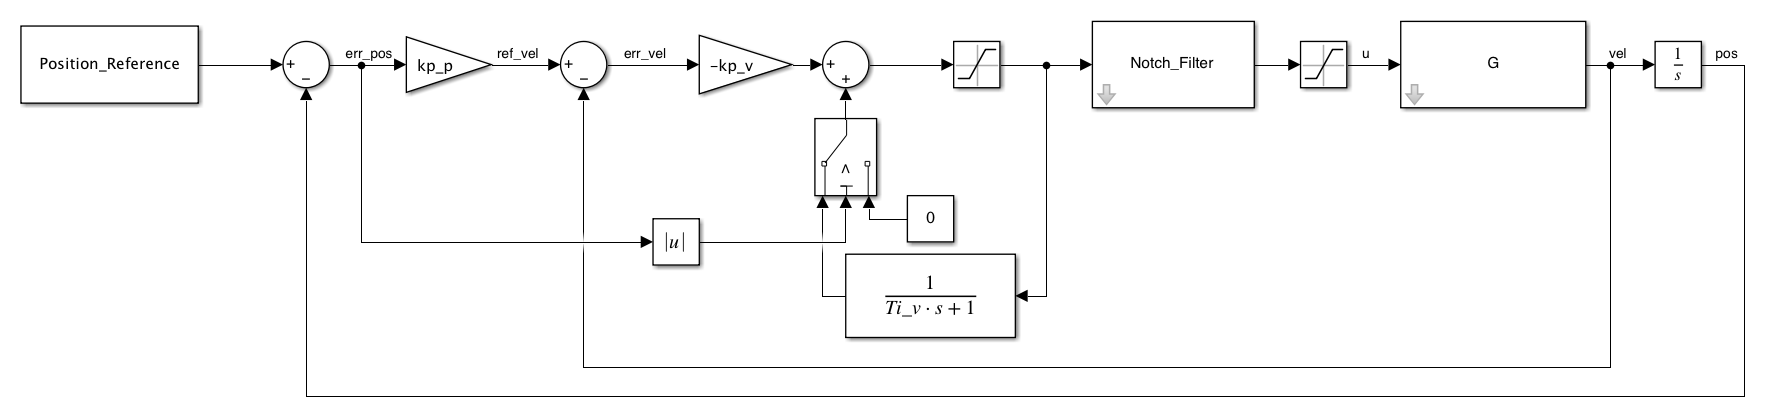
\includegraphics[width=0.8\textwidth]{1dof_P_scheme}
	\caption{Closed-loop block scheme}
\end{figure*}

\paragraph{Tuning and simulation}
The inner loop controls the speed, whereas the outer one the position. For the first loop, it is used the same PI structure as the previous section, while the position is regulated by using a proportional controller. It is important to remark that the cutting frequency of the position and the speed one must be far enough (about one decade) to ensure the frequency decoupling of the two loops. As consequence, if it is maintained the cutting frequency of the speed loop as decided before ($k_v=4.5$ that corresponds to a bandwidth of~$17\ rad/s$, as estimated in the sine-sweep in \cref{fig:sinesweep_PI_1dof}), a first possible solution is reached by setting the position cutting frequency equal to~$1.7\ rad/s$; however, this solution seems to be extremely slow (only simulation is shown in \cref{fig:P1dof_step}, without experimental data). \\

To overcome this problem, the ratio between the speed cutting frequency and the position one can be pushed up to~$20\ \%$. In this scenario, the proportional gain can be fixed in order to have a higher bandwidth: firstly~$k_p = 2\ rad/s$ and, then, also~$k_p = 3.5\ rad/s$.
In \cref{fig:P1dof_step} all these three cases are compared.
\begin{figure*}[h]
	\centering
	\begin{subfigure}{0.45\columnwidth}
		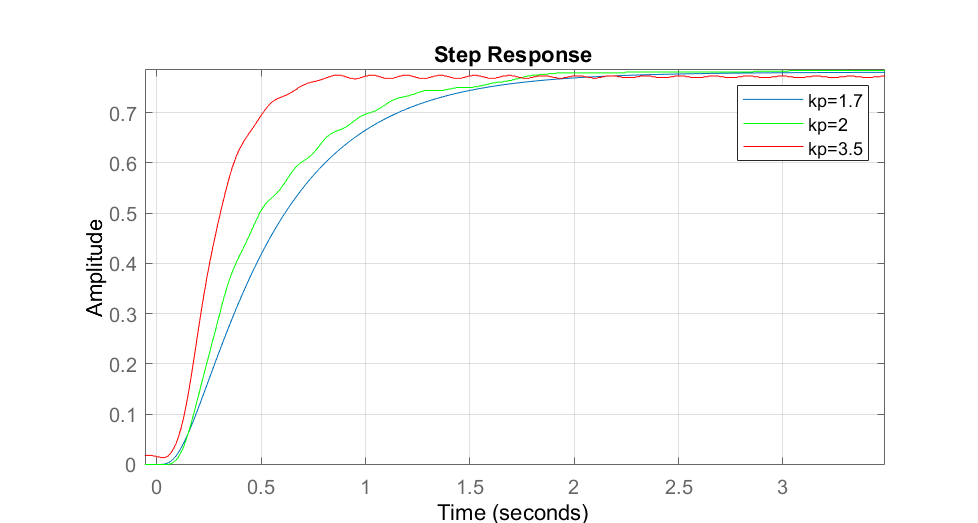
\includegraphics[width=\textwidth]{1dof_P_comparison}
		\subcaption{Closed-loop step responses}
		\label{fig:P1dof_step}
	\end{subfigure}
	\begin{subfigure}{0.45\columnwidth}
		\begin{tabular}{|c|ccc|}
			\hline
			Results\footnote{Gain margin~$G_m$ and phase margin~$\phi_m$ are obtained theoretically by means of MATLAB. Instead, settling time~$T_s$ is measured through data collected at the laboratory.} & $k_p=1.7$ & $k_p=2$ & $k_p=3.5$ \\
			\hline
			$G_m\ [dB]$ & $23.2$ & $21.7$ & $16.9$ \\
			$\phi_m\ [deg]$ & $78.0$ & $76.0$ & $66.3$ \\
			\hline
			$T_s\ [s]$ & $2.30$ & $1.80$ & $0.75$ \\
			\hline
		\end{tabular}
	\end{subfigure}
	\caption{Comparisons between $k_p=1.7$, $k_p=2$ and $k_p=3.5$ cases}
	\label{fig:Bode and Step P 1dof comparison}
\end{figure*}
The last case is certainly the fastest one, so it is considered the best solution reached so far. \\
However, small oscillations occur after the end of the transient; initially, we thought that those were caused by the coupling of speed and position control loops: this suggested us to not speed up the controller with a higher proportional gain, in order to avoid greater oscillations. Spending more time thinking about this problem allowed us to deduce that the previous hypothesis was wrong. A more reasonable explanation attributes the cause of these oscillation to the switch of integrator (explained later on) in the inner loop; so actually, following this reasoning, a faster system could have been obtained. \\

Definitely, the~$k_p = 3.5\ rad/s$ tuning has been chosen, at that time, as the best solution. Bode diagrams of open-loop and closed-loop are reported in \cref{fig:Bode P 3.5}; here, as explained in the speed control loop tuning, the cross-over frequency detected by MATLAB does not perfectly coincides with the bandwidth of the closed-loop.
\begin{figure*}[h]
	\centering
	\begin{subfigure}{0.45\columnwidth}
		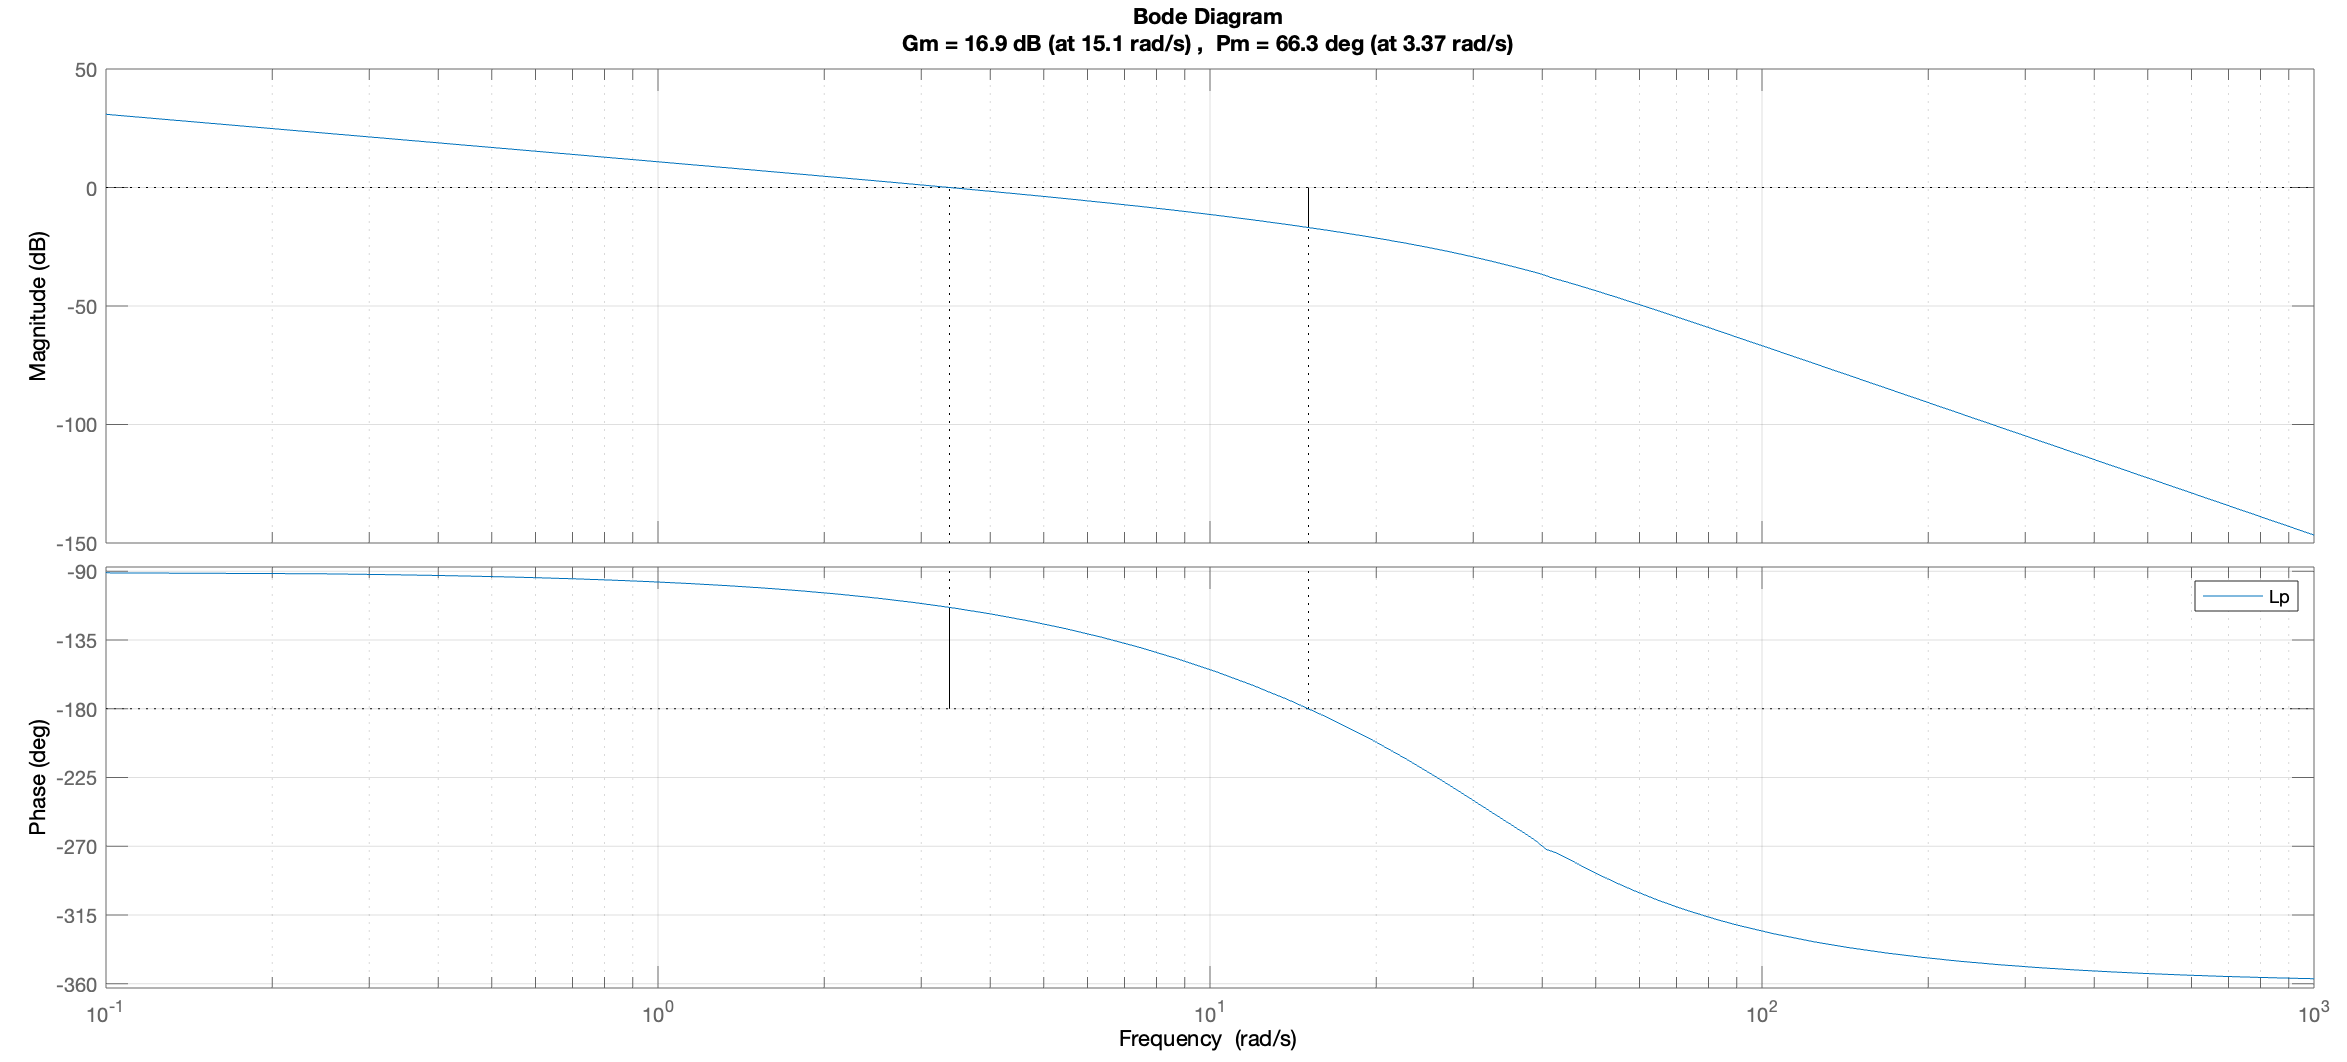
\includegraphics[width=\textwidth]{openloop_margin_pos_1dof}
		\subcaption{Open-loop Bode diagram}
	\end{subfigure}
	\begin{subfigure}{0.45\columnwidth}
		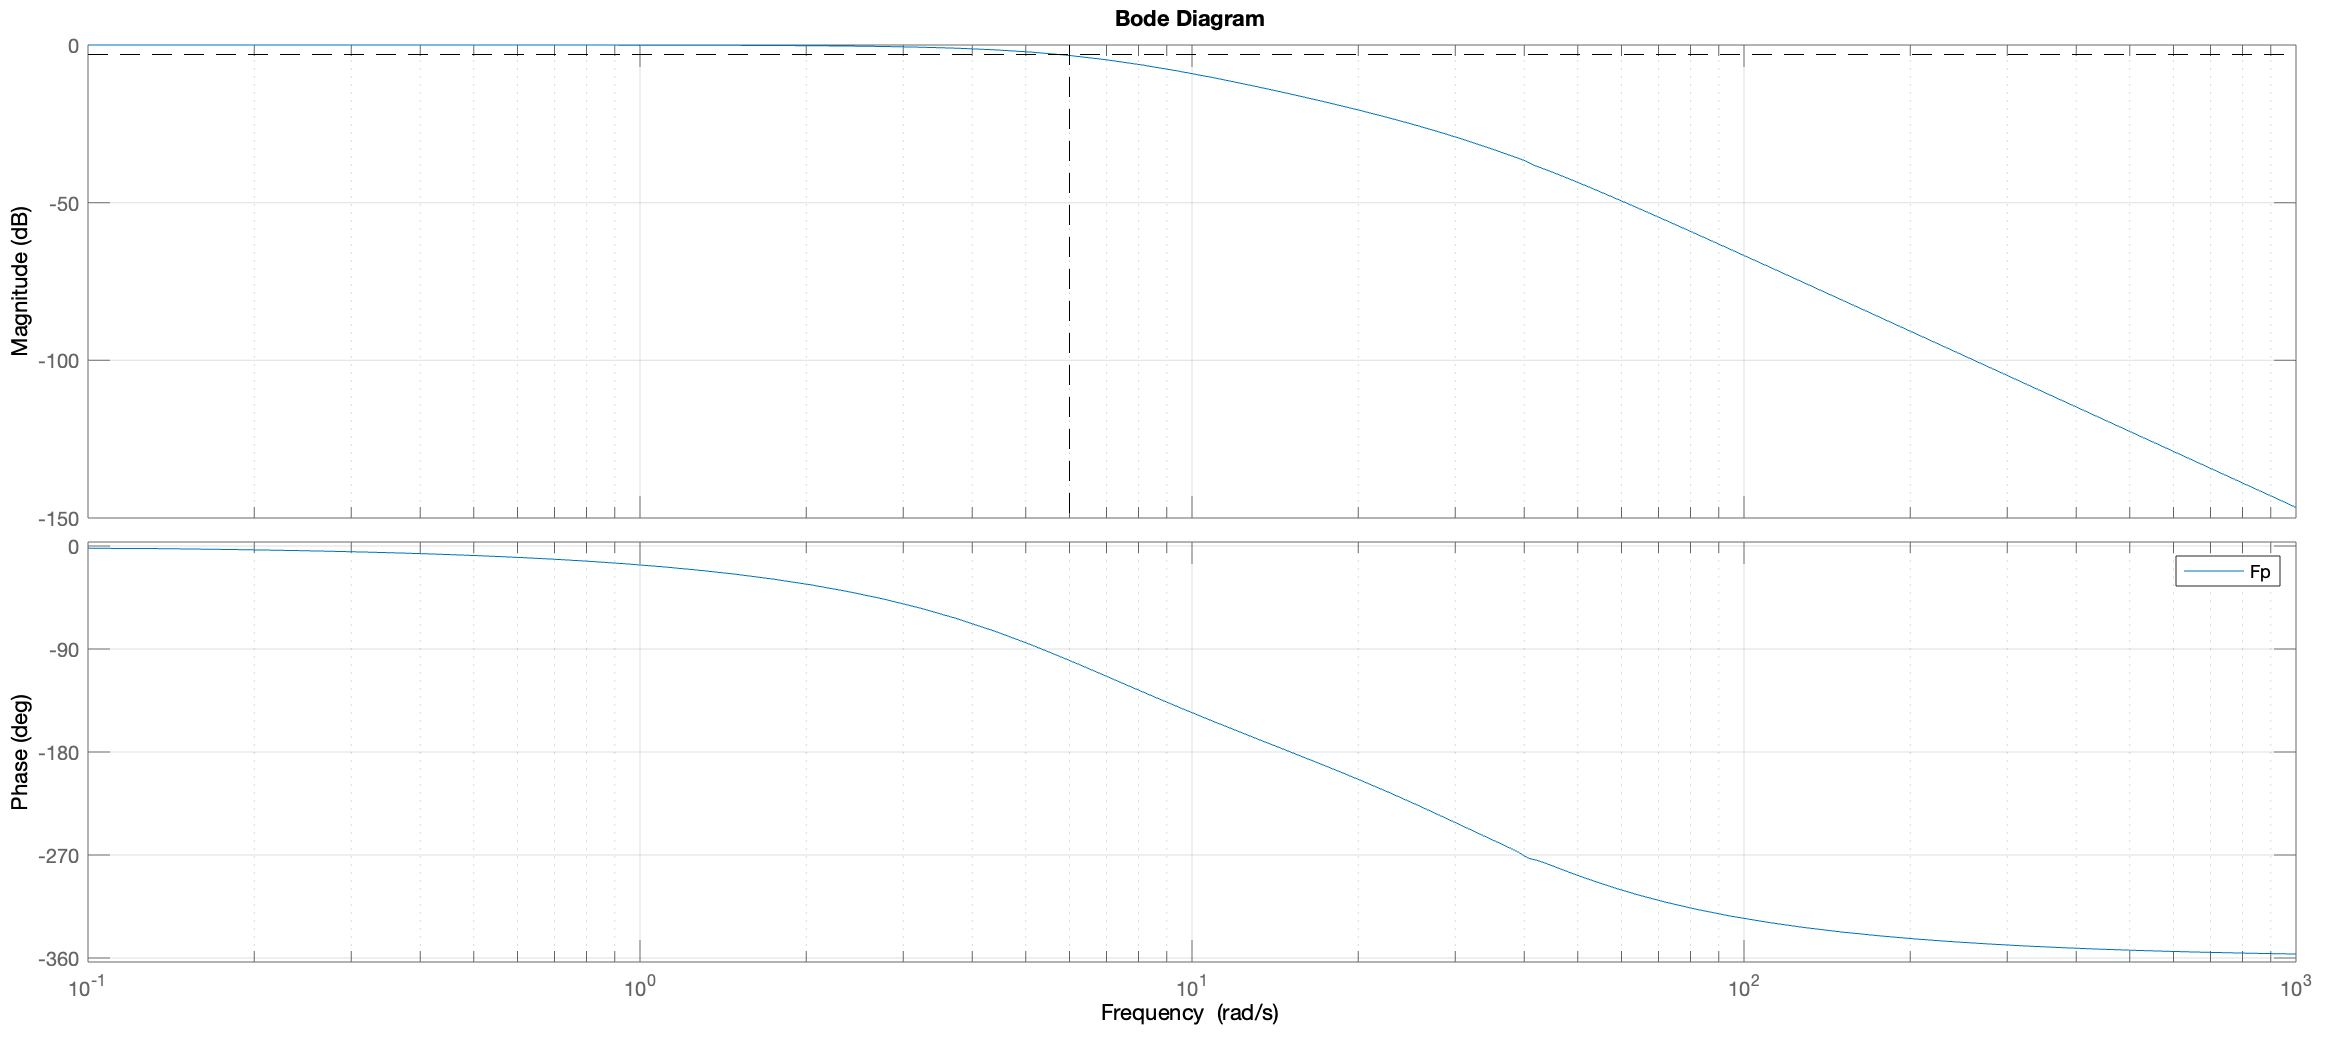
\includegraphics[width=\textwidth]{closedloop_bode_pos_1dof}
		\subcaption{Open-loop Bode diagram}
	\end{subfigure}
	\caption{Bode diagrams with  $k_p=3.5\ rad/s$}
	\label{fig:Bode P 3.5}
\end{figure*}

\paragraph{Performance analysis}
Due to the friction, the position reached by the mass is not exactly the reference one. The controller integrates this small error and the control input raises slowly. Since the static friction coefficient is higher than the dynamic one, the load will move only after a few seconds, during which the controller has kept integrating the error asking for an increasing control action.
Once that the input is large enough to counteract the static friction, the load moves and the friction drops, making the applied control input stronger than what needed. The result is that the load moves over the reference, generating an error that is even bigger than the original one.
For the above-mentioned reasons, a logic switch has been implemented. Its purpose is that of deactivate the integrative action of the inner loop whenever the position error is smaller than a threshold equal to~$0.85 \degree$, that corresponds to 10 pulses of the encoder and is a bit greater than the maximum static error due to friction. On the other hand, it is not possible to zero error at steady state since only the proportional action is in place.
\begin{figure*}
	\centering
	\begin{subfigure}{0.45\columnwidth}
		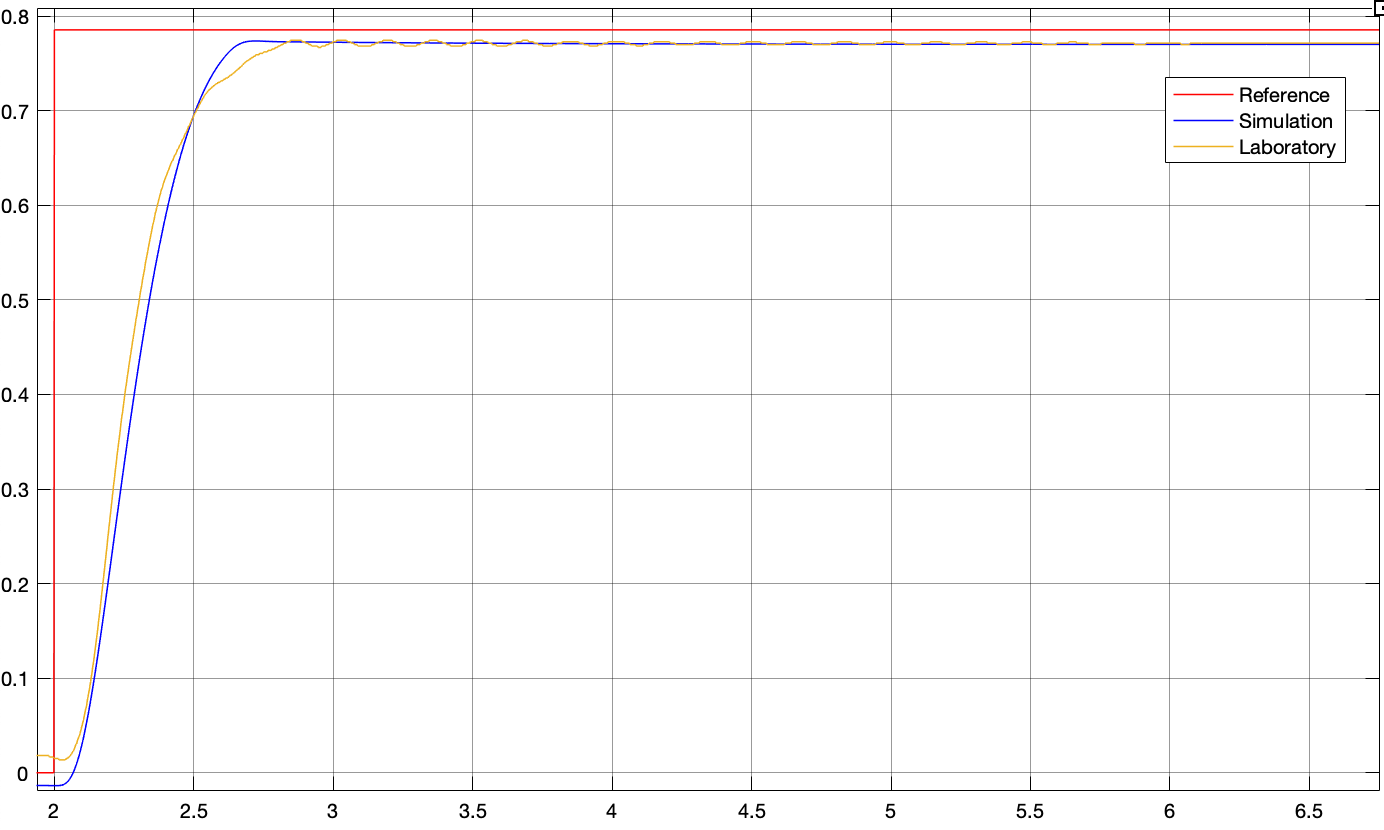
\includegraphics[scale=0.3]{pos_1_dof}
		\caption{Position}
	\end{subfigure}
	\begin{subfigure}{0.45\columnwidth}
		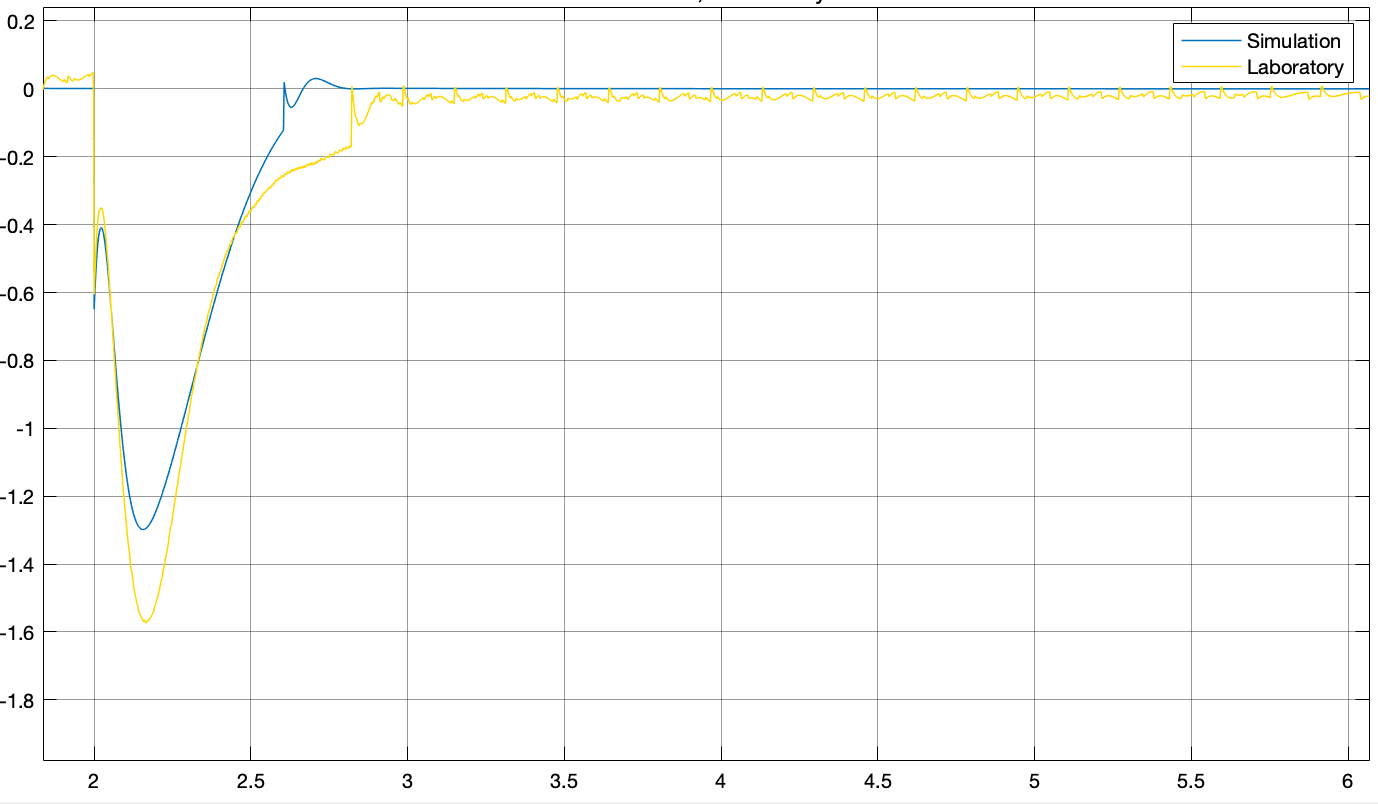
\includegraphics[scale=0.3]{volt_1_dof}
		\caption{Voltage}
	\end{subfigure}
	\caption{Step response with $k_p=3.5$}
	\label{fig:Pos_1dof_3.5}
\end{figure*}

\paragraph{Bandwidth and phase margin estimation}
Also in this case, a sine-sweep experiment is performed to estimate the bandwidth of the closed-loop system. Simulation and laboratory data are really close, as their cutting frequency estimation: the first one is around~$5.6\ rad/s$, the second one~$5.3\ rad/s$.
\begin{figure*}[h]
	\centering
	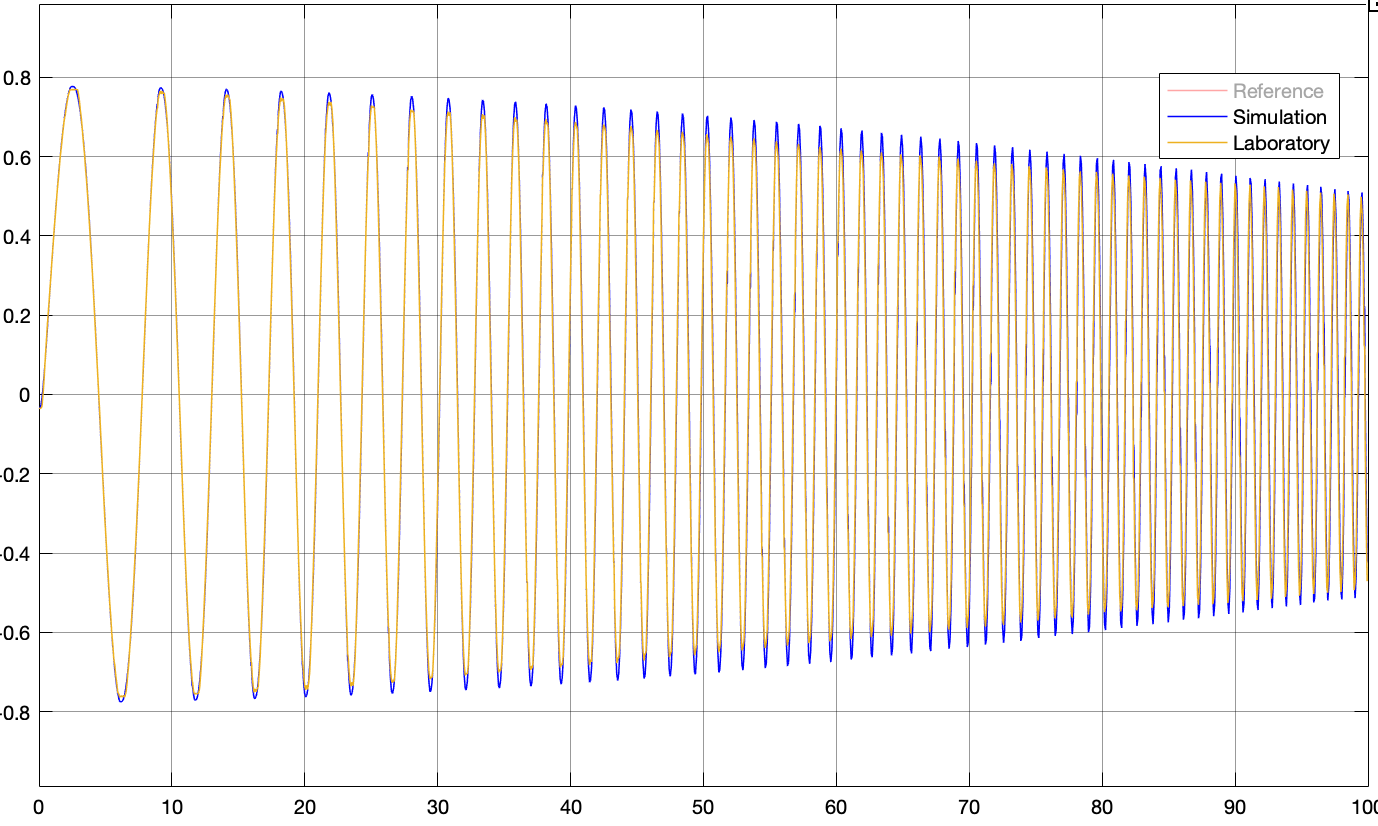
\includegraphics[width=0.9\columnwidth]{sine_pos_1dof}
	\caption{Sine-sweep experiment from $0.1\ Hz$ to $1\ Hz$ in $100\ s$}
	\label{fig:sinesweep_pos_1dof}
\end{figure*}
According to the fact that there are not oscillations and overshoots, it is expected a high phase margin that is supposed to be very close to the theoretical one, reported in the comparison table.

\section{\twodof\ system}
The objective in this case is the same of the previous one: a quite fast control, limiting oscillations as possible. Now, consider the transfer function from voltage to the second mass speed:
\[
G_{v,\dot{\theta}_2}(s)=
\frac{-1.293 \cdot 10^{8}}{s^5+40.9s^{4}+4833s^{3}+1.686 \cdot 10^{5} s^{3}+3.327 \cdot 10^{6} s+7.355 \cdot 10^{7}}
\]
\begin{figure*}[h]
	\centering
	\begin{subfigure}{0.4\columnwidth}
		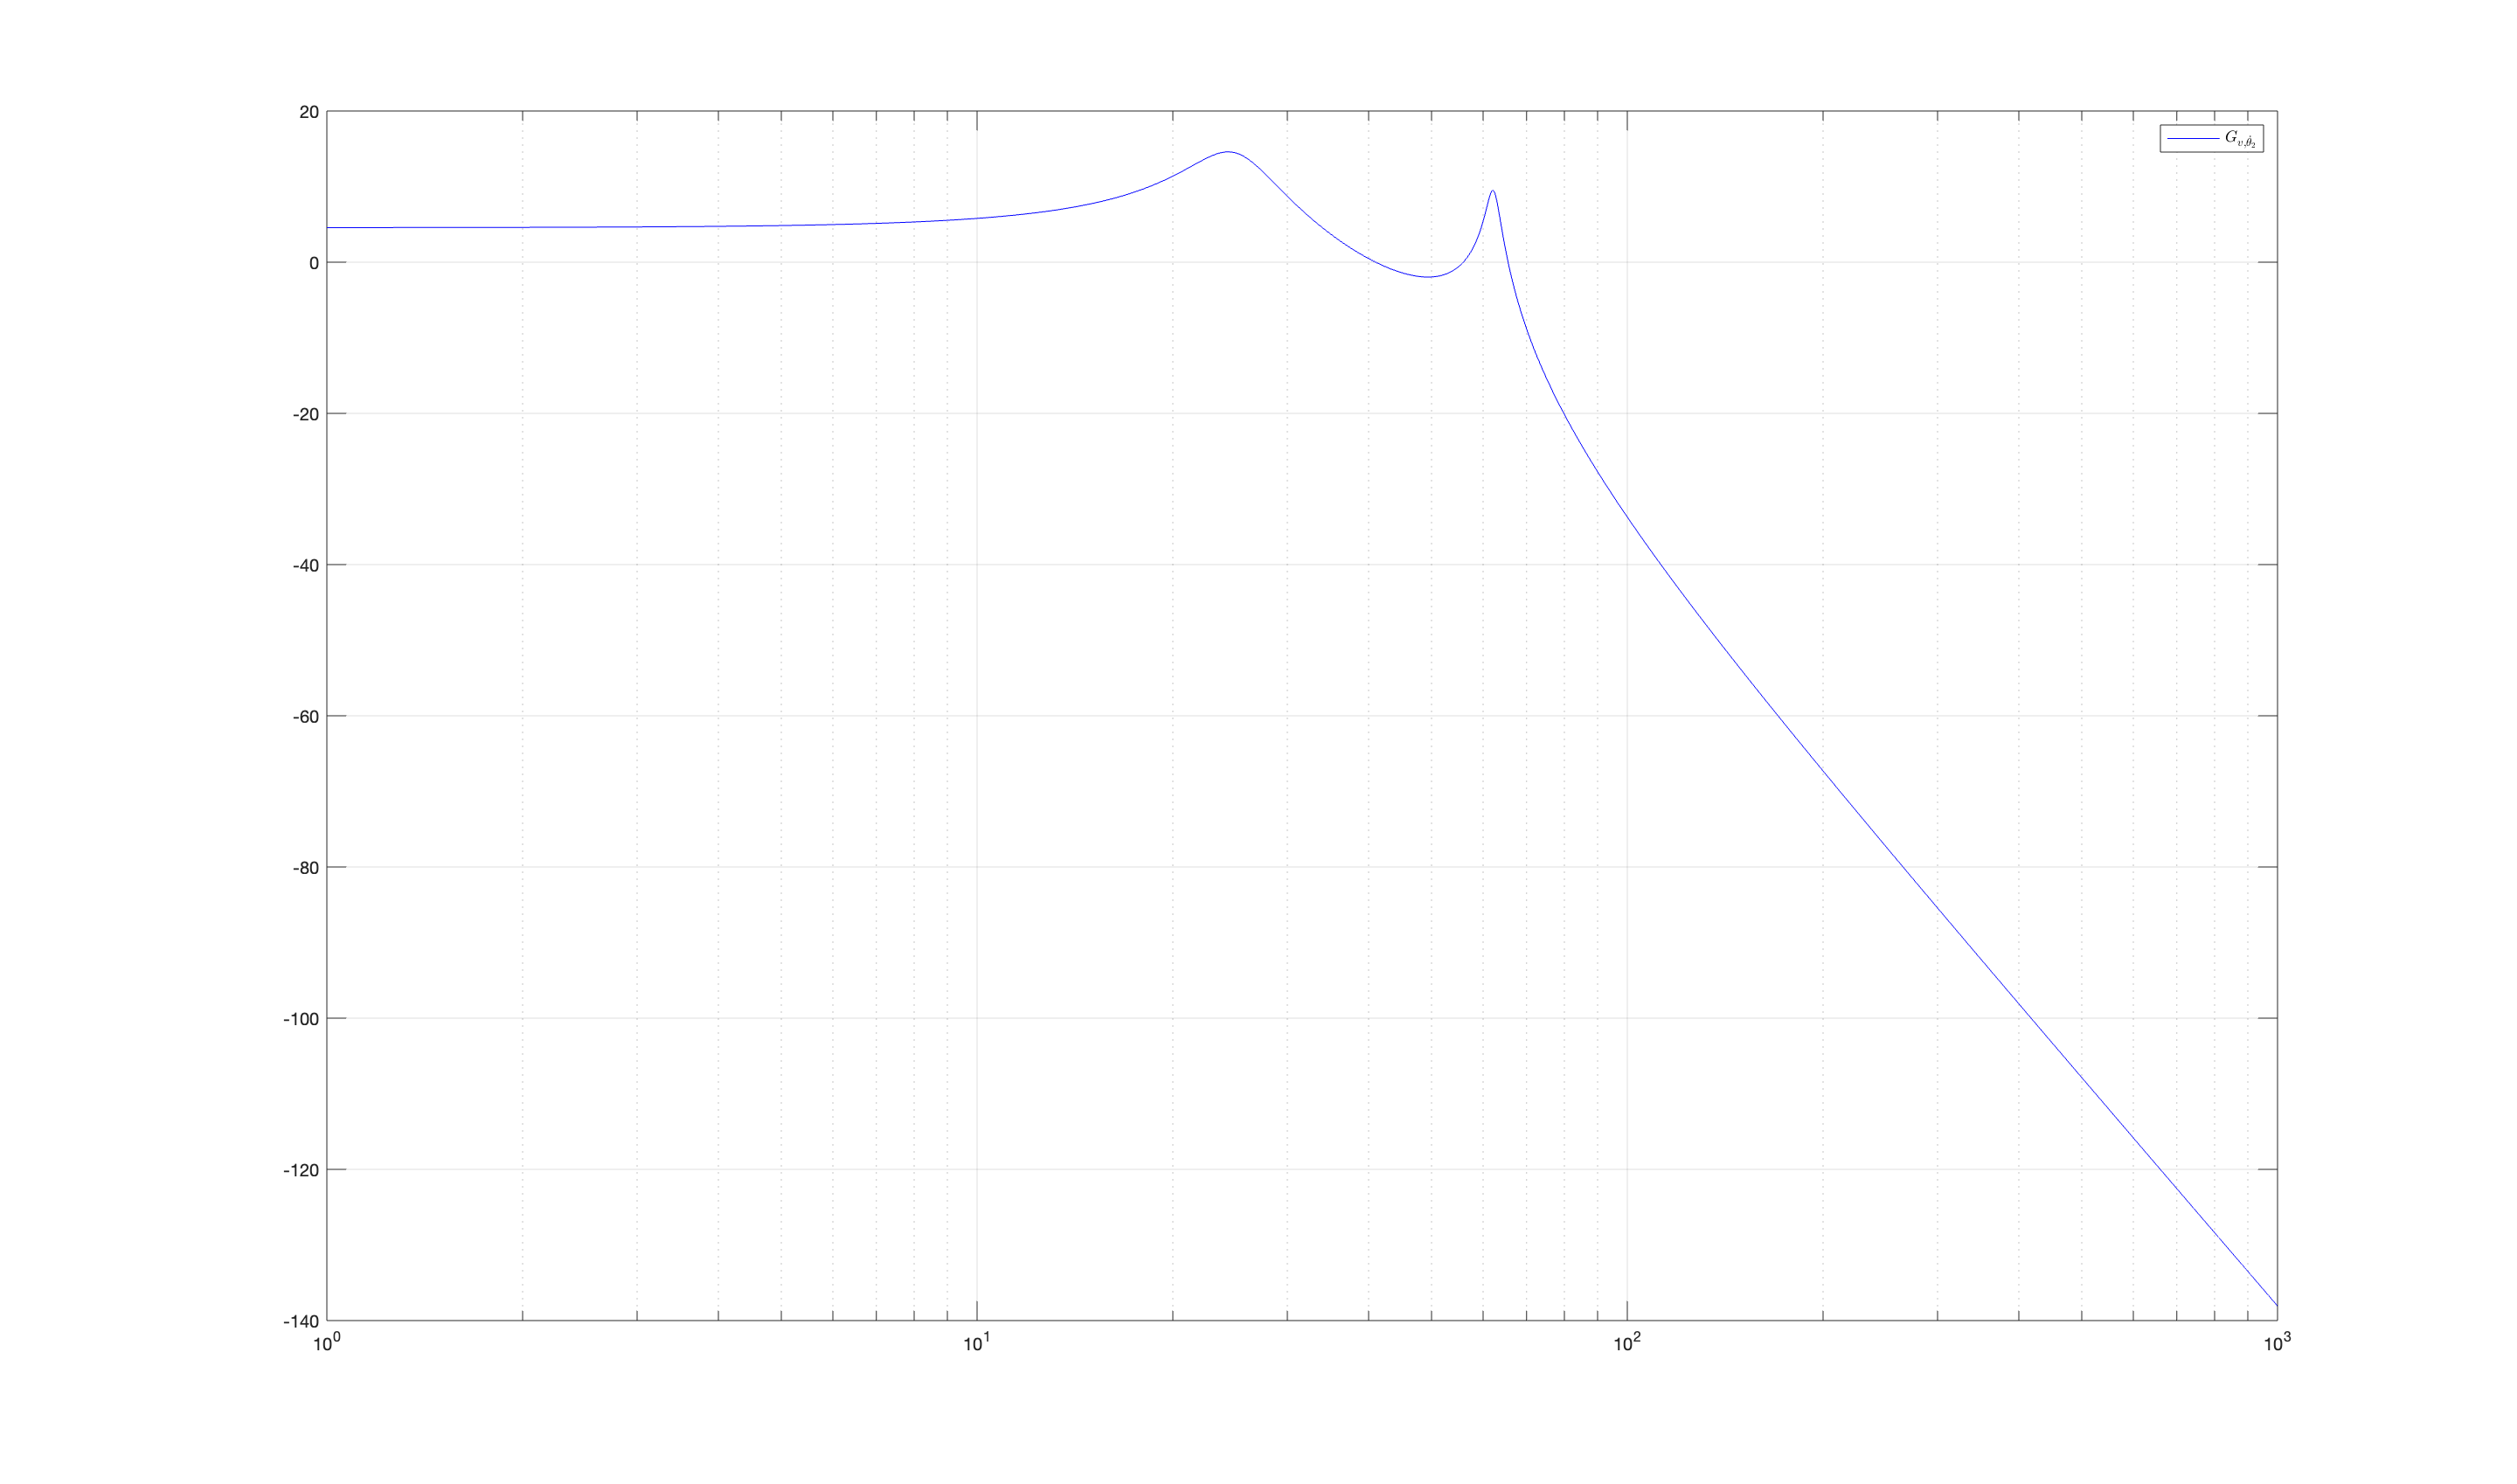
\includegraphics[width=\textwidth]{1_bodeG2}
	\end{subfigure}
	\begin{subfigure}{0.4\columnwidth}
		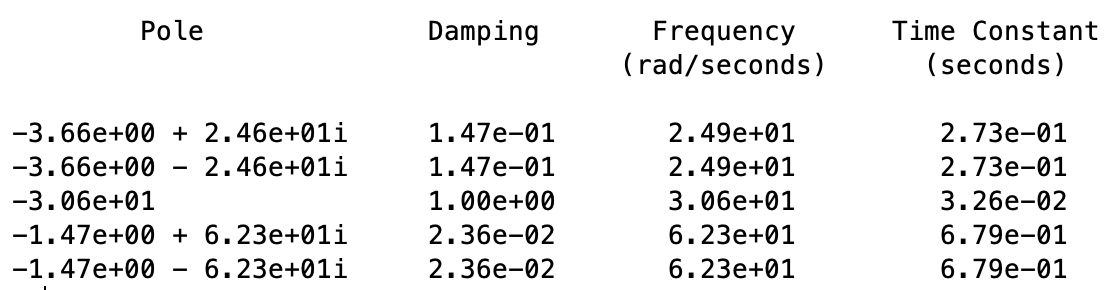
\includegraphics[width=\textwidth]{1_poleG2}
	\end{subfigure}
	\caption{G(s)}
	\label{fig:G(s)2dof}
\end{figure*}

As it is possible to notice in \cref{fig:G(s)2dof}, there are now two couples of complex conjugated poles with low damping coefficient. A similar solution to the \onedof\ problem has been applied, it is used a notch filter to delete these poles and substitute them with a couple of complex conjugated poles, this time at frequency~$100\ rad/s$ and a damping coefficient equal to~$0.72$. The reason why it has been decided to move ahead the poles frequency instead of using the original one is explain in the speed control loop section.
\begin{figure*}[h]
	\centering
	\begin{subfigure}{0.45\columnwidth}
		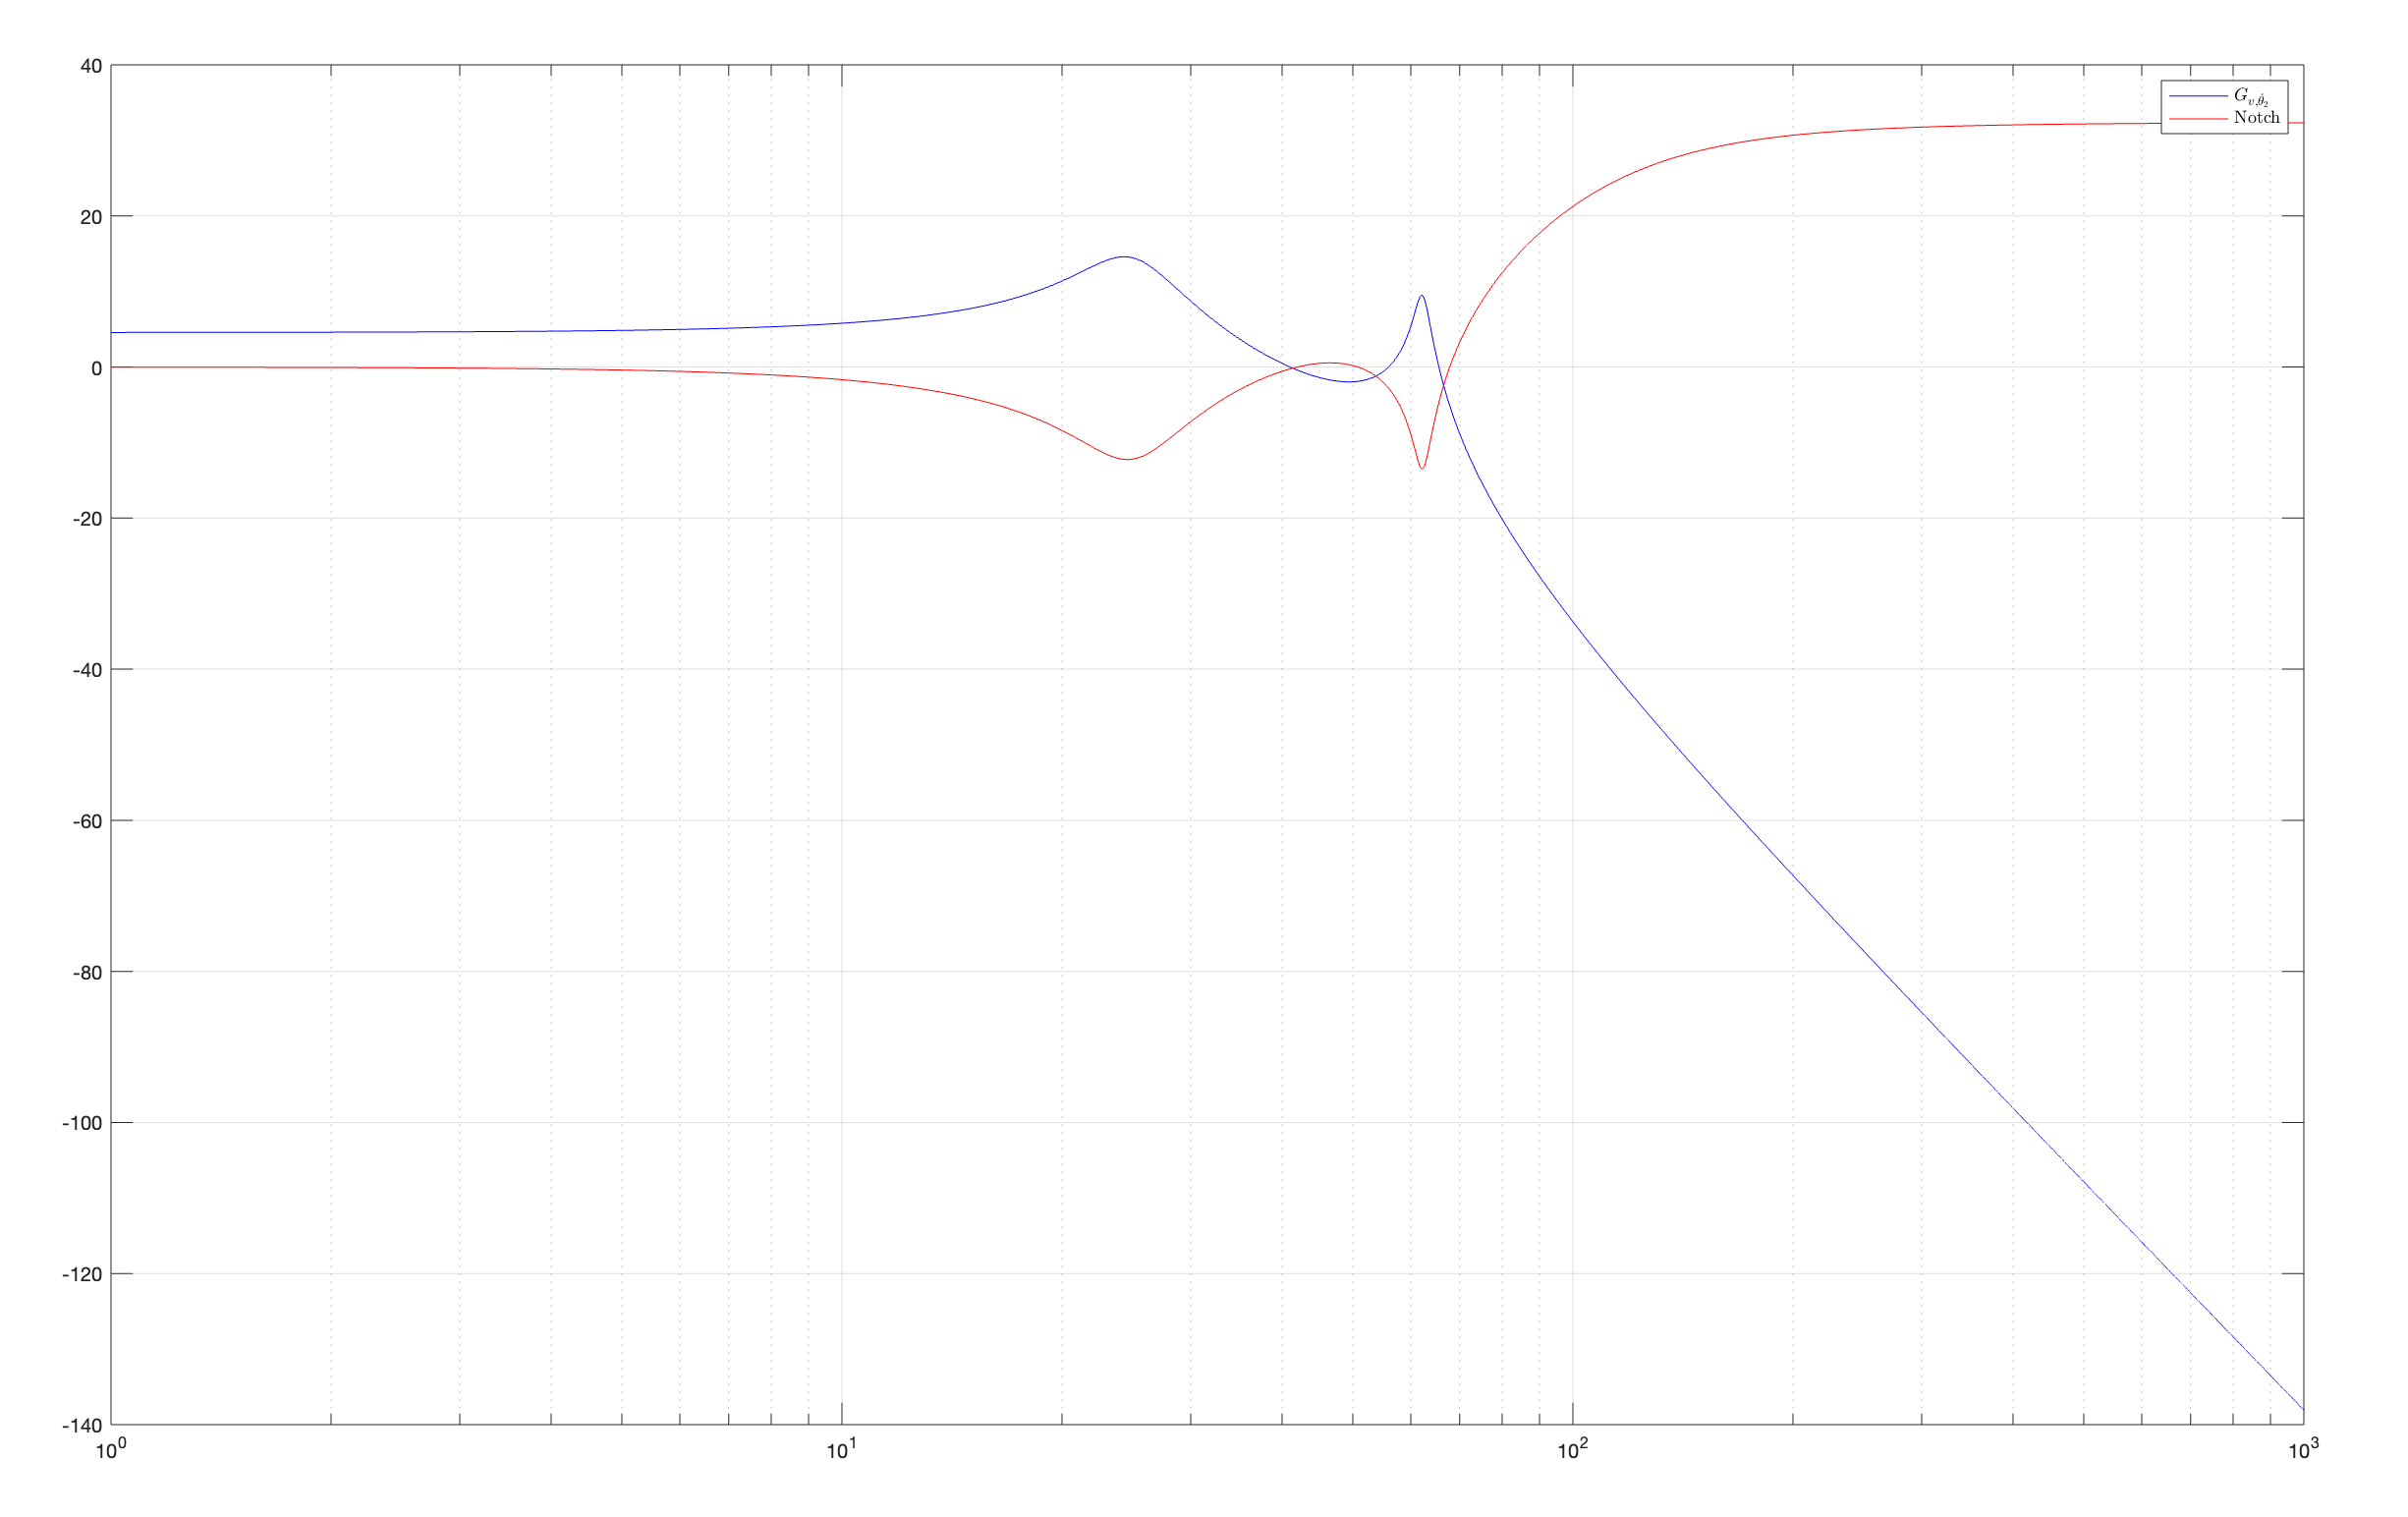
\includegraphics[width=\textwidth]{1Nf_G2}
		\subcaption{$N_f(s)$ and $G(s)$}
		\label{fig:Notch Filter2}
	\end{subfigure}
	\begin{subfigure}{0.45\columnwidth}
		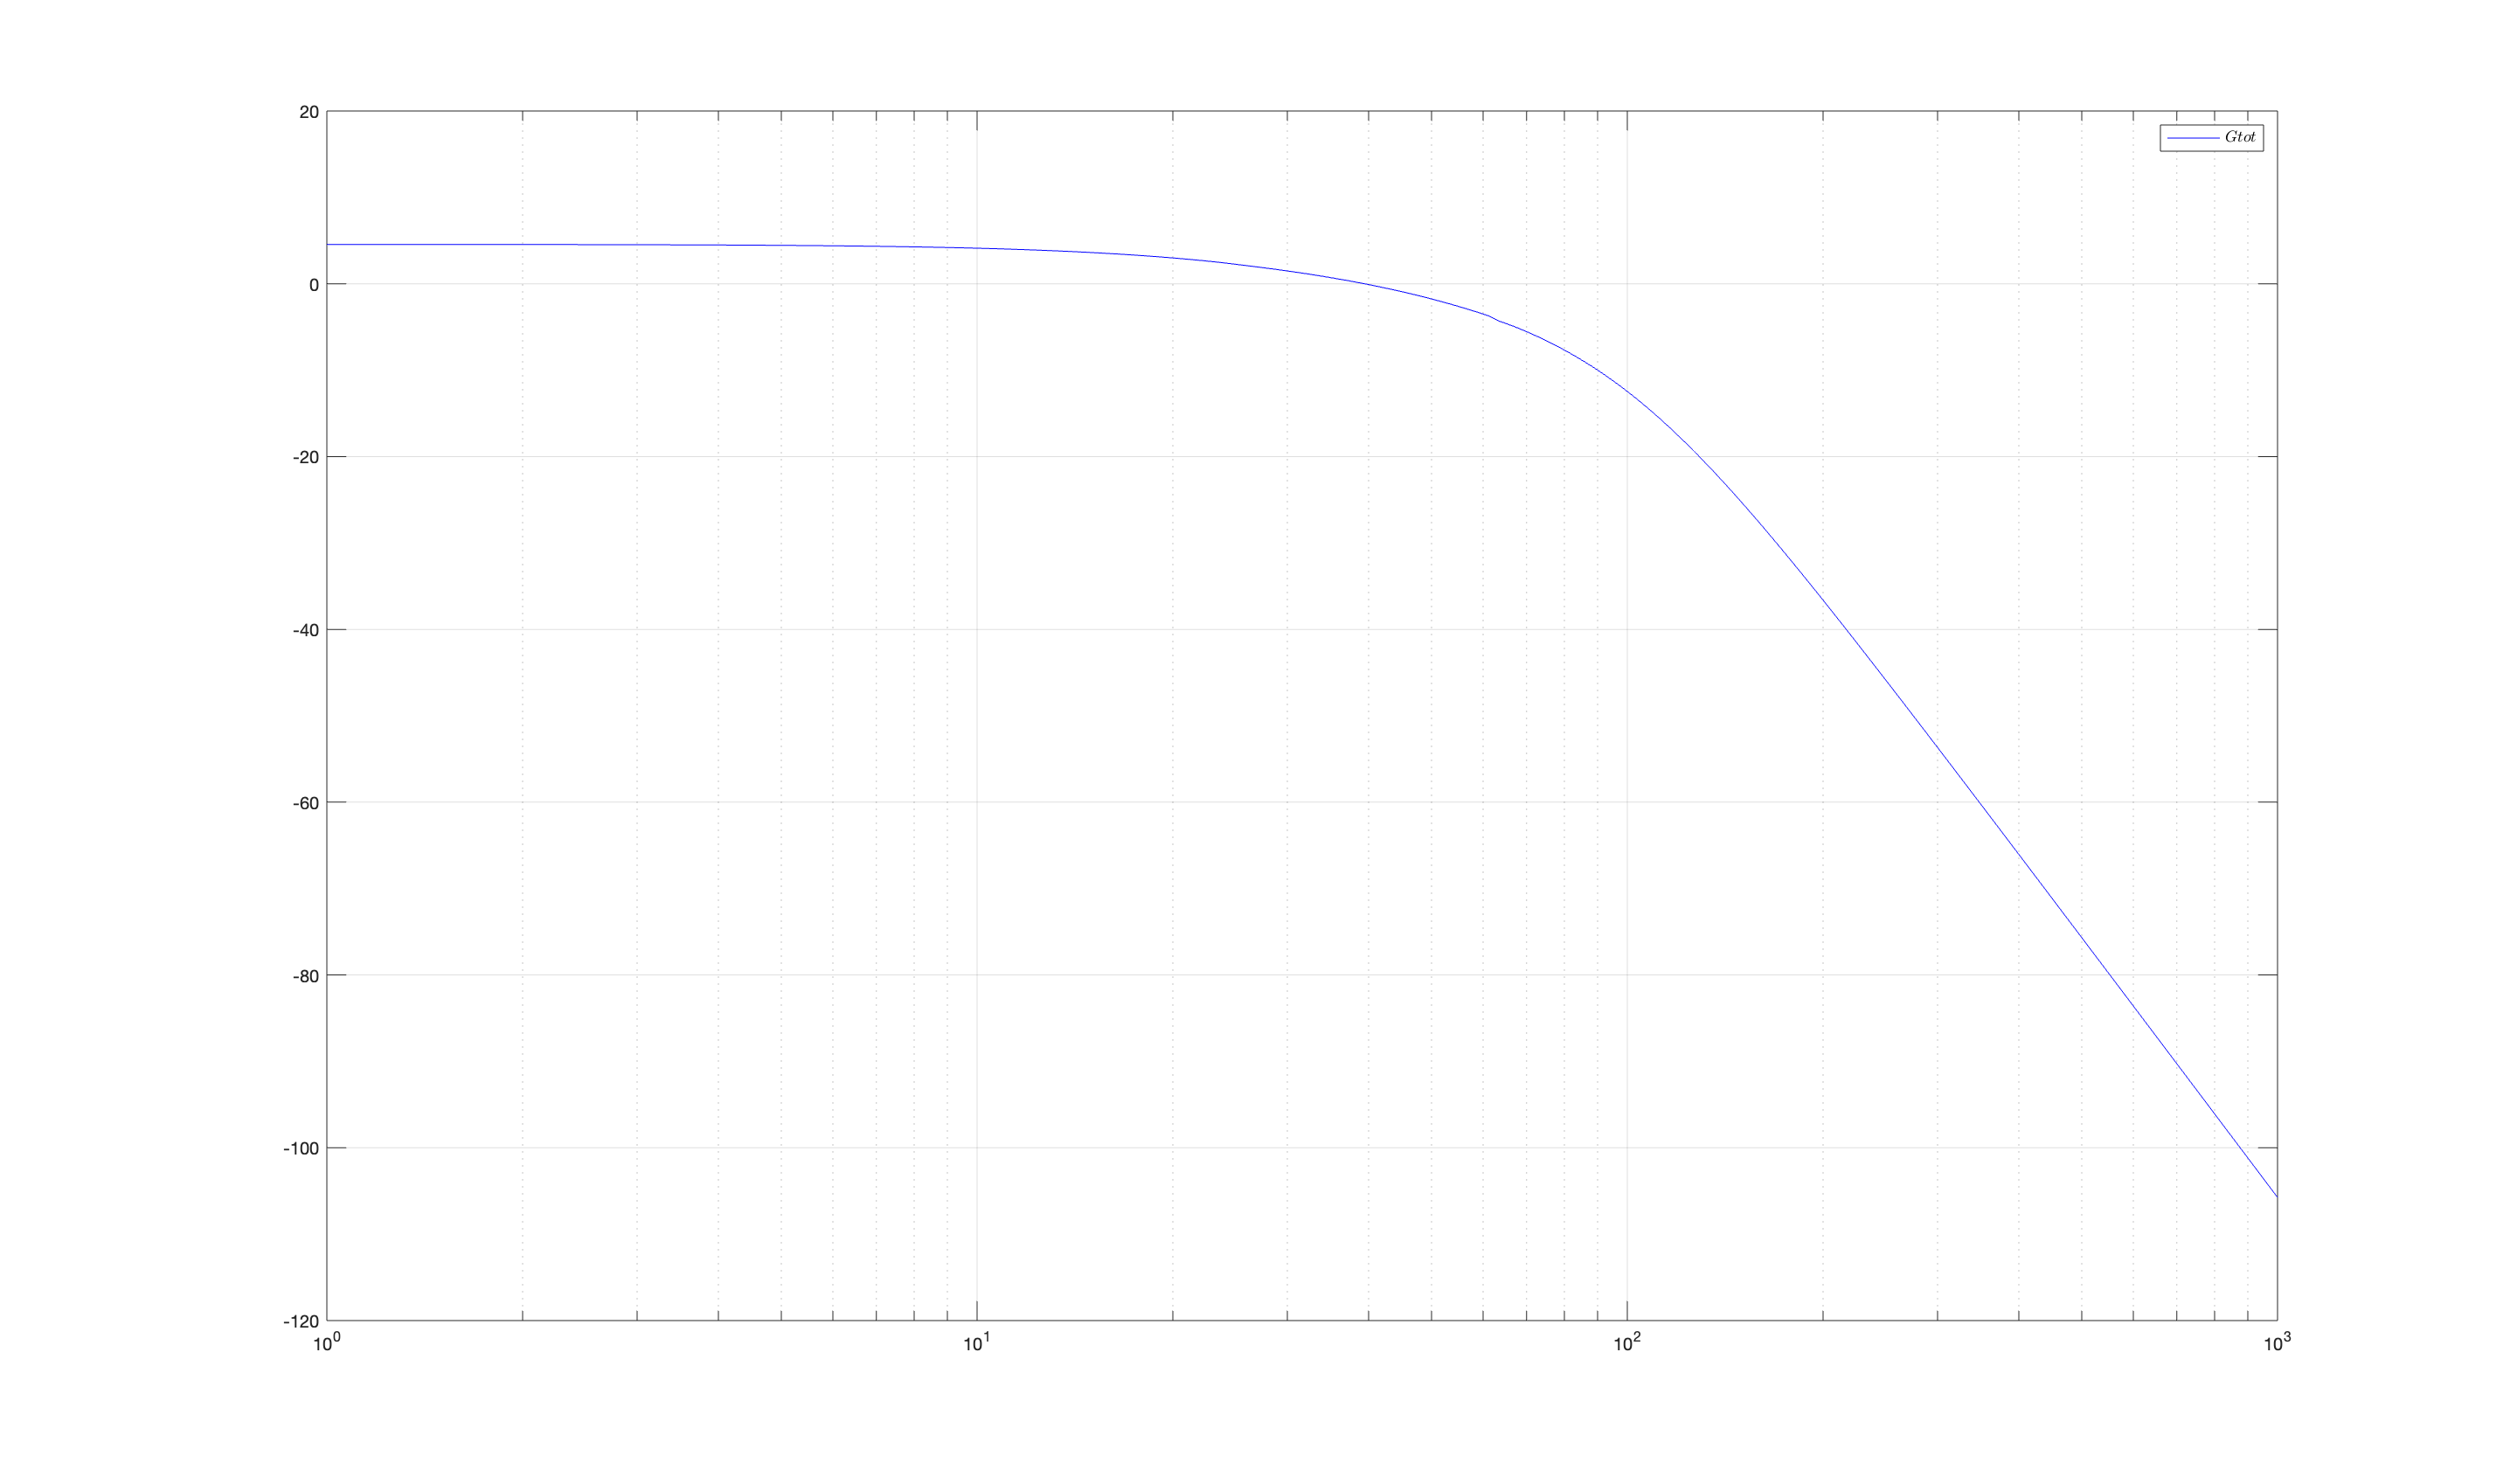
\includegraphics[width=\textwidth]{1_G2tot}
		\subcaption{$G_{tot}(s)$}
		\label{fig:Plant G(s) with Notch Filter2}
	\end{subfigure}
	\caption{Plant $G(s)$ with Notch Filter $N_f(s)$: $G_{tot}$(s)}
\end{figure*}

Applying the notch filter represented in \cref{fig:Notch Filter2}, the controller sees the plant~$G_{tot}(s)$ of \cref{fig:Plant G(s) with Notch Filter2}.

\subsection{Speed Control Loop}
The controller structure is the PI, enriched with an anti-windup; as before, the zero of the PI controller cancels out the real pole at~$30.6\ rad/s$.
\[
R(s)=-k_v
\frac{\frac{s}{30.6}+1}{s}
\]
\begin{figure*}[h]
	\centering
	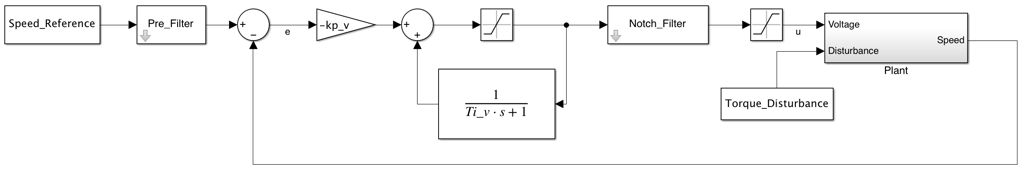
\includegraphics[width=0.8\textwidth]{2dof_PI_scheme}
	\caption{Closed-loop block scheme}
\end{figure*}

\paragraph{Tuning and simulation}
As noticed in the \onedof~case, there are some periodic oscillations due to a change of the dynamic friction along the revolution of the masses. 
Right now, the amplitude of these disturbances cannot be neglected anymore and a solution to attenuate them as much as possible needs to be found. In order to enhance the disturbance rejection, a~$w_{c,v}$ high enough to obtain a large bandwidth is required. On the other hand, it is not possible to set it at too high frequencies, otherwise the phase margin would decrease dramatically. In order to design the right controller, in the simulation scheme of~$G(s)$ it has been added a disturbance: it acts as a torque on (\textit{mass1} and \textit{mass2}) shafts, with fixed amplitude at~$0.005\ Nm$ and frequency equal to the masses speed, to simulate the dynamical change of friction during the revolution. \\
A first possible tuning is the following:
\begin{figure*}[h]
	\centering
	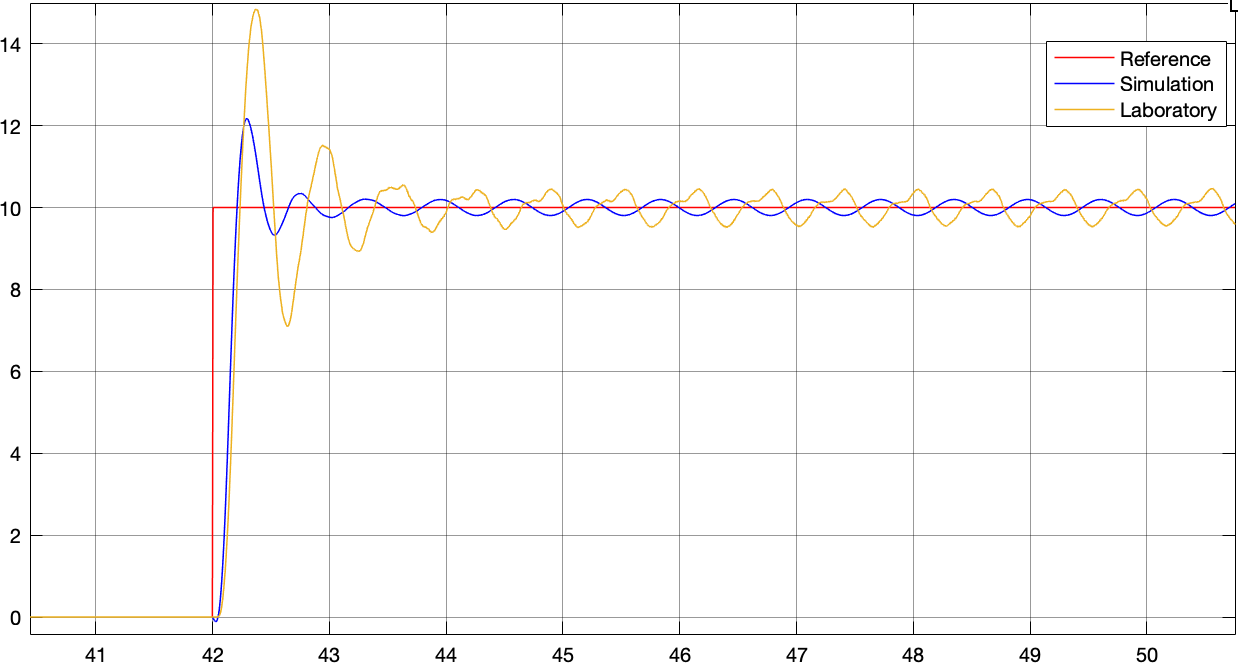
\includegraphics[scale=0.4]{step10_noPF}
	\caption{Step response with $k_v=5$}
	\label{fig:step10_noPF}
\end{figure*}
\\
This solution is far to be acceptable, due to its high oscillations during the transient. To keep large enough the bandwidth, it has been decided not to anticipate the~$w_{c,v}$, but to build a low-pass pre-filter on the reference signal. Thanks to this solution, the closed-loop system will not be excited by high frequencies; moreover, even the uncertainty on resonances do not produce differences between simulation and experiments at the laboratory.
Many settings have been tried: in \cref{fig:2dof_PI_trials} is shown the comparison between these two configurations. The \textit{tuning 2}, starting from the previous experiment (\cref{fig:step10_noPF}), cancels out the transient oscillations by means of the low-pass pre-filter; then, the \textit{tuning 1} tries to enlarge the bandwidth even more.
\begin{figure*}[h]
	\centering
	\begin{subfigure}{0.45\columnwidth}
		\centering
		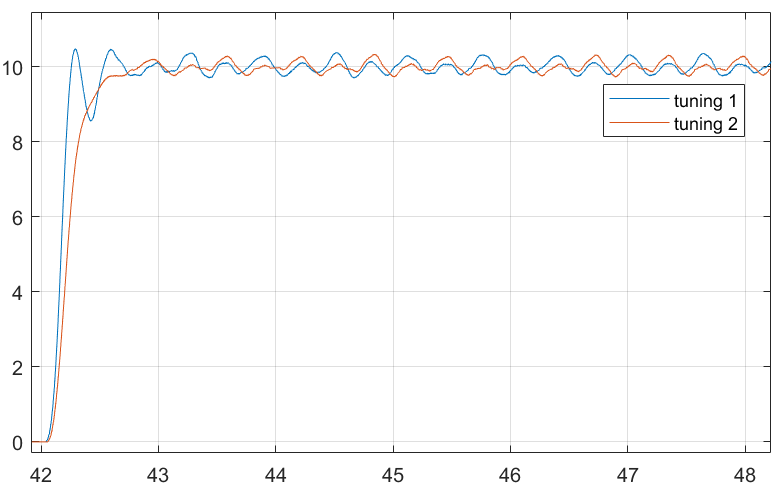
\includegraphics[width=0.8\textwidth]{2dof_PI_trials}
		\subcaption{Closed-loop step responses}
	\end{subfigure}
	\begin{subfigure}{0.45\columnwidth}
		\centering
		\begin{tabular}{|c|cc|}
			\hline
			& Tuning 1 & Tuning 2 \\
			\hline
			$k_v$ & 10 & 5 \\
			$P_f$ & $\frac{8}{s+8}$ & $\frac{7}{s+7}$ \\
			\hline
		\end{tabular}
		\subcaption{Configuration parameters}
	\end{subfigure}
	\caption{Comparison between two different tunings}
	\label{fig:2dof_PI_trials}
\end{figure*}
In both cases, the settling time is around $0.8\ s$. However, in the first tuning, oscillations in the transient are not considered acceptable because of the too aggressive control action and, therefore, the too low phase margin. Simultaneously, no further disturbance rejection is obtained; hence, our choice is the second tuning.

\paragraph{Performance analysis}
As it is possible to notice in figure \ref{fig:PI_with_5}, the simulation and laboratory data are really close during the transient and the voltage never saturates.
\subparagraph{Oscillations} This solution satisfies the requirements: no oscillations in transient happen and reduction of disturbances amplitude at steady-state. In particular, open-loop disturbances have an amplitude of about~$3\%$ both at~$10\ rad/s$ and~$17\ rad/s$, respectively reduced to~$2.5\%$ and~$1.2\%$ in closed-loop.
\begin{figure*}[h]
	\centering
	\begin{subfigure}{0.4\columnwidth}
		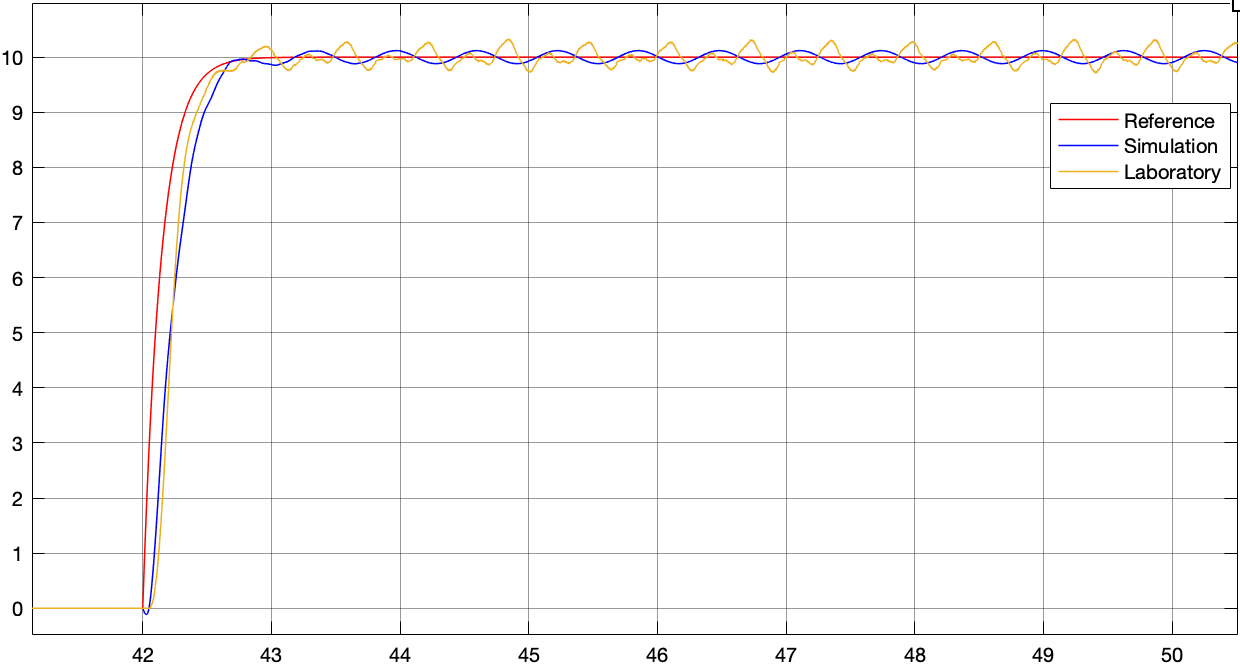
\includegraphics[width=\textwidth]{step10}
		\subcaption{Step of $10\ rad/s$}
	\end{subfigure}
	\begin{subfigure}{0.4\columnwidth}
		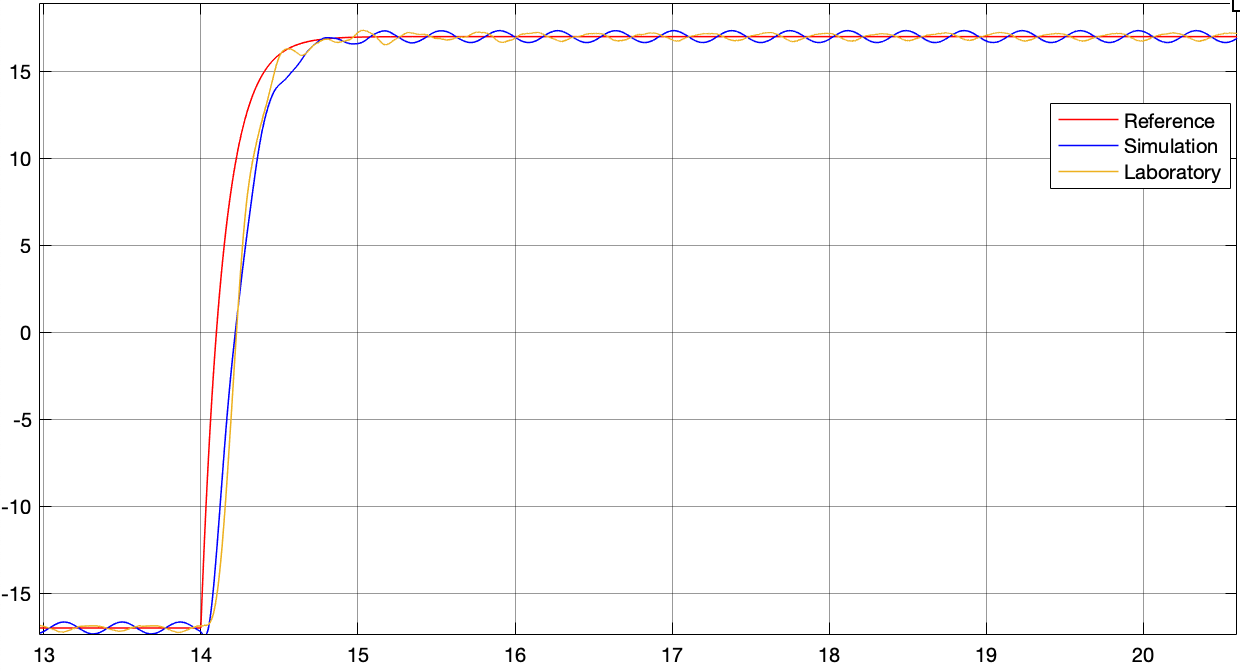
\includegraphics[width=\textwidth]{step17}
		\subcaption{Step of $34\ rad/s$}
	\end{subfigure}
	\begin{subfigure}{0.4\columnwidth}
		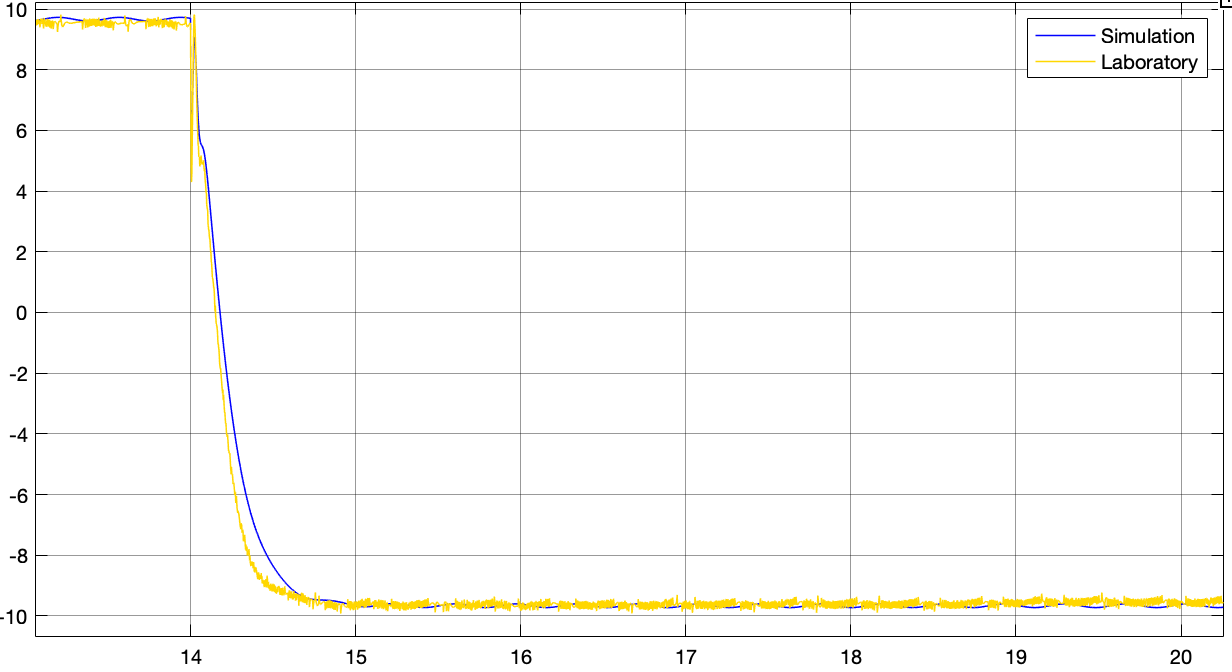
\includegraphics[width=\textwidth]{volt17}
		\subcaption{Voltage related to a step of $34\ rad/s$}
	\end{subfigure}
	\caption{Speed control loop with $k_v=5$ with low-pass pre-filter}
	\label{fig:PI_with_5}
\end{figure*}

\paragraph{Bandwidth and phase margin estimation}
The \cref{fig:sinesweep_speed_2dof} shows the response to a sine-sweep, without applying the pre-filter to the reference. This is useful to estimate the bandwidth of the closed-loop.
\begin{figure*}[h]
	\centering
	\begin{subfigure}{0.45\columnwidth}
		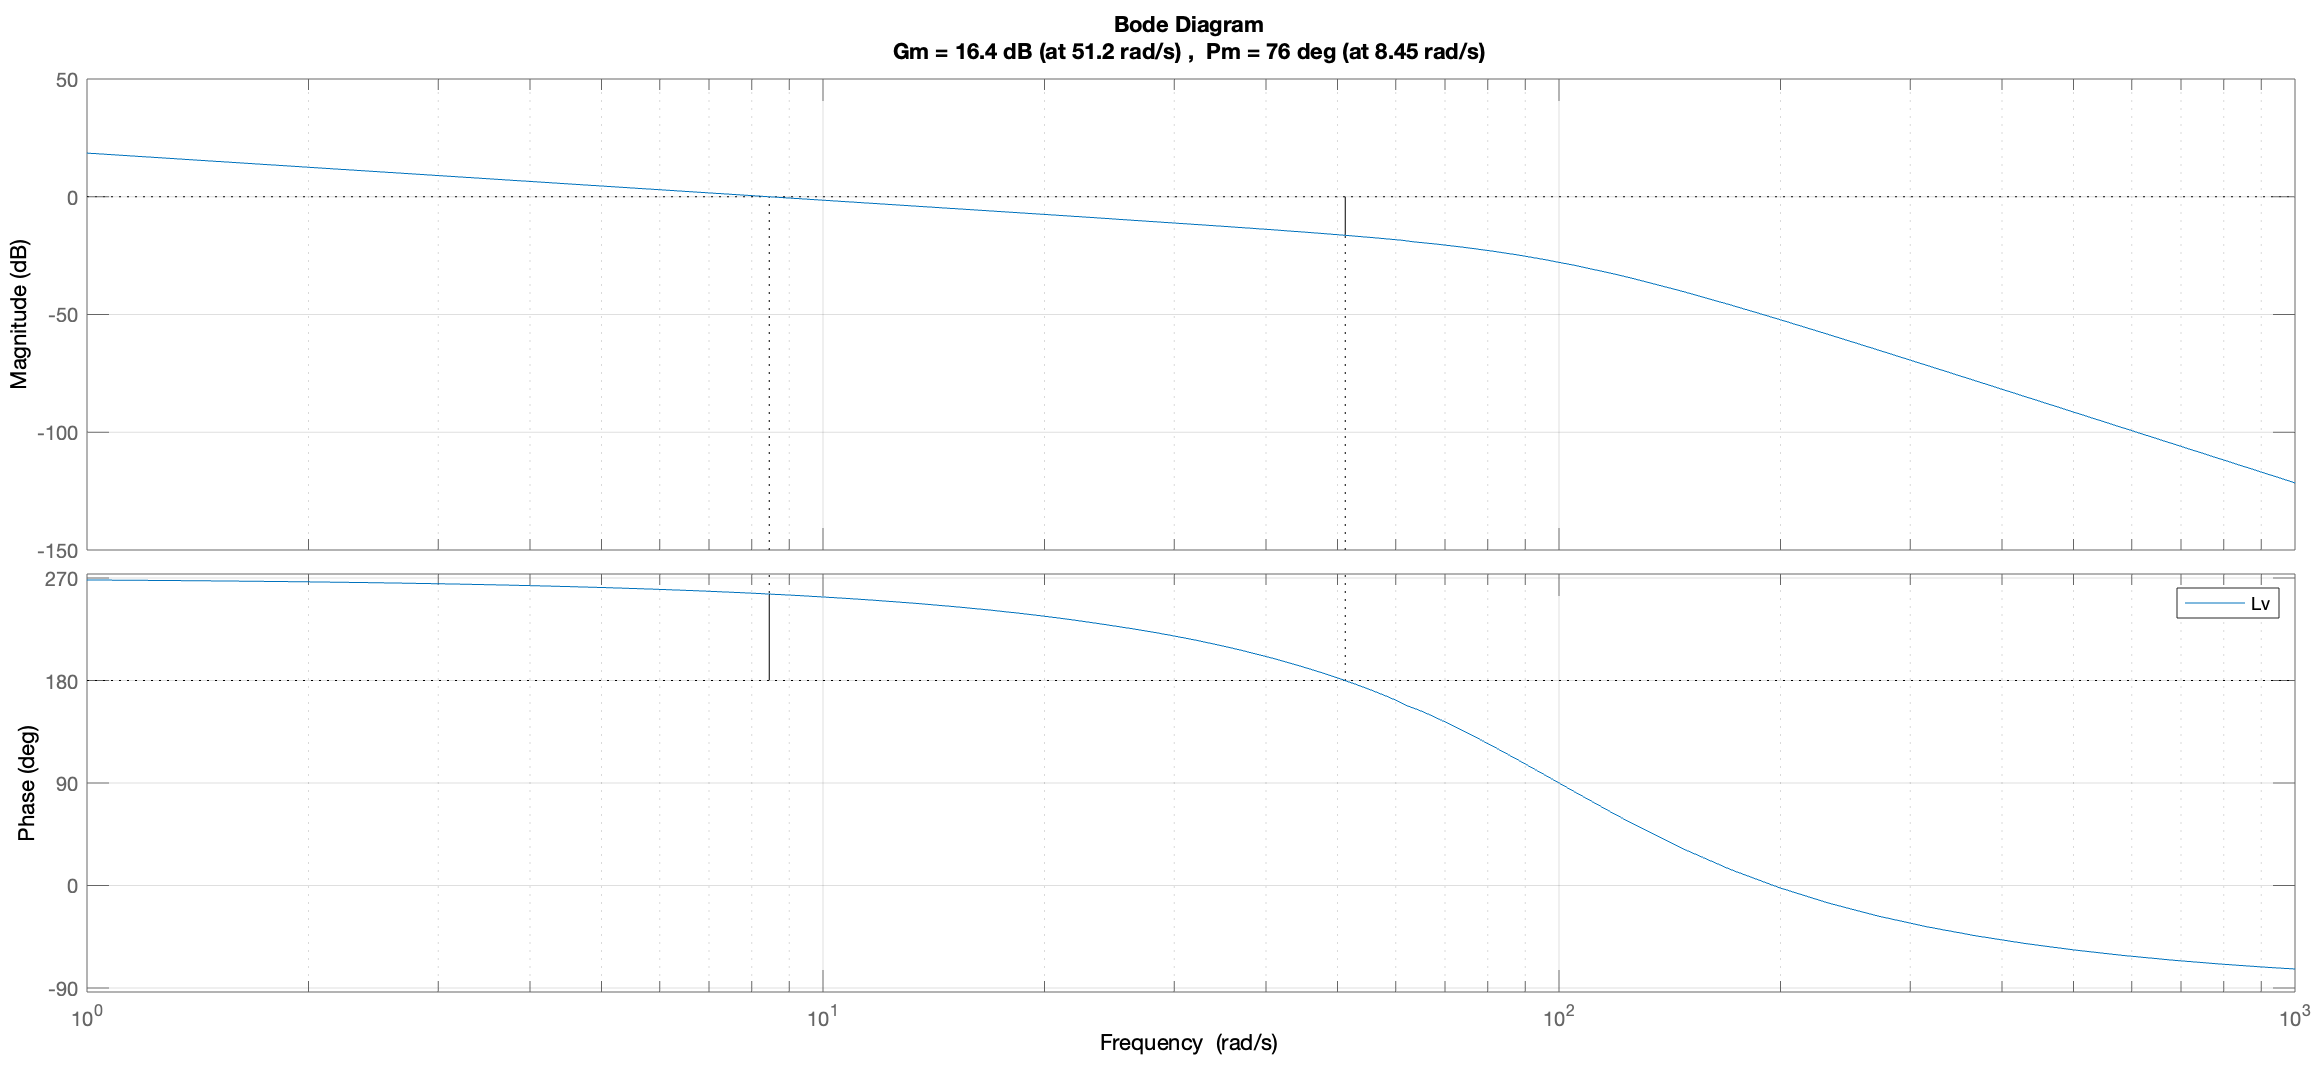
\includegraphics[width=\textwidth]{openloop_margin_speed_2dof}
		\subcaption{Open-loop Bode diagram}
	\end{subfigure}
	\begin{subfigure}{0.45\columnwidth}
		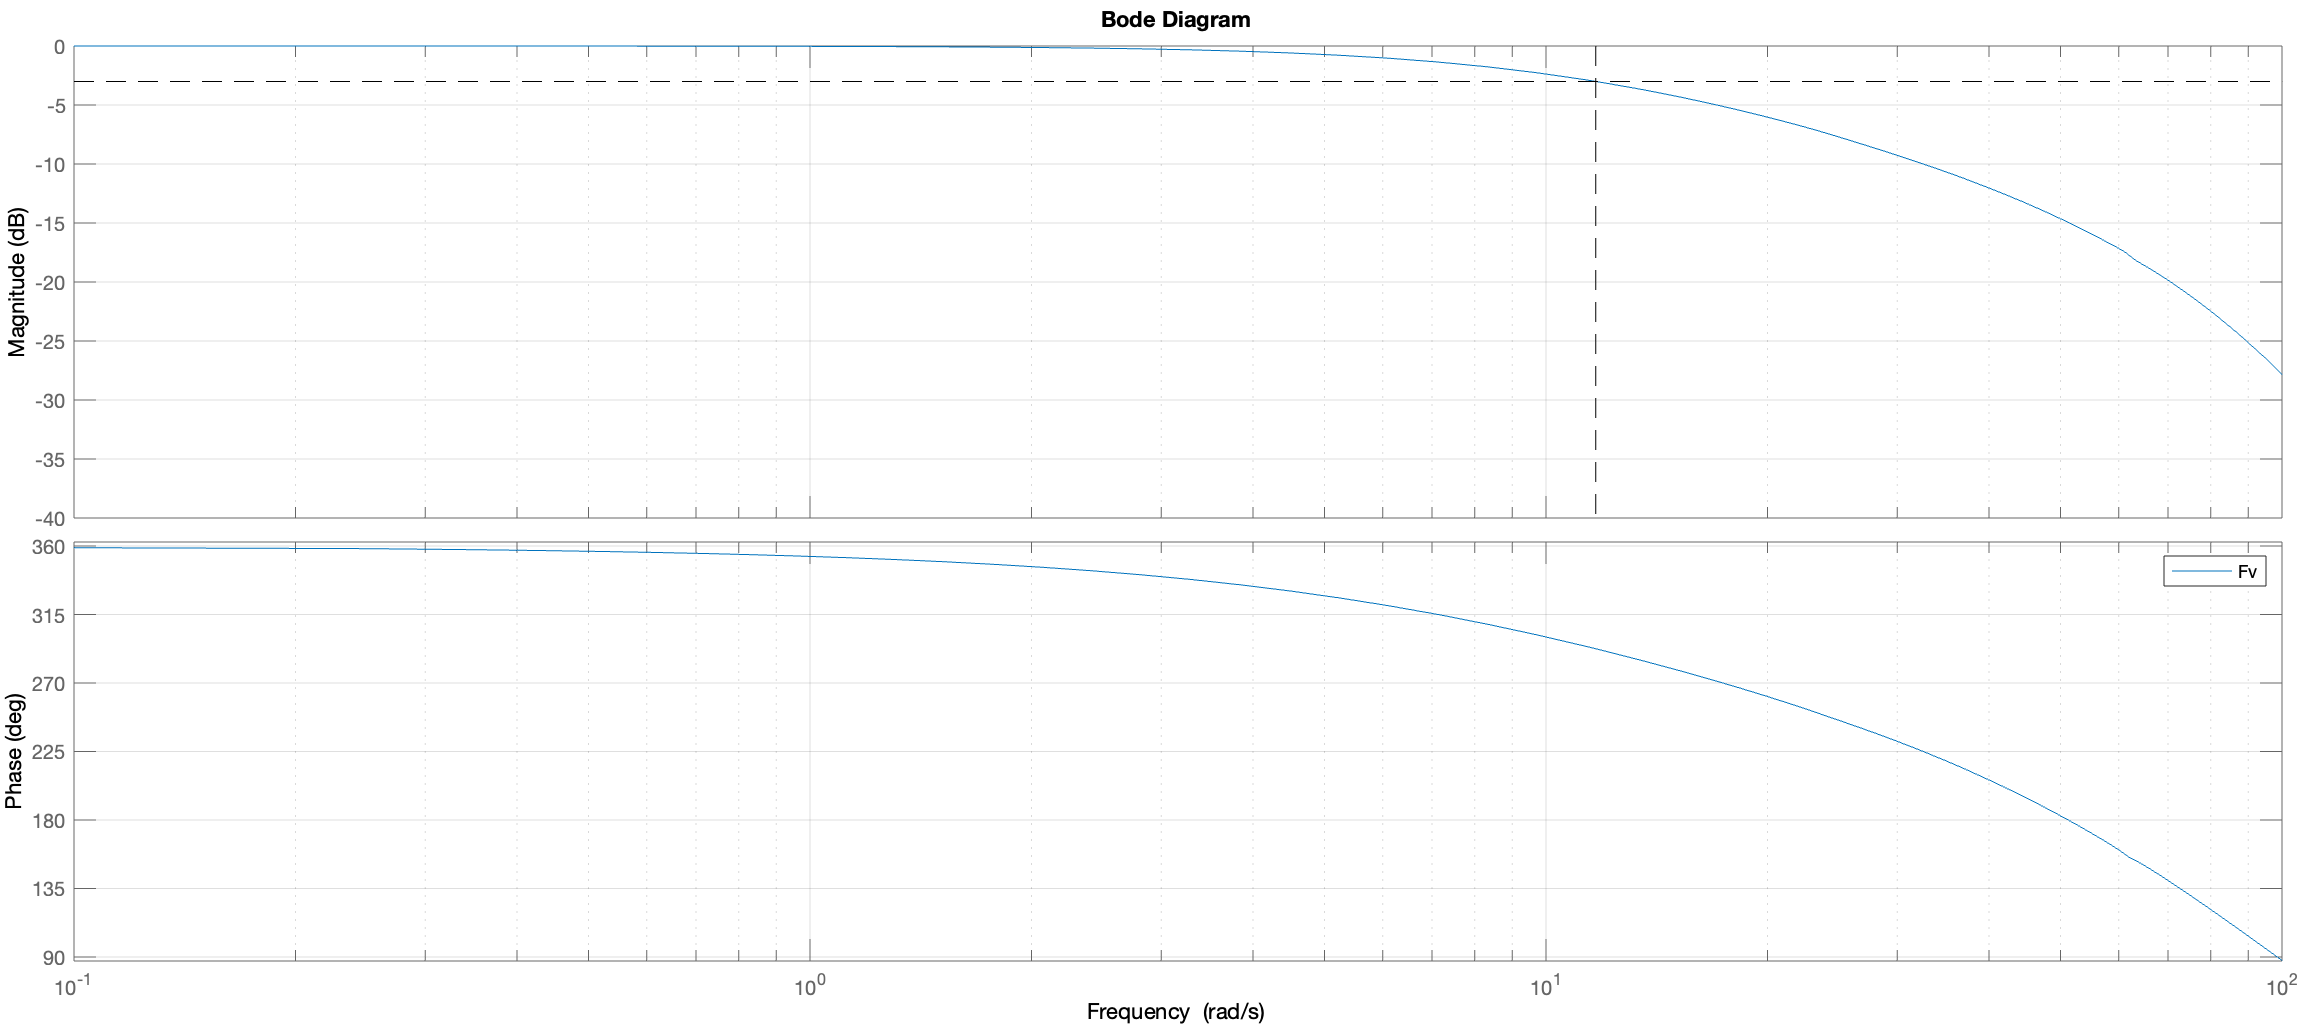
\includegraphics[width=\textwidth]{closedloop_bode_speed_2dof}
		\subcaption{Closed-loop Bode diagram}
	\end{subfigure}
\end{figure*}
\begin{figure*}[h]
	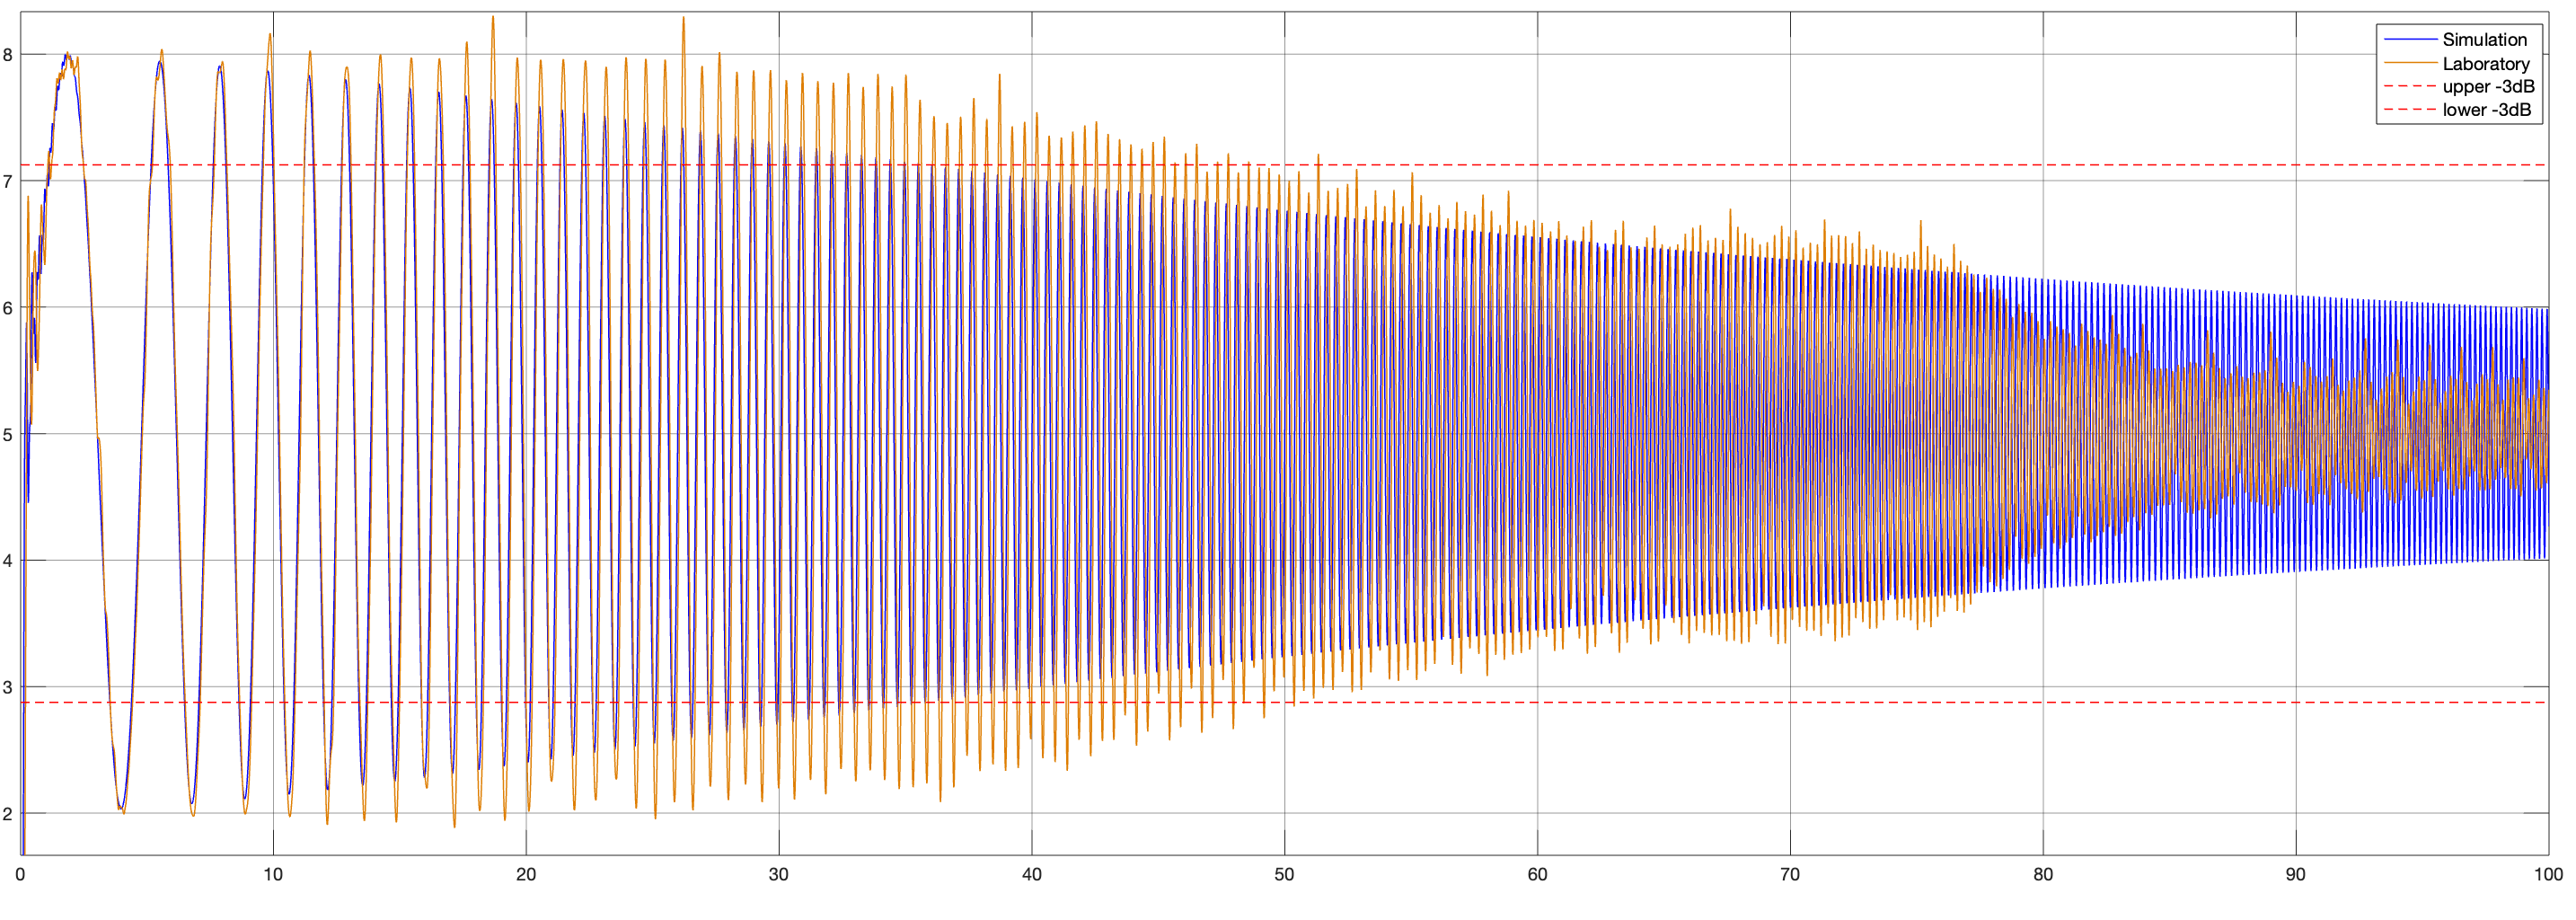
\includegraphics[width=\textwidth]{sine_PI}
	\caption{Sine-sweep experiment from $1\ Hz$ to $10\ Hz$ in $100\ s$}
	\label{fig:sinesweep_speed_2dof}
\end{figure*}

The simulations indicates the cutting frequency around~$11.8\ rad/s$. Data collected in laboratory show a resonance effect at that frequency; as in the case of step response, this could be explained by a lower phase margin in the real system with respect to the simulated one.
Looking at the step response in \cref{fig:step10_noPF}, the overshoot is about~$48\%$, then the \cref{eq:phase_margin_compute} gives phase margin of about~$25\degree$.

Actually, another difference arises at about~$75\ s$, that corresponds to a frequency around~$25\ rad/s$: at this frequency, there is the first resonance peak of the plant. An explanation to this different behavior could be an under-estimation of the damping coefficient in model identification: by applying a too strong damping coefficient to the zeros of the notch filter, it generates a small decreasing of the modulus at that frequency to the overall system. As consequence, the whole resonance peak has been compensated more than needed and the sine-sweep experiment shows it very well. \\

As it has been done for the \onedof\ system, the range of reachable set-points is tested with a ramp with decreasing low speed. In this case, the presence of small oscillations prevents the control the system at very low speed. For this reason the controllable speed belongs to two possible intervals: from~$-17\ rad/s$ to~$-0.5\ rad/s$ and from~$0.5\ rad/s$ to~$17\ rad/s$.
\begin{figure*}[h]
	\centering
	\begin{subfigure}{0.45\columnwidth}
		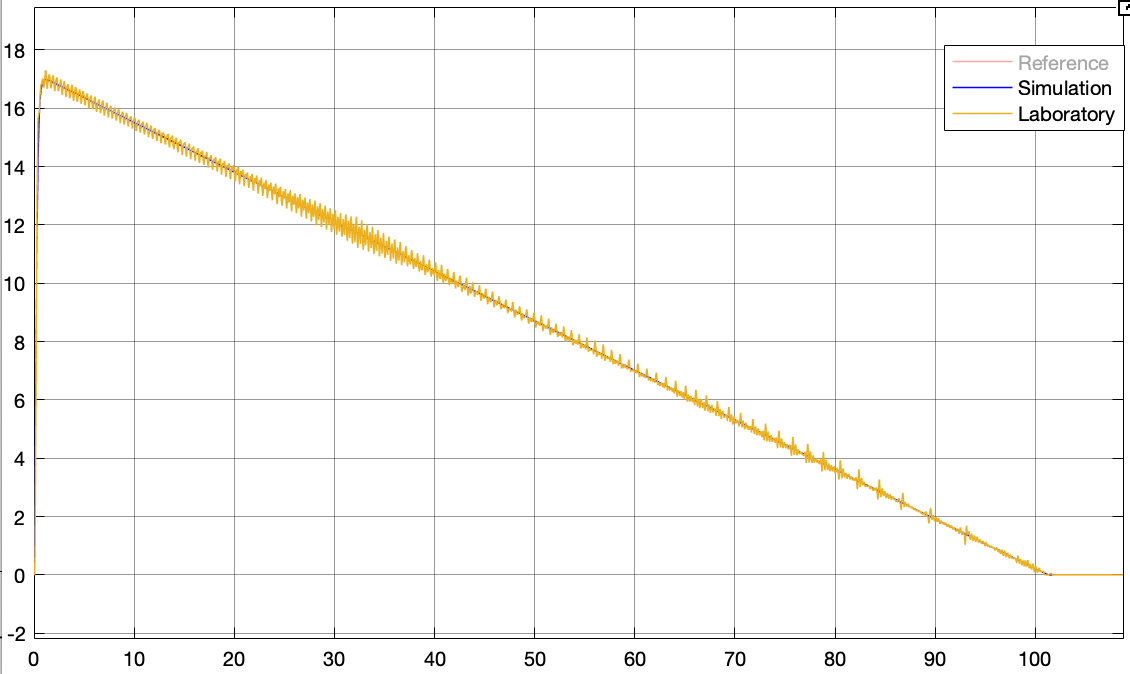
\includegraphics[width=\textwidth]{Ramp2dofa}
		\subcaption{Entire experiment}
	\end{subfigure}
	\begin{subfigure}{0.45\columnwidth}
		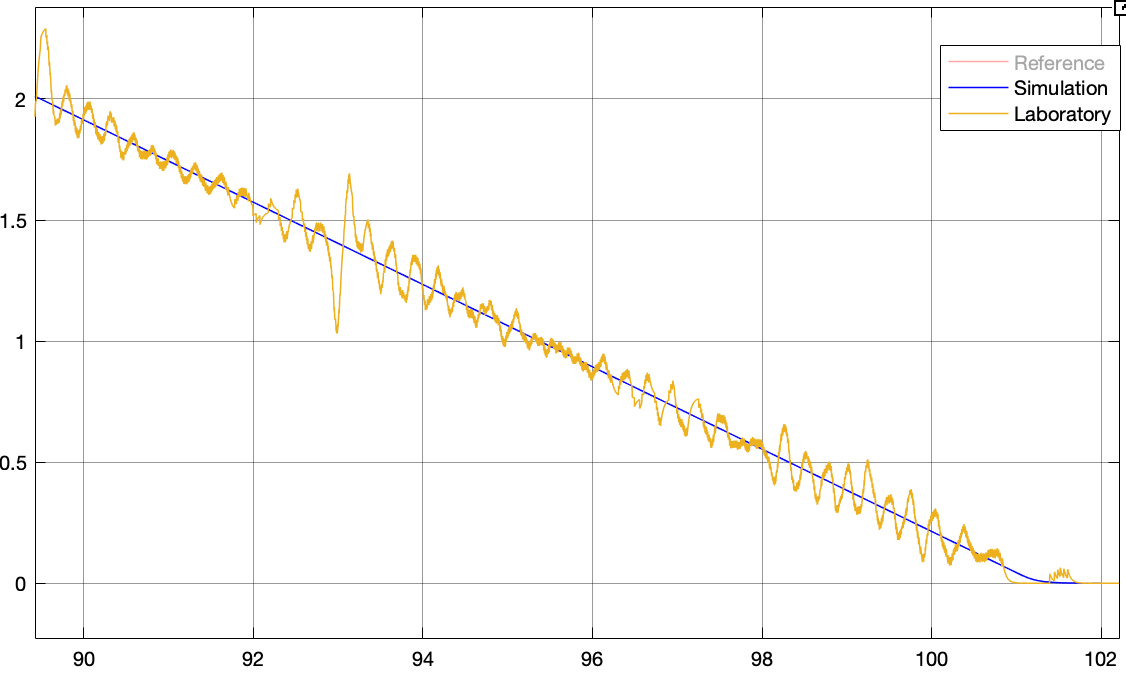
\includegraphics[width=\textwidth]{Ramp2dofb}
		\subcaption{Detail at low speed}
	\end{subfigure}

	\caption{Ramp experiment from $17\ rad/s$ to $0\ rad/s$ in $100\ s$}
	\label{fig:Ramp2dof}
\end{figure*}

\newpage
\subsection{Position Control Loop}

Following the same reasoning of the \onedof~case, a cascade control strategy is used. The low-pass filter solution in the inner loop is avoided, because of the change of the scheme: the reference signal does not enter directly to the speed closed loop, but the speed reference is now generated by the proportional gain of the outer loop. On the other hand, the inner loop without pre-filter leads to a more oscillating dynamic. 

\begin{figure*}[h]
	\centering
	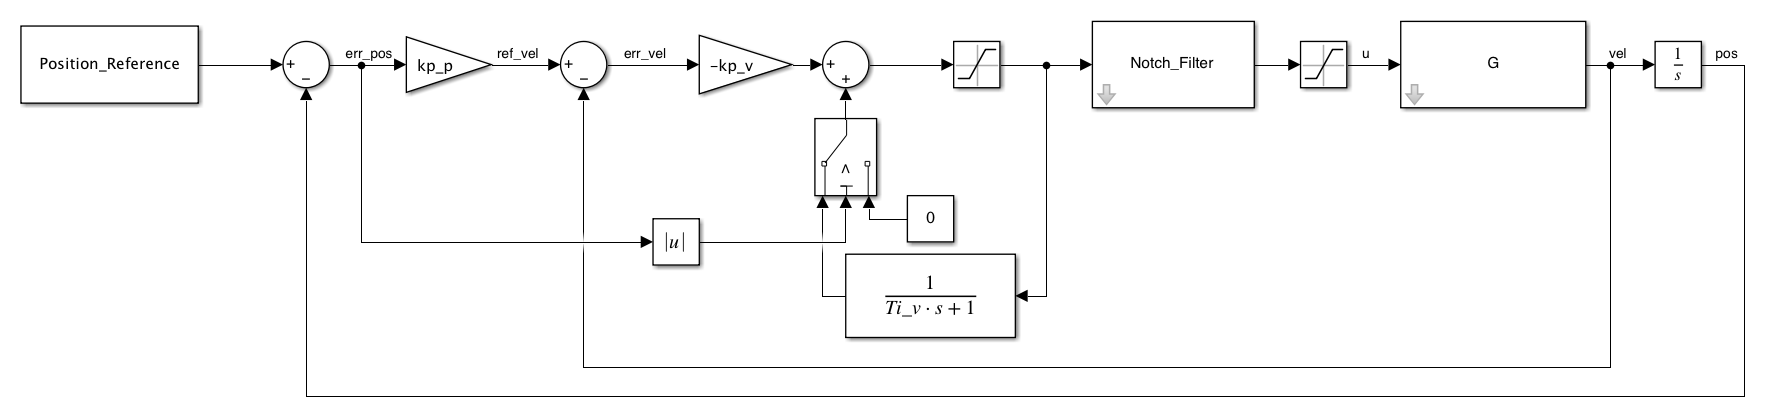
\includegraphics[width=0.8\textwidth]{1dof_P_scheme}
	\label{fig:Closed-loop block scheme2}
	\caption{Closed-loop block scheme}
\end{figure*}

\paragraph{Tuning and simulation}
A comparison between three different solutions is now provided:
\begin{itemize}
	\item $k_v=5$ and $k_p=3$
	\item $k_v=5$ and $k_p=2.5$
	\item $k_v=4$ and $k_p=2$
\end{itemize}
where $k_v$ represents the gain used to set the PI regulator of the inner loop, while~$k_p$ is the gain of position loop. For the reason that each solution has a different~$k_p$, from now on only~$k_p$ will be used to distinguish them.
\begin{figure*}[h]
	\centering
	\begin{subfigure}{0.4\columnwidth}
		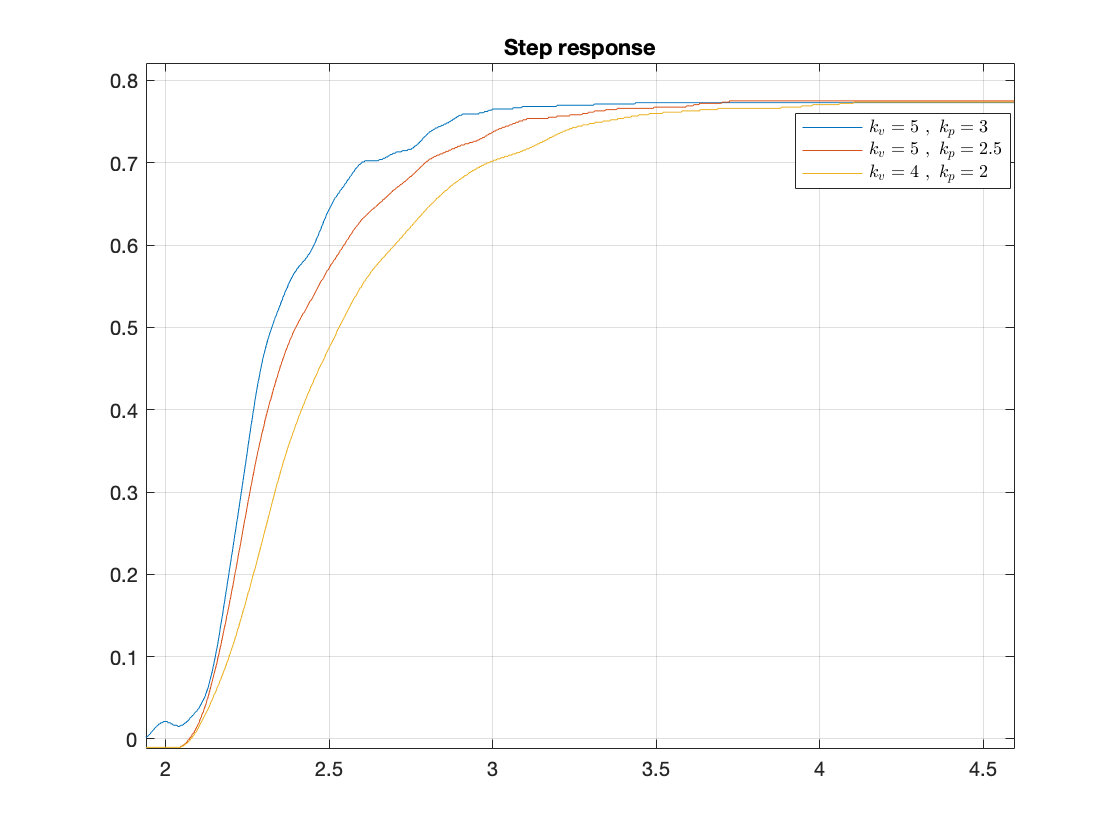
\includegraphics[width=\textwidth]{2dof_P_comparison}
		\subcaption{Closed-loop step responses}
		\label{fig:P2dof_step}
	\end{subfigure}
	\begin{subfigure}{0.4\columnwidth}
		\begin{tabular}{|c|ccc|}
			\hline
			Results\footnote{Gain margin~$G_m$ and phase margin~$\phi_m$ are obtained theoretically by means of MATLAB. Instead, settling time~$T_s$ is measured through data collected at the laboratory.} & $k_p=3$ & $k_p=2.5$ & $k_p=2$ \\
			\hline
			$G_m\ [dB]$ & $20.4$ & $22$ & $24.1$ \\
			$\phi_m\ [deg]$ & $70.5$ & $73.6$ & $73.7$ \\
			\hline
			$T_s\ [s]$ & $0.90$ & $1.25$ & $1.75$ \\
			\hline
		\end{tabular}
	\end{subfigure}
	\caption{Comparisons between $k_p=2$, $k_p=2.5$ and $k_p=3$ cases}
	\label{fig:Bode and Step P 2dof comparison}
\end{figure*}

From the comparison done in \cref{fig:Bode and Step P 2dof comparison}, it can be notice that the best solution is provided by imposing $k_v=5$ and  $\omega_{c,p}=3$. Indeed, it has the smallest settling time, but at the same time it keeps a completely acceptable phase margin. By comparing each of this solution with its respective simulation, we noticed how in both cases with $w_{c,p}=3$ and $w_{c,p}=2.5$, the simulation is quite different from the data collected at the laboratory. While as regards the third scenario, this difference is almost negligible. Since we favored the great simulation reliability of this last case over the low settling time of the case given by $w_{c,p}=3$, it has been chosen as the optimal solution the one obtained by imposing $k_v=4$ and $\omega_{c,p}=2$.

\paragraph{Performance analysis}
Below, it possible to see the comparison between simulation and laboratory data obtained with this control strategy.
\begin{figure*}[h]
	\centering
	\begin{subfigure}{0.48\columnwidth}
		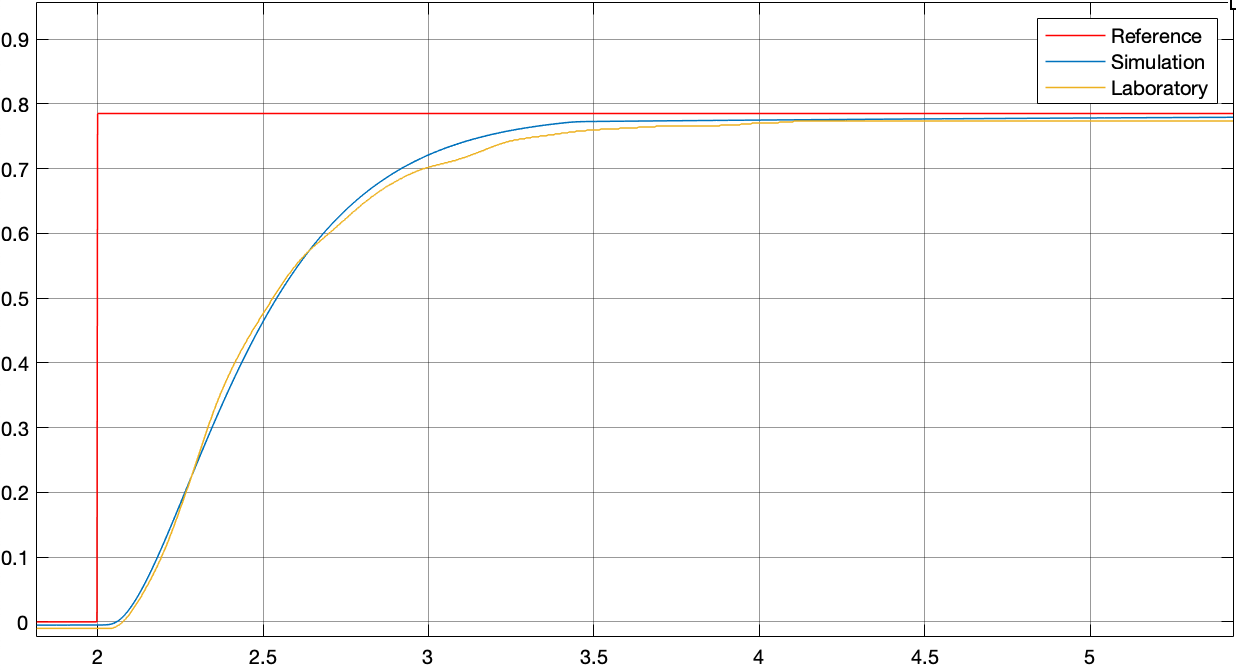
\includegraphics[width=\textwidth]{step_P_2dof}
		\subcaption{Position}
		\label{fig:P_2dof_pos}
	\end{subfigure}
	\begin{subfigure}{0.45\columnwidth}
		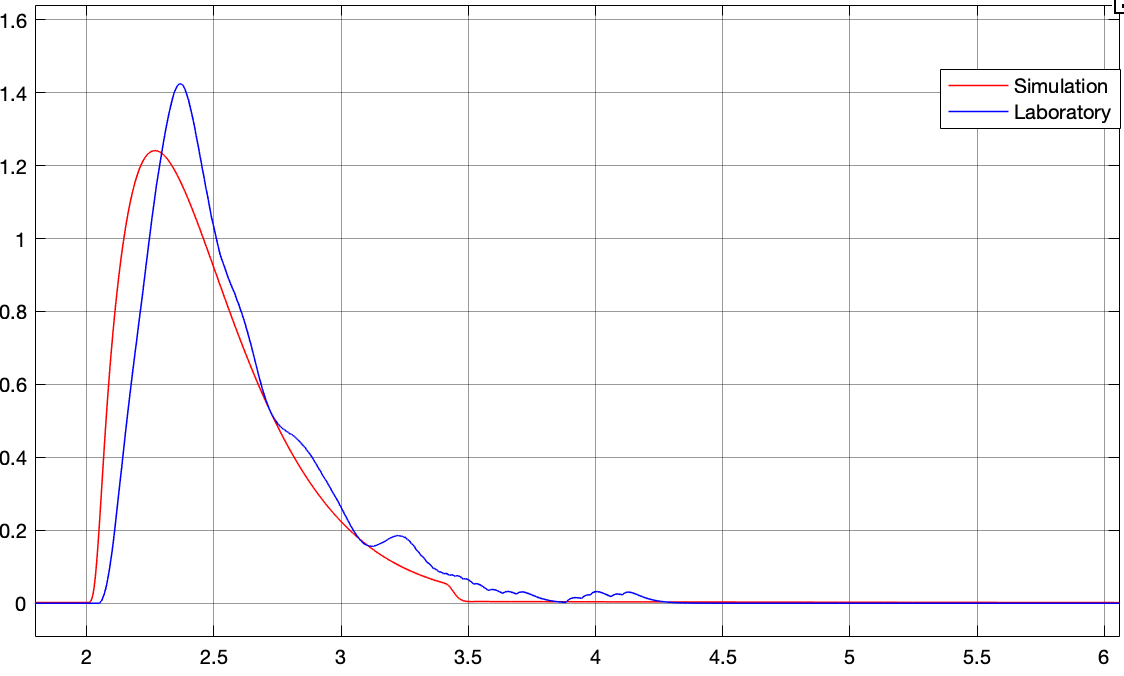
\includegraphics[width=\textwidth]{speed_P_2dof}
		\subcaption{Speed}
	\end{subfigure}
	\begin{subfigure}{0.45\columnwidth}
		\includegraphics[width=\textwidth]{volt_P_2dof}
		\subcaption{Voltage}
		\label{fig:P_2dof_volt}
	\end{subfigure}
	\caption{Position control loop with $k_{p} =2$ with a position step of $\frac{\pi}{4}\ rad$}
\end{figure*}

The settling time is around~$1.75\ s$, that is considered satisfactory. \\
From \cref{fig:P_2dof_volt}, it can be observed the presence of two voltage spikes, which do not influence neither the position nor the mass speed. As done in the \onedof\ position control, a logic switch is inserted in the PI controller to overcome the static friction issue by disabling the integrator. This switch might be the cause of those spikes, indeed, these events arise whenever the switch is activated. \\
It is possible to notice in \cref{fig:P_2dof_pos}, that the second mass does not reach the position reference due to the above-mentioned switch gate.

\paragraph{Bandwidth and phase margin estimation}
The mismatch between simulation and laboratory data is fully negligible, as it is shown through the sine-sweep experiment in \cref{fig:sinesweep_pos_2dof}. From this, it can be seen that the bandwidth of the closed-loop system has been estimated to be equal to~$w_{c,p}=2.7$, both for the simulation and the laboratory data. This result is also confirmed by the closed-loop Bode diagram (\cref{fig:2dof_pos_bode}) and by step response settling time.
The simulation accuracy with respect to the real system suggests that also the phase margin computation is almost correct: $\phi_m = 73.7\degree$.
\begin{figure*}[h]
	\centering
	\begin{subfigure}{0.45\columnwidth}
		\includegraphics[width=\textwidth]{openloop_margin_pos_2dof}
		\subcaption{Open-loop Bode diagram}
	\end{subfigure}
	\begin{subfigure}{0.45\columnwidth}
		\includegraphics[width=\textwidth]{closedloop_bode_pos_2dof}
		\subcaption{Closed-loop Bode diagram}
		\label{fig:2dof_pos_bode}
	\end{subfigure}
	\begin{subfigure}{0.9\columnwidth}
		\includegraphics[width=\textwidth]{sine_P_2dof}
		\subcaption{Sine-sweep experiment from $0.1\ Hz$ to $1\ Hz$ in $100\ s$}
		\label{fig:sinesweep_pos_2dof}
	\end{subfigure}
	\caption{Bode and sine-sweep analyses}
\end{figure*}
	\chapter{State reconstruction}
		
In next chapters, more advanced control techniques will be treated. All of them are based on the state-space realization of the system, so a reconstruction of the state is needed since some signals are not available because too noisy to be used (i.e. motor and masses speed, derived by potentiometer and encoders position readings).

\section{State observer}

The gray-box models, identified in \cref{sec:gray_b_id}, are sufficiently precise to be used for observers design. The state reconstruction is performed by using motor and masses position signals; poles of the closed-loop observer are placed in a prescribed position: they must be sufficiently far from the imaginary axis so that asymptotic stability is ensured~(even considering poles uncertainty) and, moreover, time settlement of the observer is satisfactorily low.

\paragraph{\onedof\ system}

In order to construct the observer, matrices A and C are needed~(where C matrix identifies the available signals, paying attention to those sign). In case of \onedof\ system:

\begin{equation}
	A = 
	\begin{bmatrix}
		0 &1 & 0 & 0 \\
		-\frac{K_{s_1}}{J_m} & -\frac{B_m}{J_m}-\frac{\eta_m \eta_g k_t k_m {K_g}^2}{R_m J_m}  & \frac{K_{s_1}}{J_m} & 0 \\
		0 & 0 & 0 & 1 \\
		\frac{K_{s_1}}{J_1} & 0 & -\frac{K_{s_1}}{J_1} & -\frac{B_1}{J_1}
	\end{bmatrix}
	\qquad
	C =
	\begin{bmatrix}
		1 & 0 & 0 & 0 \\
		0 & 0 & -1 & 0
	\end{bmatrix}
\label{eqn:1dof_mat_obs}
\end{equation}

Closed-loop poles can be automatically placed in prescribed positions thanks to the MATLAB function~\textit{place}\footnote{This function requires to locate poles in different positions. To place poles in a unique position, it is sufficient to slightly move some of them.}.
The choice for poles frequency is~$400 \, rad/s$, meaning that the settling time of the observer is about 12.5 ms.

The estimated state dynamics, then, becomes
\begin{equation}
	\dot{\hat{x}}(t) = A\hat{x}(t) + Bu(t) + L [y(t) - C\hat{x}(t) - Du(t)] = (A-LC)\hat{x}(t) + (B-LD)u(t) + Ly(t)
	\label{eqn:est_state_dyn}
\end{equation}
and its estimation error dynamics is asymptotically stable, as pole placement prescribed:
\begin{equation}
	\dot{\hat{e}} (t) = (A-LC) \hat{e} (t)
\end{equation}

The necessary and sufficient condition to guarantee observer design and asymptotic stability is that pair~$(A,C)$ is observable. In this case, the rank of observability matrix is 4~(as the order of the system). \\

The initial position of the system, detected by the potentiometer, is subtracted to all position readings~(motor, first mass and, if connected, second mass); this causes a shift in state reconstruction that will never be recovered. Actually, this does not represent a problem since this kind of observer is only used for pole-placement controllers: as shown later, this will automatically bring the system to the correct reference thanks to an integral action.\footnote{Just for graphical reasons, reconstructed and real states are superimposed by adding again the initial condition to~$\hat x$.}

In \cref{fig:observer_1dof}, a position control (performed by pole-placement, introduced in next chapter) is reported. It can be seen that the position of motor and first mass are shifted with respect to their measurements because of the initial position; however, position reconstructions perfectly superimpose measurements, as expected.\\
Concerning the speeds, mass velocity is a bit different from the measured one~(derived by the encoder), while motor speed is noisy because of potentiometer high variance; in any case, small differences on speed are not critical, since speed signals are not significantly weighted in next control techniques.

\paragraph{\twodof\ system}

Actually, the \twodof\ observer structure is very similar to the previous one; matrices dimensions and available signals are different: in this case, in addition to potentiometer and first mass encoder, also the second mass position is available thanks to the last encoder. This means that matrix C has one more row:
\begin{equation}
	A = 
	\begin{bmatrix}
		0 &1 & 0 & 0 & 0 & 0 \\
		-\frac{K_{s_1}}{J_m} & -\frac{B_m}{J_m}-\frac{\eta_m \eta_g k_t k_m {K_g}^2}{R_m J_m}  & \frac{K_{s_1}}{J_m} & 0 & 0 & 0 \\
		0 & 0 & 0 & 1 & 0 & 0 \\
		\frac{K_{s_1}}{J_1} & 0 & -\frac{K_{s_1}+K_{s_2}}{J_1} & -\frac{B_1}{J_1} & \frac{K_{s_2}}{J_1} & 0 \\
		0 & 0 & 0 & 0 & 0 & 1 \\
		0 & 0 & \frac{K_{s_2}}{J_2} & 0 & -\frac{K_{s_2}}{J_2} & -\frac{B_2}{J_2}
	\end{bmatrix}
	C =
	\begin{bmatrix}
		1 & 0 & 0 & 0 & 0 & 0 \\
		0 & 0 & -1 & 0 & 0 & 0  \\
		0 & 0 & 0 & 0 & -1 & 0
	\end{bmatrix}
\label{eqn:2dof_mat_obs}
\end{equation}

This time, poles have been located in different positions: 2 of them in~$-300 \, rad/s$ and the other 4 in~$-400 \, rad/s$. Also in this case, $\mathit{O}$ matrix of the pair~$(A,C)$ is full rank. As in the~\onedof\ case, a comparison between measured and reconstructed signals (figure~\ref{fig:observer_2dof}) shows that positions are very precisely estimated, while speeds are noisy and shifted in time.

\begin{figure*}
	\centering
	\begin{subfigure}{0.45\columnwidth}
		\includegraphics[width=\textwidth]{observer_1dof}
		\subcaption{\onedof case}
		\label{fig:observer_1dof}
	\end{subfigure}
	\begin{subfigure}{0.45\columnwidth}
		\includegraphics[width=\textwidth]{observer_2dof}
		\subcaption{\twodof\ case}
		\label{fig:observer_2dof}
	\end{subfigure}
	\caption{Observer reconstruction compared to available measurements}
\end{figure*}

\section{Kalman filter}

The state reconstruction based on Luenberg observer works fine in absence of any disturbance. Unfortunately, as mentioned in \cref{sec:sensors}, sensors produce signals at each sampling time that can be considered as stochastic variables. These variables have a variance that depends on the intrinsic characteristic of the sensors. The solution to represent this kind of behavior, consist in separating the measurement signal $y(t)$ in a component deriving from the states, that can be considered the real value, and a component due to a white noise with a given covariance.  \\

With a mathematical description 

\begin{equation}
	\begin{cases}
		\dot x(t) =\ A x(t) + B u(t) +n_x(t) \\
		y(t) =\ C x(t) + D u(t) + n_y(t)
	\end{cases}
\end{equation}
where $n_x$ and $n_y$ are independent zero-mean white Gaussian processes having covariances
\begin{center}
	$E[n_x(t)n_x'(t)]=Q_x \delta(t-s)$  and $E[n_y(t)n_y'(t)]=Q_y \delta(t-s) $
\end{center}
for some $Q_x = Q_x' \geq 0$ and $Q_y = Q_y' > 0$, where $E[v]$ denotes the expected value of a random variable $v$.\\

The stationary version of the Kalman filtering problem can be posed as the task of generating a reconstruction $\hat x (t)$ of the state vector $x(t)$ using measurement $y(t)$ that minimize 
\begin{equation}
	\lim_{t \to \infty }E[ ||x(t) - \hat x(t) ||^2 ]
\end{equation}
which is the steady state variance of the reconstruction error $ x-\hat x$.\\

Although the original estimation problem didn't take in account any measured input $u$, in presence of it, it is possible to slightly modify the equations for the estimation. 
The estimated state dynamics is a stable and causal LTI system, with equation as \cref{eqn:est_state_dyn}. \\
The $L$ gain is the result of the filtering problem, for the generalized plant, without input $u$.
To obtain it, exogenous input $w$, that is any zero-mean unit-intensity white process such that
\begin{equation}
	\begin{bmatrix}
		n_x(t) \\
		n_y(t)
	\end{bmatrix} = 
	\begin{bmatrix}
		B_wB_w'& B_wD_w'\\
		D_wB_w' & D_wD_w'
	\end{bmatrix} w(t)
\end{equation}
is defined. \\

Under the assumption that noises $n_x$ and $n_y$ are uncorrelated, i.e. $B_wD_w' = 0$, the $L$ matrix is obtained solving a Riccati equation, involving also the other system matrices, that is
\begin{equation}
	Y = AYA' + B_wB_w' + (AYC'+B_wD_w')(CYC'+D_wD_w')^{-1}(CYA'+D_wB_w')
	\label{eqn:riccati_kf}
\end{equation}
where $Y = Y' \geq 0$.\\
Then, 
\begin{equation}
	L = (AYC'+B_wD_w')(CYC'+D_wD_w')^{-1}
	\label{eqn:kf_gain}
\end{equation}

\paragraph{Full sensors use}
Given the above definition of the problem, the \onedof. and the \twodof\ systems generate similar solutions and make use of the same matrices as in \cref{eqn:1dof_mat_obs} and \cref{eqn:2dof_mat_obs}.
The $Q_y$ matrix is defined based on the variances computed at \cref{sec:sensors} and it is kept constant through all the development of this tool. 
On the other hand, matrix $Q_x$ doesn't depend directly on some physical properties and can be used to tune the filter. 
This means that by varying the parameters in this matrix, the solutions of the filtering problem change. \\
Moreover, this matrix can be considered as the uncertainty derived from the model identification process, i.e. since matrices $A$ and $B$ of the system have been computed by grey-box estimation (\cref{sec:gray_b_id}), they are naturally uncertain as they can't capture the real dynamic of the system that is much more complicated. \\

The obtained model can simulate much better the position of the masses then that of the motor shaft, this because during the identifcation process those measurements where taken with the encoder, that is much more accurate than the potentiometer. This translates in a higher value of the state variance for the shaft position then that of the masses. With a similar reasoning, speed states are more uncertain then position ones, as they are derived from them. Trying to balance the filter reliabilty (keeping $Q_x$ as high as possible) and filter settling time (keeping $Q_x$ as low as possible) these are the matrices that better suit the filtering problem.
\begin{equation}
	B_w = \begin{bmatrix}
		0.3e-4 & 0 & 0 & 0 & 0 & 0\\
		0 & 1e-2 & 0 & 0 & 0 & 0 \\
		0 & 0 & 1e-8 & 0 & 0 & 0  \\
		0 & 0 & 0 & 1e-4 & 0 & 0
	\end{bmatrix} \
	D_w = \begin{bmatrix}
		0 & 0 & 0 & 0 & 1e-6 & 0\\
		0 & 0 & 0 & 0 & 0 & 2e-8 
	\end{bmatrix} 
	\label{eqn:b_w_d_w}
\end{equation}
For the \twodof\ system the matrices have the same values, but their size is extended.\\
The results of \cref{eqn:riccati_kf} and \cref{eqn:kf_gain} place the poles of the filters in positions where the dominant time constants are around $0.02\ s$, that is fast enough for our settling time goals. \\

From an analysis of the reconstructed states, it emerges that indeed these are less sensitive to measurement noise then the observers solution. This reflects in improved control signals when state feedback control law are used. \\

Moreover, while the characteristic of the encoder, that is a direct measurement coming from a digital sensor, it is constant through the whole revolution, the one from the potentiometer, that is an indirect measurement from an analog sensor, it is less reliable and limited to some range. 
\begin{figure*}[h]
	\centering
	\includegraphics[width=0.6\columnwidth]{kf reconstruction 2dof.png}
	\caption{Kalman filter reconstruction compared with available measurements}
	\label{fig:kf_2dof}
\end{figure*}
In \cref{fig:kf_2dof} it is possible to see how, despite a drift in the potentiometer measurement around the second step, the reconstructed state is more related to the measurement coming from the encoders than that of the potentiometer. Indeed, the dashed lines (the reconstructed signals) are very close to the signals coming from the encoders (red and green continuous lines), despite the fact that the measurement coming from the potentiometer reaches a different steady state value (continuous blue line). This error in the potentiometer measurement can be the result of a small non linearity in the characteristic of the sensor. \\

This example shows perfectly the reliability of the Kalman filter; the noise variance of the shaft measurement is 50 times bigger than that of the encoders, the solution obtained with this formulation of the problem filters the noise in the optimal way. Moreover, in this specific situation, Kalman filter makes the measurement less reliable almost useless, trusting only the best ones. 

\paragraph{Faulty sensor estimation}
The setup that has been used up to this point has been making use of all  the possible measurements, but after the analysis of the reconstructed state with the Kalman filter there was still a point to be analyzed. What would be the performance and the reliability of the system in case the encoder, that is the most important measurement, doesn't work anymore. \\
This actually happened for real during some laboratory experiment; the encoder from the second mass disconnected from the shaft and couldn't produce any results for some time. \\ 

Thus, for both systems, different state re-constructors have been developed, always based on Kalman filtering and using different combinations of the available sensors. \\
The element that change in the design of the different filters are the matrices $C$ and $D_w$. Based on the combination of sensors, different rows of the original $C$ and $D_w$ matrices are selected. \\
From a first analysis, all the possible setups produce an observable system, thus, applying Kalman filter with the minimum number of sensor is possible in every configuration. \\

The results that are produced from these configurations can be summarized in two types. \\ 

The first can be called encoder based solution, this means that even if the measurement from the potentiometer is available, it is almost automatically discarded in favor of the encoder one. As previously mentioned, this happens because the potentiometer variance is much more bigger then that one of the encoder and Riccati equations produce results that depends mostly on the lowest one. All the solutions where at least one encoder is used, produce this result and generate a state estimator with a time constant very low, allowing to push the control action to high speeds.\\

On the other hand, the solution that makes use of only the potentiometer, both in \onedof\ and \twodof, generates a different type of filter. When only the potentiometer is used, the system matrices for the output equation (example is based on \twodof) becomes 
\begin{equation}
	C = \begin{bmatrix}
		1 & 0 & 0 & 0 & 0 & 0
	\end{bmatrix} \
	D_w = \begin{bmatrix}
		0 & 0 & 0 & 0 & 0 & 0 & 1e-6 & 0 & 0 \\
	\end{bmatrix} 
\end{equation}
The Riccati equation that solves the filtering problem for this system produce much slower re-constructors. The time constant of the produced filter is around~$0.8\ s$. Changing the parameters in the matrix $Q_x$ allows to steer a little bit the position of the poles of the estimator, but it can't move a lot the time constant of the main dynamic, mainly its damping. Indeed, the matrix $B_w$ at \ref{eqn:b_w_d_w} has been selected with those values because it was the one generating the less oscillatory response of the filter for this setup and a fast enough estimation for the other ones.\\

In order to be able to use also this setup the control action needs to be slowed down, otherwise different controllers should be tuned based on the availability of the sensors and logic switches could select the more appropriate controller.\\

Some tests with a switch that selects the different state re-constructors have been performed. The results are not satisfying. In the \onedof\ setup, when the controller passes from the Kalman filter with all the sensors to the one with only the encoder, this isn't a problem and the system keeps following the reference, but when it starts to use the estimation derived only by the potentiometer, it diverges. This diverging behavior is not caused by an unstable mode of the controller, but it is due to a couple of reasons. When the controller is switched the estimation changes instantaneously and so does the control action. When the two estimates are quite closed, like between the classic filter and the one with only the encoder, this sudden change results in a very small step in the voltage applied. Instead, when the estimations differ a lot, this voltage step may be too big and the saturation block limits the control action. This triggers an unstable effect, with the voltage being applied continuously at the two saturation limits. The controller is unable to revert this, trying to apply bigger and bigger control actions to bring the state back to reference, but being limited by the saturation block. To avoid this effect, that couldn't be compensated in an easy way, the observers have been tested one at the time. \\

The results confirm partially the hypothesis, the filters with at least one encoder for the \onedof\ and at least~2 sensors for the \twodof\ system works well and can use the fastest controller.\\
Moreover, the \onedof\ system can be controlled estimating the states from only the potentiometer measurement, but with the condition of slowing down the controller.\\

On the other hand, for the \twodof\ setup it was not possible to control it using only the potentiometer, despite being able to reconstruct the states using only one of the two encoders.
In this case the reason is not completely caused by the high variance of the sensor, but it can be found in the observabilty matrix. This is full rank for all the possible combination of used measurements, but this result is obtained numerically on MATLAB. This means that even a small difference in the order of a thousands between the eigenvectors will produce a full rank matrix, so the rank analysis is not completely reliable. \\ 

To grasp this aspect, the following procedure has been followed. The rank of a matrix is the number of linearly independent eigenvectors.
\label{SVD_explaination}
Using SVD, it possible to extract the eigenvectors of a matrix. This method is applied to the observabilty matrix of different configurations. The numbers in the eigenvectors of the observability matrix smaller then a thousand can be neglected and therefore they are set to zero. For the setups using only the encoders or more than one sensor the remaining vectors are clearly linearly independent (each couple of vectors has just 2 elements different from zero), while for the \twodof\ system using only the potentiometer they appear to be more involved (there are some vectors that have up to 4 elements different from zero), hence they are not perfectly linearly independent.
Here it is possible to see the result of this analysis for the eigenvectors of the observality matrix of the \twodof\ system with only the encoder on the last mass or with only the potentiometer. 
\begin{equation}
	e_{O_{\theta_{2}}}= \begin{bmatrix}
		0& 0 & 0 & 0 		& -0.708 & -0.706 \\
		0& 0 & 0 & 0.002 &  0.706 & -0.708 \\
		0& 0 & -0.389 & -0.921 & 0 & -0.002 \\
		0& 0 & -0.921 & -0.389 & 0 & 0 \\
		0.235 & -0.972 & 0 & 0 & 0 & 0 \\
		-0.972 & -0.235 & 0 & 0 & 0 & 0 \\
	\end{bmatrix}
\end{equation}
\begin{equation}
	e_{O_{\theta_{l}}}= \begin{bmatrix}
		0& 0 & 0 & -0.006  & 0.751 & 0.661 \\
		0& 0 & 0 & 0.096 &  -0.657 & 0.748 \\
		0& 0.002 & -0.031 & -0.995 & -0.068 & 0.068 \\
		0& -0.084 & 0.996 & -0.031 & -0.002& 0.002 \\
		-0.022 & 0.9963 & 0.084 & 0 & 0 & 0 \\
		0.999 & 0.022 & 0.002 & 0 & 0 & 0 \\
	\end{bmatrix}
\end{equation}

	\chapter{Pole placement}
	  	
After we have shown a set of possible solutions with the frequency controllers, we provide now an approach in the state-space domain. This is possible thanks to the estimations made through the \textit{greyest} function by Matlab.\\
As shown in the previous chapter, we have built a full-state observer and kalman filters with different input sensor configurations, in order to simulate the reliability of the controller with respect to eventual faults. We will introduce now a pole placement technique taking as input the estimated states coming out from observer or kalman filters. Later, we will compare these solutions and we will choose the optimal configuration. The \textit{1-DOF} case will be analyzed at first and then we will study the \textit{2-DOF} one.

\section{1-DOF}
The estimated states are so $\hat{\theta_{l}}$, $\hat{\dot{\theta_{l}}}$, $\hat{\theta_{1}}$,  $\hat{\dot{\theta_{1}}}$. 
A pole placement applied to the only four states of the system is not sufficient to reach the reference; to overcome this problem we decided to apply an integrator. A possible solution is to enlarge the system, adding a state $v(t)$; the resulting enlarged state space system is the following one:

\begin{equation}
	\begin{bmatrix}
		\dot\theta_l \\
		\ddot\theta_l \\
		\dot\theta_1 \\
		\ddot\theta_1 \\
		\dot{v}
	\end{bmatrix}
	=
	\begin{bmatrix}
		0 &1 & 0 & 0 & 0 \\
		-\frac{K_{s_1}}{J_m} & -\frac{B_m}{J_m}-\frac{\eta_m \eta_g k_t k_m {K_g}^2}{R_m J_m}  & \frac{K_{s_1}}{J_m} & 0 & 0 \\
		0 & 0 & 0 & 1 & 0 \\
		\frac{K_{s_1}}{J_1} & 0 & -\frac{K_{s_1}}{J_1} & -\frac{B_1}{J_1} & 0 \\
		0 & 0 & 1 & 0 & 0 
	\end{bmatrix}
	\begin{bmatrix}
		\theta_l \\
		\dot\theta_l \\
		\theta_1 \\
		\dot\theta_1 \\
		v
	\end{bmatrix}
	+
	\begin{bmatrix}
		0 \\
		\frac{\eta_m \eta_g k_t K_g}{R_m J_m} \\
		0 \\
		0 \\
		0
	\end{bmatrix}
	V
\end{equation}

Now we check the controllability of this enlarged system by using \textit{ctrb} Matlab function.
As exepcted it is fully controllable and now we can proceed by using the following scheme:
\begin{figure*}[h]
	\centering
	\includegraphics[scale=0.3]{pp_1}
	\caption{block scheme with pole placement and state reconstraction}
	\label{fig:block scheme with pole placement and state reconstraction}
\end{figure*}

% \newpage

In figure \ref{fig:block scheme with pole placement and state reconstraction}, the state estimator block represents either the observer or one of the Kalman filters. 
At this point we set the poles through the \textit{place} matlab function. In particular we decide to postpone the real poles to speed up the system, whereas concerning the complex ones we just enhance their damping coefficients. At the beginning we thought to turn them into real poles but the resulting control effort was very aggressive and it was not leading any significant improvement to the dynamics. The placed poles and the corresponing gain $K$ computed by the above-mentioned matlab function are written below:
\\\\

\begin{equation}
	PlacedPoles^{T} =
	\begin{bmatrix}
		-20 \\ -50 \\ -40.1*(0.8+\sin(\arccos(0.8))*i) \\ -40.1*(0.8-\sin(\arccos(0.8))*i) \\-10  
	\end{bmatrix}
	K_x^{T} =
	\begin{bmatrix}
		185.9405 \\  3.5059 \\ -125.8645 \\   0.1222
	\end{bmatrix}
	\\
	K_v =
	\begin{bmatrix}
		286.2122
	\end{bmatrix}
\end{equation}

We will provide now the comparison between the configurations made by the same pole placement and the different state estimator. We will do it plotting also the simulation made through our scheme. Doing so we test the reliability of our model with respect the real system.

\begin{figure*}[h]
	\centering
	\begin{subfigure}{0.45\columnwidth}
		\includegraphics[scale=0.55]{response_pp_1}
		\caption{Position}
	\end{subfigure}
	\begin{subfigure}{0.45\columnwidth}
		\includegraphics[scale=0.565]{voltage_pp_1}
		\caption{Voltage}
	\end{subfigure}
	\caption{Position step response with full-state observer}
	\label{fig:Position step response with full-state observer}
\end{figure*}

\begin{figure*}[h]
	\centering
	\begin{subfigure}{0.45\columnwidth}
		\includegraphics[scale=0.33]{kf1_pp_1}
		\caption{Position}
	\end{subfigure}
	\begin{subfigure}{0.45\columnwidth}
		\includegraphics[scale=0.33]{kf1_pp_2}
		\caption{Voltage}
	\end{subfigure}
	\caption{Position step response with full Kalman filter (potentiometer and enconder)}
	\label{fig:Position step response with full Kalman filter}
\end{figure*}

As regards the step response, we can notice as the Kalman filter configuration is not as smooth as the observer one. This might be caused by a delay in Kalman Filter state estimation. By the way, both cases are considered acceptable. On the other hand, the Kalman filter brings a significant improvement on the control action, resulting to be less noisy due to the filter robustness against the white noises.
We are already satisfied by this performance and we do not need to speed it up, however other solutions will be provided later on with LQG.

\section{2-DOF}
As before, we enlarge the system in order to reach the position reference. The overall enlarged state space system and the closed control loop scheme are the following ones:

\begin{equation}
	\begin{bmatrix}
		\dot{\theta_l} \\
		\ddot{\theta_l} \\
		\dot{\theta_1} \\
		\ddot{\theta_1} \\
		\dot{\theta_2} \\
		\ddot{\theta_2} \\
		\dot{v}
	\end{bmatrix}
	=
	\begin{bmatrix}
		0 &1 & 0 & 0 & 0 & 0 & 0 \\
		-\frac{K_{s_1}}{J_m} & -\frac{B_m}{J_m}-\frac{\eta_m \eta_g k_t k_m {K_g}^2}{R_m J_m}  & \frac{K_{s_1}}{J_m} & 0 & 0 & 0 & 0 \\
		0 & 0 & 0 & 1 & 0 & 0 & 0\\
		\frac{K_{s_1}}{J_1} & 0 & -\frac{K_{s_1}+K_{s_2}}{J_1} & -\frac{B_1}{J_1} & \frac{K_{s_2}}{J_1} & 0 & 0\\
		0 & 0 & 0 & 0 & 0 & 1 & 0 \\
		0 & 0 & \frac{K_{s_2}}{J_2} & 0 & -\frac{K_{s_2}}{J_2} & -\frac{B_2}{J_2} & 0 \\
		0 & 0 & 0 & 0 & 1 & 0 & 0
	\end{bmatrix}
	\begin{bmatrix}
		\theta_l \\
		\dot{\theta_l} \\
		\theta_1 \\
		\dot{\theta_1} \\
		\theta_2 \\
		\dot{\theta_2} \\
		v 
	\end{bmatrix}
	+
	\begin{bmatrix}
		0 \\
		\frac{\eta_m \eta_g k_t K_g}{R_m J_m} \\
		0 \\
		0 \\
		0 \\
		0 \\
		0 
	\end{bmatrix}
	V
\end{equation}


\begin{figure*}[h]
	\centering
	\includegraphics[scale=0.3]{pp_2}
	\caption{Block scheme with pole placement and state reconstruction}
\end{figure*}

Also in this case, we decide not to force the complex poles to real ones, but we just rise their damping coefficients. Below, it is possible to see where we placed the new poles of the system and the gain vector that lets us do it.

\begin{equation}
	PlacedPoles^{T} =
	\begin{bmatrix}
		-20 \\ -30 \\ -24.5*(0.6+\sin(\arccos(0.6))*i) \\ -24.5*(0.6-\sin(\arccos(0.6))*i) \\
		-61.9*(0.2+\sin(\arccos(0.2))*i) \\ -61.9*(0.2-\sin(\arccos(0.2))*i) \\ -10
	\end{bmatrix}
	K_x^{T} =
	\begin{bmatrix}
		68.1752  \\  1.1393 \\ -71.9542 \\   0.0150 \\  30.2715  \\  0.5489
	\end{bmatrix}
	\\
	K_v =
	\begin{bmatrix}
		110.9516
	\end{bmatrix}
\end{equation}

\begin{figure*}[h]
	\centering
	\begin{subfigure}{0.5\columnwidth}
		\includegraphics[scale= 0.37]{response_pp_2}
		\caption{Position}
	\end{subfigure}
	\begin{subfigure}{0.45\columnwidth}
		\includegraphics[scale=0.25]{voltage_pp_2}
		\caption{Voltage}
	\end{subfigure}
	\caption{position step response with full-state observer}
\end{figure*}

\begin{figure*}[h]
	\centering
	\begin{subfigure}{0.5\columnwidth}
		\includegraphics[scale= 0.37]{2_kf1_1}
		\caption{Position}
	\end{subfigure}
	\begin{subfigure}{0.45\columnwidth}
		\includegraphics[scale=0.37]{2_kf1_2}
		\caption{Voltage}
	\end{subfigure}
	\caption{Position step response with full Kalman filter (potentiometer and two enconders)}
\end{figure*}

\begin{figure*}[h]
	\centering
	\begin{subfigure}{0.5\columnwidth}
		\includegraphics[scale= 0.37]{2_kf2_1}
		\caption{Position}
	\end{subfigure}
	\begin{subfigure}{0.45\columnwidth}
		\includegraphics[scale=0.37]{2_kf2_2}
		\caption{Voltage}
	\end{subfigure}
	\caption{Position step response with Kalman filter (second mass enconder only)}
\end{figure*}

	\chapter{Linear-quadratic regulator}
		
The controller structure derived from this technique is similar to the pole placement one, but a significant conceptual difference exists. In fact, the linear quadratic regulator~(LQR) is obtained by optimizing the cost function~(\ref{eq:LQ_cost_function}) that includes both state and output, weighted by~$Q$ and~$R$ matrices respectively.
\begin{equation}
	J(x_0, u) = \int_{0}^{+\infty} \bigl{[} x'(\tau)Qx(\tau) + u'(t)Ru(t) \bigr{]} \; d\tau
	\label{eq:LQ_cost_function}
\end{equation}

The time horizon is infinite, so the solution~$\bar{P}$ of the \textit{algebraic Riccati equation}~(\ref{eq:LQ_ARE}) is constant and returns the time-invariant control law~(\ref{eq:LQ_control_law}).
\begin{subequations}
	\begin{equation}
		0 = A' \bar{P} + \bar{P} A + Q - \bar{P} B R^{-1} B' \bar{P}
		\label{eq:LQ_ARE}
	\end{equation}
	\begin{equation}
		u(t) = -K x(t)
		\label{eq:LQ_control_law}
	\end{equation}
\end{subequations}

The system response, such as settling time and transient shape, highly depends on mutual ratios between values in those matrices, that become design parameters. Many simulations in Simulink allowed us to find a possible trade-off among those parameters, just to perform an acceptable experiment in laboratory and, starting from that, improve performances by tuning.
As done in pole placement, the system~(both in case~\acrshort{1-dof} and~\acrshort{2-dof}) has been enlarged so that an integrator is able to nullify the steady-state error.

\paragraph{\acrshort{1-dof} system}

Similarly to the pole-placement control, the state is enlarged by adding an integrator on the error:
\begin{equation}
	\begin{bmatrix}
		\dot{x} \\
		\dot{v}
	\end{bmatrix}
	=
	\begin{bmatrix}
		A_{sys} & 0 \\
		-C_{back} & 0
	\end{bmatrix}
	\begin{bmatrix}
		x \\
		v
	\end{bmatrix}
	+
	\begin{bmatrix}
		B_{sys} \\
		0
	\end{bmatrix}
	V
	\qquad
	where \; C_{back} =
	\begin{bmatrix}
		0 & 0 & -1 & 0 & 0
	\end{bmatrix}
\end{equation}

For the design of this control technique, performing simulations is essential to find a good trade-off between~$Q$ and~$R$ values: their balance is fundamental to simultaneously have a rapid smooth transient and negligible steady-state error. A great coefficient on the integral part imposes a fast response and small steady-state error; quite high values on the position variables~($\theta_l$ and~$\theta_1$) accelerate in reaching the equilibrium, i.e.\ the reference. \\ Further considerations about speeds weight are needed: a very small coefficient on~$\dot \theta_l$ and~$\dot \theta_1$ would encourage high-frequency speed variation and then oscillations; on the other hand, augmenting those coefficients would speed-down the response, since a velocity variation~(necessary to move the mass) is discouraged. In conclusion, speeds parameters are probably the most difficult to be found. \\ Matrix~$R$ acts on the control variable usage: a too small coefficient causes rapid oscillations on voltage, a high value imposes a loose control action.
Here the matrices found by simulation:
\begin{equation}
	Q =
	\begin{bmatrix}
		50 & 0 & 0 & 0 & 0 \\
		0 & 0.1 & 0 & 0 & 0 \\
		0 & 0 & 50 & 0 & 0 \\
		0 & 0 & 0 & 0.1 & 0 \\
		0 & 0 & 0 & 0 & 3000 \\
	\end{bmatrix}
	\qquad
	R = 0.8
\end{equation}

The control law, hence, depends on both the state~$x(t)$ and the integral variable~$v(t)$. Since not all measurements are available~(speeds are very noisy), a state reconstructor is necessary: the Kalman Filter introduced in chapter~4 works thanks to~$\theta_l$ and~$\theta_1$ signals, that makes this LQR an LQG control. As shown in figure~\ref{fig:1dof_LQ_classicKF}, from the simulation a settling time of~0.8~s~(comparable to the previous controllers, but greater than the one of Kalman Filter, as desired) is expected. Actually, laboratory experiment is a bit oscillating in the transient; indeed, this control technique does not explicitly cancel the system dynamics, difficult to be attenuated by tuning matrices. At steady-state condition, the integral action could detect a small static error that would cause some sudden motions, so a switch disables the input signal of the integrator in proximity of the reference.

\begin{figure*}
	\centering
	\begin{subfigure}{0.45\columnwidth}
		\includegraphics[width=\textwidth]{1dof_LQ_classicKF}
		\subcaption{LQG with all measurements}
		\label{fig:1dof_LQ_classicKF}
	\end{subfigure}
	\begin{subfigure}{0.45\columnwidth}
		\includegraphics[width=\textwidth]{1dof_LQ_minKF_pot}
		\subcaption{LQG with potentiometer sensor only}
		\label{fig:1dof_LQ_minKF_pot}
	\end{subfigure}
	\newline
	\begin{subfigure}{\columnwidth}
		\centering
		\includegraphics[width=0.9\textwidth]{1dof_LQ_KF_switch}
		\subcaption{LQG with switch among different KF}
		\label{fig:1dof_LQ_KF_switch}
	\end{subfigure}
	\caption{LQG with different sensors available, \acrshort{1-dof} case}
\end{figure*}

\subparagraph{Sensors not available: minimum Kalman Filters}

% verificare concordanza con spiegazione minKF in capitolo 4
Now we consider the case of missing signals, possibly due to sensor faults or installation impossibility. In this case, the Kalman Filters structure changes, as explained in chapter~4. In case the signal of the last mass, here~$\theta_1$, is not available, the reference error is computed on the estimation of that signal~($\hat\theta_1$), figure~\ref{fig:KF_state_feedback}. \\

\begin{figure*}
	\centering
	\includegraphics[width=0.8\textwidth]{KF_state_feedback}
	\caption{State measurement not available: estimated state feedback, \acrshort{1-dof} case}
	\label{fig:KF_state_feedback}
\end{figure*}

In order to speed up the laboratory experience, a long experiment that switches among the different combinations of available sensors has been performed; this simulates a real-time fault detection and, accordingly, commutation to a congruous configuration of the reconstructor.

In the~\acrshort{1-dof} case, actually, there are three different situations: all sensors available (i.e.\~potentiometer and first mass encoder), encoder only~($\theta_l$), potentiometer only~($\theta_1$). Unfortunately, this last Kalman Filter is very slow because of the potentiometer noise, hence an \textit{ad hoc} slower controller must be designed~(settling time~4~s, comparable with the Kalman time response):
\begin{equation}
	Q =
	\begin{bmatrix}
		50 & 0 & 0 & 0 & 0 \\
		0 & 1 & 0 & 0 & 0 \\
		0 & 0 & 50 & 0 & 0 \\
		0 & 0 & 0 & 1 & 0 \\
		0 & 0 & 0 & 0 & 100
	\end{bmatrix}
	\qquad
	R = 0.8
\end{equation}

A switch between the faster and the last one controllers could create some issues: a small error in the state estimation would cause a jump in the control action~(that is determined by a different gain~
$
\begin{bmatrix}
	K_x & K_v
\end{bmatrix}
$), generating an instability. Therefore, the only potentiometer Kalman reconstructor has been tested apart from the others (figure~\ref{fig:1dof_LQ_minKF_pot}). The superimposition of Kalman and LQR transients causes some oscillations in reaching the reference. Moreover, because of the error generation based on state reconstruction, the reference could not be reached if the step is significant; this is mainly due to the potentiometer loose performances and, probably, non-linear readings in some regions. It is notable that this is the only case where simulation and experiment significantly differ.

The long switching experiment, in figure~\ref{fig:1dof_LQ_KF_switch}, shows the other two possible situations: in the first 18~s all position sensors are available, then only the encoder is available.

\paragraph{\acrshort{2-dof} system}

In this case, the error is computed on the second mass position, then the enlarged system is formed by
\begin{equation}
	C_{back} =
	\begin{bmatrix}
		0 & 0 & 0 & 0 & 0 & -1 & 0
	\end{bmatrix}
\end{equation}

The additional parameters make the tuning more complicated. Here, a higher weight on the second mass position has been assigned, so that the transient on the reference (imposed to~$\theta_2$) is limited without affecting the motor and first mass dynamics: a very fast transient of the other components of the system could affect the desired behavior of the second mass (expecially time response and oscillations) and, in any case, would hide the integral contribution in the cost function, making the step response slower.
\begin{equation}
	Q = diag
	\bigl{(}
	\begin{bmatrix}
		10 & 0.8 & 10 & 0.8 & 80 & 0.8 & 4500
	\end{bmatrix}
	\bigr{)}
%	\begin{bmatrix}
%		10 & 0 & 0 & 0 & 0 & 0 & 0 \\
%		0 & 0.8 & 0 & 0 & 0 & 0 & 0 \\
%		0 & 0 & 10 & 0 & 0 & 0 & 0 \\
%		0 & 0 & 0 & 0.8 & 0 & 0 & 0 \\
%		0 & 0 & 0 & 0 & 80 & 0 & 0 \\
%		0 & 0 & 0 & 0 & 0 & 0.8 & 0 \\
%		0 & 0 & 0 & 0 & 0 & 0 & 4500
%	\end{bmatrix}
	\qquad
	R = 2.5
\end{equation}

In figure~\ref{fig:2dof_LQ_classicKF}, a comparison between simulation and experiment is visible. An improvement with respect to the~\acrshort{1-dof} case exists: no oscillations are present in the transient.

\subparagraph{Sensors not available: minimum Kalman Filters}

In this case, separate experiments are shown (figure~\ref{fig:2dof_LQ_minKF}) focusing on single step, so that the transients are more visible. It can be seen that all of them are very similar, meaning that the system is observable by using any of the proposed sensor combinations. \\
An issue appears by using Kalman Filter with potentiometer only: after a few seconds, an instability occurs and the experiment fails. There is a numerical reason for this, in fact from the mathematical viewpoint the \acrshort{2-dof}~system should be observable also from the potentiometer (checked by \textit{obsv}~Matlab function), but in practice it is not: performing the \textit{SVD} decomposition (result in~\ref{eq:2dof_minKF_pot_svd}), it is clear that at least two eigenvalues are negligible with respect to the dominant one.
\begin{equation}
	S = diag
	\bigl{(}
	\begin{bmatrix}
		4037,2 & 876.7 & 34.7 & 5.5 & 1 & 0.6
	\end{bmatrix}
	\bigr{)}
	\label{eq:2dof_minKF_pot_svd}
\end{equation}
This means that the only potentiometer is not sufficient for the state reconstruction and, so, for the control of the \acrshort{2-dof}~system.

\begin{figure*}
	\centering
	\begin{subfigure}{0.45\columnwidth}
		\includegraphics[width=\textwidth]{2dof_LQ_classicKF}
		\subcaption{LQG with all measurements}
		\label{fig:2dof_LQ_classicKF}
	\end{subfigure}
	\begin{subfigure}{0.45\columnwidth}
		\includegraphics[width=\textwidth]{2dof_LQ_classicKF_focus}
		\subcaption{LQG with all measurements, detail of a step}
		\label{fig:2dof_LQ_classicKF_focus}
	\end{subfigure}
	\caption{LQG with all sensors available, \acrshort{2-dof} case}
	
	\begin{subfigure}{0.45\columnwidth}
		\includegraphics[width=\textwidth]{2dof_LQ_minKF_enc1+enc2}
		\subcaption{LQG with both encoders}
		\label{fig:2dof_LQ_minKF_enc1+enc2}
	\end{subfigure}
	\begin{subfigure}{0.45\columnwidth}
		\includegraphics[width=\textwidth]{2dof_LQ_minKF_enc2}
		\subcaption{LQG with second encoder only}
		\label{fig:2dof_LQ_minKF_enc2}
	\end{subfigure}
	\newline
	\begin{subfigure}{0.45\columnwidth}
		\includegraphics[width=\textwidth]{2dof_LQ_minKF_pot+enc1}
		\subcaption{LQG with potentiometer and first encoder}
		\label{fig:2dof_LQ_minKF_pot+enc1}
	\end{subfigure}
	\begin{subfigure}{0.45\columnwidth}
		\includegraphics[width=\textwidth]{2dof_LQ_minKF_pot+enc2}
		\subcaption{LQG with potentiometer and second encoder}
		\label{fig:2dof_LQ_minKF_pot+enc2}
	\end{subfigure}
	\caption{LQG with some sensors unavailable, \acrshort{2-dof} case}
	\label{fig:2dof_LQ_minKF}
\end{figure*}

	\chapter{\boldmath ${H_{\infty}}$ control}
		The ${H_{\infty}}$ control technique is an optimization-based approach composed of two main stages. In the first one, we formulate a minimization norm problem of the closed-loop system between specific signals that we will discuss later on. Then, in the second stage, we solve the optimization problem based on the \textit{generalized plant}.
\newline
Our aim is to design a \textit{K} to attenuate the influence of $\omega$ on the signals $z$ in the closed-loop system. In particular, the \textit{generalized plant} has two inputs, $\omega$ and $u$, and two outputs, $z$ and $y$:
\begin{itemize}
	\item \boldmath$\omega$ represents the exogenous input. In our case, it is composed of several signals as the position reference one and the state and measurement noise. As regards the torque disturbances discussed in the frequency domain chapter, we do not consider them because they become significant only when the masses are rotating at steady state. Indeed, in the position control we neglect this behavior since the masses are stopped after the transient.
	\item \boldmath$u$ is the control input and thanks to it we are able to handle the effect of $\omega$ on $z$.
	\item \boldmath$z$ is the regulated output, which are required to be kept \textit{small}. This signal is so made by the output of the shaping functions, that we will describe later on.
	\item \boldmath$y$ is the measured output and thanks to it the system is able to obtain the information about the effect of $\omega$.
\end{itemize}

\section{\onedof\ system}
The system is made by four states and two sensors, that are a potentiometer and an encoder. Their noises are respectively indicated as vectors $n_x$ of dimension 4 and $n_y$ of dimension 2. Indeed, $\omega$ will be of dimension 7:

\begin{equation}
	\omega^{T} =
	\begin{bmatrix}
		\theta_{1_{ref}} & n_x & n_y
	\end{bmatrix}
\end{equation}

Considering the state and measurement noises written above, we need to specify their variances. The state ones ($\tilde{Q}$) are obtained through an empirical tuning, while the sensors ones ($\tilde{R}$) are computed with methods discussed in the first chapter of the report. The matrices are so composed:

\begin{equation}
	\tilde{Q}=
	\begin{bmatrix}
		0.3*10^{-4} & 0 & 0 & 0 \\
		0 & 10^{-2} & 0 & 0 \\
		0 & 0 & 10^{-8} & 0 \\
		0 & 0 & 0 & 10^{-4}
	\end{bmatrix}
	\\
	\tilde{R}=
	\begin{bmatrix}
		10^{-6} & 0\\
		0 & 2*10^{-8} & 
	\end{bmatrix}	
\end{equation}

From these matrices, it is possible to notice how we trust more the position state (first and third state) with respect the speed ones. Moreover, we consider more reliable the encoder measurement than the potentiometer one and this is reflected also on $\tilde{Q}$. 
\newline
We are going to build now the \textit{generalized plant} $P(s)$.
\begin{equation}
	P(s)
	=
	\left[
	\begin{array}{c|cc}
		A & B_{\dot{x}\omega} & B \\
		\hline
		C & D_{y\omega} & D	
	\end{array}
	\right]
\label{P(s)}
\end{equation}

where $A$,$B$,$C$ and $D$ are the system matrices, while $B_{\dot{x}\omega}$ and $D_{y\omega}$ are:

\begin{equation}
	B_{\dot{x}\omega}=
	\begin{bmatrix}
		zeros(n_x,1) & \sqrt{\tilde{Q}} & zeros (n_x,n_y)
	\end{bmatrix}
\end{equation}

\begin{equation}
	D_{y\omega}=
	\begin{bmatrix}
		zeros(n_y,1) & zeros (n_y,n_x) & \sqrt{\tilde{R}}
	\end{bmatrix}
\end{equation}

We design now the shaping functions illustrated in \ref{Weighting functions scheme1dof}. For what concerns $W_e$, we prefer to weight more the error at low frequencies to reduce as much as possible its value at steady state. Whereas for $W_u$, we want to limit the bandwidth of the control action, predilecting the low frequencies, not to take the amplifier to its extreme performance. This choice leads us to a less aggressive regulator and so we expect to have some oscillations that the control action is not able to compensate. In order to reduce this behavior, we design an additional shaping function which limits $\theta_{1}$ at high frequencies.

\begin{figure*}[h]
	\centering
	\includegraphics[scale=0.3]{Wfig1dof}
	\caption{Weighting functions scheme}
	\label{Weighting functions scheme1dof}
\end{figure*}
Starting from this reasoning, we tune the weighting function empirically at the laboratory. Below the final choices are shown:

\begin{equation}
	W_e=
	\frac{s+30}{s+0.01}
	\\
	,
	\\
	W_u=
	\frac{s+0.1}{s+150}
	\\
	,
	\\
	W_{\theta_{1}}=
	\frac{s+10}{0.01*s+2}
\end{equation}

\begin{figure*}[h]
	\centering
	\includegraphics[scale=0.3]{W1dof}
	\caption{Weighting functions}
\end{figure*}

 In figure \ref{fig:posH1dof}, it is observable how the simulation and the laboratory data share the same settling time and this one is the fastest ever obtained throughout the project work. Anyway, the simulation does not model the oscillations arisen in the laboratory and it is for this reason not fully reliable. Furthermore, in both the experiments we are able to reach the reference at steady state.
 
 \begin{figure*}[h]
 	\centering
 	\begin{subfigure}{0.5\columnwidth}
 		\includegraphics[scale= 0.37]{posH1dof}
 		\caption{Position}
 	\end{subfigure}
 	\begin{subfigure}{0.45\columnwidth}
 		\includegraphics[scale=0.37]{voltH1dof}
 		\caption{Voltage}
 	\end{subfigure}
 	\caption{Position step response}
 	\label{fig:posH1dof}
 \end{figure*}

Due to a lack of time, the final result is not satisfactory, but we suppose that if we could have applied the solution obtained in the \twodof~case, in which we spent more time, the result would have been acceptable.
\newpage
\section{\twodof\ system}
In this scenario, the system states are 6 and the sensors are 3, for this reason $\omega$ is composed of 10 signals:

\begin{equation}
	\omega^{T} =
	\begin{bmatrix}
		\theta_{2_{ref}} & n_x & n_y
	\end{bmatrix}
\end{equation}

Coherently with the \onedof~case, we build the variances matrices keeping the same values:

\begin{equation}
	\tilde{Q}=
	\begin{bmatrix}
		0.3*10^{-4} & 0 & 0 & 0 & 0 & 0\\
		0 & 10^{-2} & 0 & 0 & 0 & 0\\
		0 & 0 & 10^{-8} & 0 & 0 & 0 \\
		0 & 0 & 0 & 10^{-4} & 0 & 0 \\
		0 & 0 & 0 & 0 & 10^{-8} & 0 \\
		0 & 0 & 0 & 0 & 0 & 10^{-4}
	\end{bmatrix}
	\\
	\tilde{R}=
	\begin{bmatrix}
		10^{-6} & 0 & 0\\
		0 & 2*10^{-8} & 0 \\
		0 & 0 & 2*10^{-8} 
	\end{bmatrix}	
\end{equation}

The definition of the \textit{generalized plant} $P(s)$ is the same explained starting from the formula \ref{P(s)}. Then, we go on implementing the following weighting functions:

\begin{figure*}[h]
	\centering
	\includegraphics[scale=0.3]{Wfig2dof}
	\caption{Weighting functions scheme}
	\label{Weighting functions scheme2dof}
\end{figure*}

The reasoning followed to design these functions is the same written above and the differences between them are due to a different tuning made at the laboratory. To overcome as possible the oscillation issue, we penalize homogeneously the whole control frequency range. In a first moment we tried to apply just one weighting function $W_{\theta_{2}}$ on the second mass, but then we realized how the first mass was oscillating exceedingly. We choose so to shape another function to penalize the high frequencies of the first mass postion.

\begin{equation}
	W_e=
	\frac{s+30}{2*s+0.02}
	\\
	,
	\\
	W_u=0.9
	\\
	,
	\\
	W_{\theta_{1}}=
	\frac{s+10}{0.01*s+2}
	\\
	W_{\theta_{2}}=
	\frac{s+10}{0.01*s+2}
\end{equation}

\begin{figure*}[h]
	\centering
	\includegraphics[scale=0.3]{W2dof}
	\caption{Weighting functions}
\end{figure*}

From the plots in figure \ref{fig:posH2dof}, we can notice a significant improvement with respect to the solution of the \onedof\ scenario. Although there are a few oscillations, we can consider this result acceptable. Most likely there exist better solutions, but due to lack of time we did not manage to explore them.

 \begin{figure*}[h]
	\centering
	\begin{subfigure}{0.5\columnwidth}
		\includegraphics[scale= 0.37]{pi_4H}
		\caption{Position step of $\frac{\pi}{4}$}
	\end{subfigure}
	\begin{subfigure}{0.45\columnwidth}
		\includegraphics[scale=0.37]{pi_2H}
		\caption{Position step from $\frac{\pi}{4}$ to $-\frac{\pi}{2}$}
	\end{subfigure}
	\\
	\begin{subfigure}{0.5\columnwidth}
		\includegraphics[scale= 0.37]{pi_4Hvolt}
		\caption{Voltage for a step of $\frac{\pi}{4}$}
	\end{subfigure}
	\begin{subfigure}{0.45\columnwidth}
		\includegraphics[scale=0.37]{pi_2Hvolt}
		\caption{Voltage for a step from $\frac{\pi}{4}$ to $-\frac{\pi}{2}$}
	\end{subfigure}
	\caption{Position steps response}
	\label{fig:posH2dof}
\end{figure*}




 



	\chapter{Conclusions}
		It is provided now a comparison among different regulators developed throughout the project work. \\ Since the pole placement approach was mainly used to test both the state reconstructors and the state space control scheme, this technique will not be introduced in the juxtaposition, also due to the presence of its optimal formulation, $LQG$.
The comparison will be so made among the proportional controller (exploiting the cascade strategy), $LQG$ and finally $H_{\infty}$.
\begin{figure*}[h]
	\centering
	\begin{subfigure}{0.45\columnwidth}
		\includegraphics[width=\textwidth]{comparison_voltage_1}
	\end{subfigure}
	\begin{subfigure}{0.45\columnwidth}
		\includegraphics[width=\textwidth]{comparison_1}
	\end{subfigure}
	\caption{Different control tecnhiques for the 1 DOF case}
	\label{fig:comparison1}
\end{figure*}

\par From \cref{fig:comparison1} it is possible to notice that the $LQG$ approach and the frequency domain regulator are quite similar. The only difference arises at steady state where the $LQG$ has no oscillations. On the other hand the $H_{\infty}$ has a really different behaviour: the settling time is more than halved, but the oscillations are not negligible. For the above-mentioned reasons, the best solution is provided by the $LQG$ but nevertheless the $H_{\infty}$, if improved, might lead to an even better result.
\par
As regards the 2-DOF case, the situation is different. $LQG$ solution brings about a significant improvement with respect to the frequency domain regulator, both on settling time and oscillations point of view. Furthermore also the $H_{\infty}$ is enhanced and it can be used whenever a really fast controller is required, but on the other hand, some oscillation should be accepted. Instead, if there are not these kind of constrains and a smoother solution is prefered, it is advisable to implement the $LQG$ approach.

\begin{figure*}[h]
	\centering
	\begin{subfigure}{0.45\columnwidth}
		\includegraphics[width=\textwidth]{comparison_2}
	\end{subfigure}
	\begin{subfigure}{0.45\columnwidth}
		\includegraphics[width=\textwidth]{comparison_voltage_2}
	\end{subfigure}
	\caption{Different control tecnhiques for the 2 DOF case}
	\label{fig:comparison1}
\end{figure*}
\par
To conclude, most of the issues faced during the project were caused by some identification uncertainties of dominant poles or resonance peaks.
A signficant improvement would be obtained by substituting the potentiometer with an encoder, making so the motor position measurement more reliable.

\end{document}